%\documentclass[a4paper,final,twopage]{rapport}
\documentclass[final,twoside]{rapport}
\usepackage{paperhead,schoolbook,tabularx,graphicx,psfrag,amsmath,manual,color,longtable}

\bibliographystyle{LongLabels}

%\addtolength{\oddsidemargin}{30mm}
%\addtolength{\evensidemargin}{30mm}
%\addtolength{\textwidth}{15mm}
%\addtolength{\textheight}{2mm}
%\addtolength{\topmargin}{5mm}
\setlength{\textwidth}{140mm}
\setlength{\parindent}{0pt}
\setlength{\parskip}{1.5ex plus 0.3ex minus 0.1ex}
\renewcommand{\arraystretch}{1.2}
\renewcommand{\sp}[1]{\hspace*{#1ex}}

\raggedbottom

\begin{document}

\begin{titlepage}
\def\docnumber#1{\large
  ISSN 0280--5316\\
  ISRN LUTFD2/TFRT-{\hskip0.1em}-#1-{\hskip0.1em}-SE}
\def\title{\hspace{1ex}\\[0pt plus 0.3fill]\Huge}
\def\author{\\[0pt plus 0.2fill]\Large}
\def\bottom{\\[0pt plus 0.5fill]\large}
\begin{flushright}
\hrule height 0pt
%\docnumber{}    
\title
  {\sc TrueTime} 2.0 -- Reference Manual
\author
  Anton Cervin \\ Dan Henriksson \\ Martin Ohlin
\bottom
  Department of Automatic Control\\
  Lund University\\
  Feburary 2016
\end {flushright}
\end{titlepage}

\setcounter{page}{2}

\thispagestyle{empty}%
%\vspace*{-26mm}%
%\vbox to 0pt{%
%  \centerline{\kern 18mm\includegraphics[width=180mm]{docdata.eps}}
%  \vss}
\cleardoublepage

\tableofcontents
\normalsize

%%%%%%%%%%%%%%%%%%%%%%%%%%%%%%%%%%%%%%%%%%%%%%%%%%%%%%%%%%%%%%%%%%%%%%%%

% \section*{Important Changes from TrueTime 1.5}
 
% \begin{itemize}
% \item 
% \item 
% \end{itemize}


\section{Introduction}
This manual describes the use of the Matlab/Simulink-based
\cite{simulink} simulator \textsc{TrueTime}, which facilitates
co-simulation of controller task execution in real-time kernels,
network transmissions, and continuous plant dynamics. The simulator is
presented in \cite{hen+03, cer+03, hen+02ifac, and+05}, but be aware
that several differences from these papers exist.

The manual describes the fundamental steps in the creation of a
\textsc{TrueTime} simulation. This include how to write the code that
is executed during simulation, how to configure the kernel and network
blocks, and what compilation that must be performed to get an
executable simulation. The code functions for the tasks and the
initialization commands may be written either as C++ functions or as
Matlab M-files, and both cases are described.

Several tutorial examples are provided, treating standard and
networked PID-control, scheduling, overrun handling,
synchronization, control over wireless networks, mote coordination,
wireless ad-hoc routing using AODV, mobile robot soccer, and more.
% In the first example a
% DC-servo is controlled by a controller task implemented in a
% \textsc{TrueTime} kernel block and four different implementations of
% the periodic controller task are demonstrated. This example is
% extended in the second example to the case of three PID-tasks running
% concurrently on the same CPU controlling three different servo
% systems. The third example treats networked control. The fourth and
% fifth examples deal with deadline overrun handling and task
% synchronization using \textsc{TrueTime} overrun handlers and monitors,
% respectively. Finally, the last three examples show the use of the
% wireless network block and the battery block, and how to animate the
% movements of mobile motes. The third of these examples shows a
% \textsc{TrueTime} implementation of Ad-hoc On Demand Distance Vector
% Routing (AODV).

The manual also describes some of the internal workings of
\textsc{TrueTime}, including the task model, implementation details,
and timing details. The network blocks and the radio model used for
the wireless simulations are also presented in some detail. A
\textsc{TrueTime} command reference with detailed explanations of all
functionality provided by the simulator is given at the end of the
manual.

For questions and bug reports, please direct these issues to 
\medskip

\centerline{{\tt truetime@control.lth.se}}

%You can also visit the \textsc{TrueTime} discussion forum at
%\medskip
%
%\centerline{{\tt http://www.control.lth.se/truetime/forum}}

\section{Getting Started}
\label{sec:start}

Download the zip archive from the TrueTime homepage. Then
\begin{enumerate}
\item Unpack all files to some suitable directory \$DIR
\item Start Matlab R2012a or later and cd to \$DIR
\item Run \verb!init_truetime.m! to add the necessary Matlab paths and to
   set the TTKERNEL environment variable.
\end{enumerate}

Issuing the command
\begin{small}
\begin{verbatim}
  >> truetime
\end{verbatim}
\end{small}
from the Matlab prompt will now open the \textsc{TrueTime} block
library, see Figure~\ref{fig:library}.

\begin{figure}[tbp]
  \begin{center}
    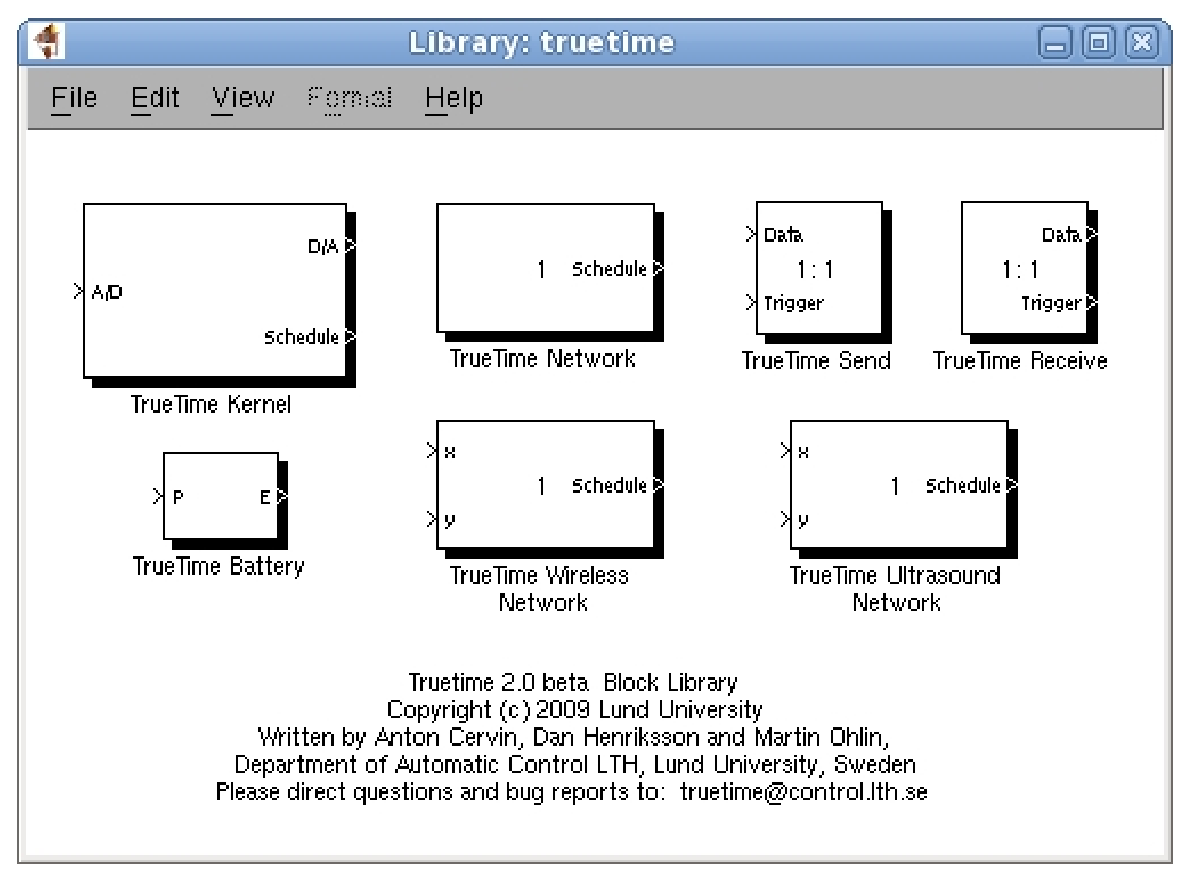
\includegraphics[scale=.5]{lib2.0beta.eps}
  \end{center}
  \caption{The \textsc{TrueTime} 2.0 block library.}
  \label{fig:library}
\end{figure}

\subsection{Compilation}
\label{sec:start_compile}
Since the \textsc{TrueTime} archive contains pre-compiled files, no
compilation should be required to run \textsc{TrueTime} with the M-file API.

% After starting Matlab and before running \textsc{TrueTime} \textit{for
%   the first time}, you must compile the \textsc{TrueTime} blocks and
% the MEX-functions for the \textsc{TrueTime} commands (unless you have
% downloaded the archive with pre-compiled files). This is done by
% issuing the command
% \begin{small}
% \begin{verbatim}
%   >> make_truetime
% \end{verbatim}
% \end{small}
% from the Matlab prompt. This performs all necessary compilation needed
% to run the Matlab version of \textsc{TrueTime}. For instructions on
% how to compile individual simulations in the C++ case, see
% Section~\ref{sec:compile}. 

However, \textsc{TrueTime} also supports simulations written in C++
code, which then must be compiled. In this case, you first need to
configure your C++ compiler in Matlab. This can be done by issuing
the command

\begin{small}
\begin{verbatim}
  >> mex -setup C++
\end{verbatim}
\end{small}

In the setup, make sure that you change from the Matlab default
compiler to a proper C++ compiler. For more detailed instructions on how to
compile individual simulations, see Section~\ref{sec:compile} in this
manual.

\section{Using the Simulator}

The \textsc{TrueTime} blocks are connected with ordinary Simulink
blocks to form a real-time control system, see Figure~\ref{fig:ex}.
Before a simulation can be run, however, it is necessary to initialize
kernel blocks and network blocks, and to create tasks, interrupt
handlers, timers, events, monitors, etc for the simulation.

As mentioned above, the initialization code and the code that is
executed during simulation may be written either as Matlab M-files or
as C++ code (for increased simulation speed). How the code functions
are defined and what must be provided during initialization will be
described below. It will also be described how the code is compiled to
executable Matlab code.

\begin{figure}[htbp]
  \begin{center}
    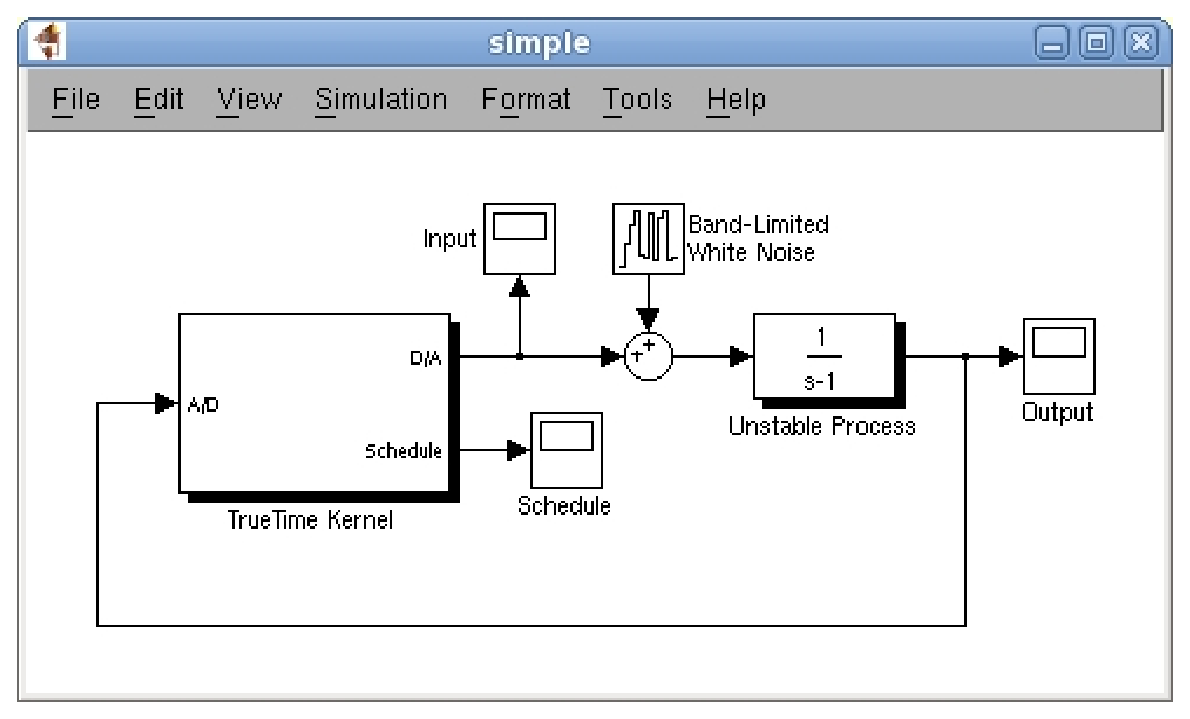
\includegraphics[scale=.5]{simple.eps}
  \end{center}
  \caption{A \textsc{TrueTime} Kernel block connected to a
    continuous plant.}
  \label{fig:ex}
\end{figure}

\section{Writing Code Functions}
The execution of tasks and interrupt handlers is defined by code
functions. A code function is further divided into code segments
according to the execution model shown in Figure~\ref{fig:timeline}.
All execution of user code is done in the beginning of each code
segment. The execution time of each segment should be returned by the
code function.

\begin{figure}[htbp]
  \begin{center}
    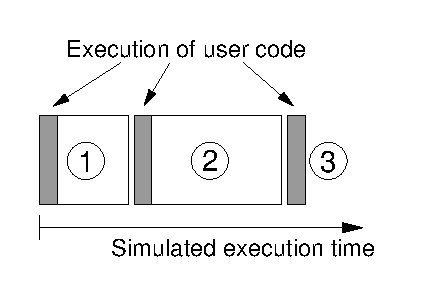
\includegraphics[scale=1.05]{timeline.eps}
  \end{center}
  \caption{The execution of user code is modeled by a sequence of
    segments executed in order by the kernel.}
  \label{fig:timeline}
\end{figure}

\subsection{Writing a Matlab Code Function}
\label{sec:mcode}
The syntax of a Matlab code function implementing a simple
P-controller is given by Listing~\ref{list:code1}.

The variable \texttt{segment} determines which segment that should be
executed, and \texttt{data} is a user-defined data structure that has
been associated with the task when it was created (see
\texttt{ttCreateTask} and \texttt{ttCreatePeriodicTask} in the command
reference). The data is updated and returned by the code function. The
code function also returns the execution time of the executed segment.

In this example, the execution time of the first segment is 2~ms. This
means that the delay from input to output for this task will be at
least 2~ms. However, preemption from higher priority tasks may cause
the delay to be longer. The second segment returns a negative
execution time. This is used to indicate end of execution, i.e. that
there are no more segments to execute.

\texttt{ttAnalogIn} and \texttt{ttAnalogOut} are real-time primitives
used to read and write signals to the environment. Detailed
descriptions of these functions can be found in the command reference
at the end of this manual.

\begin{listing}[b]\small
\caption{Example of a P-controller code function written in
  Matlab code.}
\label{list:code1}
\vspace{3mm}
\hrule
\begin{verbatim}
  function [exectime,data] = ctrl_code(segment, data)

  switch segment
    case 1
      y = ttAnalogIn(1);
      data.u = -data.K * y;
      exectime = data.exectime;
    case 2
      ttAnalogOut(1, data.u)
      exectime = -1;
  end
\end{verbatim}
\hrule
\end{listing}


\subsection{Writing a C++ Code Function}
Writing a code function in C++ follows a similar pattern as the code
function described in Listing~\ref{list:code1}. The corresponding C++
syntax for the P-controller code function is given in
Listing~\ref{list:code2}. We here assume the existence of a data
structure \texttt{Task\_Data} that contains the control signal $u$ and
the controller gain, $K$.

\subsection{Calling Simulink Block Diagrams}
In both the C++ and m-file cases, it is possible to call Simulink
block diagrams from within the code functions. This is a convenient
way to implement controllers. Listing~\ref{list:code3} shows an
example where the discrete PI-controller in Figure~\ref{fig:piblock}
is used in a code function. See the command reference at the end of
this manual for further explanation of the command
\texttt{ttCallBlockSystem}.

\begin{figure}[h]
  \centerline{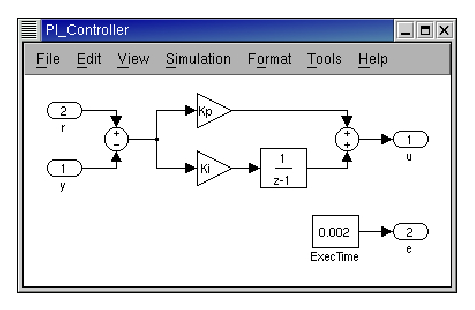
\includegraphics[scale=1.0]{block.ps}}
  \caption{Controllers represented using ordinary discrete
    Simulink blocks may be called from within the code functions. The
    only requirement is that the blocks are discrete with the sample
    time set to one.}
  \label{fig:piblock}
\end{figure}

\begin{listing}[b]\small
\caption{Simulink block diagrams are called from within code
  function using the function \texttt{ttCallBlockSystem}.}
\label{list:code3}
\vspace{3mm}
\hrule
\begin{verbatim}
     function [exectime, data] = PIcode(segment, data)

     switch segment,
       case 1,
         inp(1) = ttAnalogIn(1);
         inp(2) = ttAnalogIn(2);
         outp = ttCallBlockSystem(2, inp, 'PI_Controller');
         data.u = outp(1);
         exectime = outp(2);
       case 2,
         ttAnalogOut(1, data.u);
         exectime = -1; % finished
     end
\end{verbatim}
\hrule
\end{listing}
\clearpage

\section{Initialization}
\label{sec:initialization}
Initialization of a \textsc{TrueTime} kernel block involves specifying
the number of inputs and outputs of the block, defining the scheduling
policy, and creating tasks, interrupt handlers, events, monitors, etc
for the simulation. This is done in an initialization script for each
kernel block. The initialization script can (in the Matlab case) also
take an optional parameter to limit the number of similar code
functions. The other \textsc{TrueTime} kernel block parameters are
described in Section~\ref{sec:kernel}.

In the examples given below, the initialization script is called
\texttt{example\_init}, both in the Matlab and C++ cases. The optional
parameter is called {\tt argument} when it is used.

\subsection{Writing a Matlab Initialization Script}
\label{sec:minit}
The initialization code in Listing~\ref{list:init1} shows the minimum
of initialization needed for a \textsc{TrueTime} simulation. The
kernel is initialized by providing the number of inputs and outputs
and the scheduling policy using the function \texttt{ttInitKernel}. A
periodic task is created by the function
\texttt{ttCreatePeriodicTask}. The period of the task is given by the
init argument of the \textsc{TrueTime} Kernel block dialogue. (Note that the init argument may
be an arbitrary Matlab struct.) This task uses the code function
\texttt{Pcontroller} that was defined in Listing~\ref{list:code1}. See
the command reference for further explanation of the functions.

\begin{listing}[b]\small
\caption{Example of a \textsc{TrueTime} initialization script in the
  Matlab version. The kernel is initialized using the function
  \texttt{ttInitKernel}, and a periodic task is created that uses the
  P-controller code function from Listing~\ref{list:code1}. The period
of the controller is passed to the initialization script as a parameter.}
\label{list:init1}
\vspace{3mm}
\hrule
\begin{verbatim}
  function simple_init

  ttInitKernel('prioFP')

  data.K = 2;            % controller proportional gain
  data.exectime = 0.1;   % control task execution time
  starttime = 0.0;       % control task start time
  period = 0.5;          % control task period

  ttCreatePeriodicTask('ctrl_task', starttime, period, 'ctrl_code', data)
\end{verbatim}
\hrule
\end{listing}

In the Matlab case, you may experience that nothing changes in the
simulations, although changes are being made to the code functions or
the initialization script. If that is the case, type the following at
the Matlab prompt

\begin{small}
\begin{verbatim}
  >> clear functions
\end{verbatim}
\end{small}

To force Matlab to reload all functions at the start of each
simulation, issue the command (assuming that the model is named
\texttt{mymodel})

\begin{small}
\begin{verbatim}
  >> set_param('mymodel', 'InitFcn', 'clear functions')
\end{verbatim}
\end{small}

\begin{listing}[t]\small
\caption{Template for writing initialization scripts in C++. The final
  script is actually a complete Simulink S-function, since the included
  file, \texttt{ttkernel.cpp}, contains the Simulink callback functions
  that implement the kernel.}
\label{list:template}
\vspace{3mm}
\hrule
\begin{verbatim}
  #define S_FUNCTION_NAME filename
  #include "ttkernel.cpp"

  // insert your code functions here

  void init() {
  // perform the initialization
  }

  void cleanup() {
  // free dynamic memory allocated in this script
  }
\end{verbatim}
\hrule
\end{listing}


\subsection{Writing a C++ Initialization Script}
An initialization script in C++ must follow a certain format given by
the template in Listing~\ref{list:template}. The included file
\texttt{ttkernel.cpp} contains the Simulink callback functions that
implement the \textsc{TrueTime} kernel, meaning that the
initialization script is actually a complete Matlab S-function.
\texttt{filename} should be the name of the source file, e.g. if the
source file is called \texttt{example\_init.cpp},
\texttt{S\_FUNCTION\_NAME} should be defined to
\texttt{example\_init}.

The \texttt{init()}-function is called at the start of simulation
(from the Simulink callback function \texttt{mdlInitializeSizes}), and
it is here all initialization should be performed. The initial
argument supplied in the \textsc{TrueTime} Kernel block dialogue can
be retrieved using the function \texttt{ttGetInitArg}. Any dynamic
memory allocated from the \texttt{init()}-function can be deallocated
from the \texttt{cleanup()}-function, which is called at the end of
simulation. A pointer to aritrary user data can be stored using
\texttt{ttSetUserData} and later retrieved using
\texttt{ttGetUserData}.

The C++ version of the Matlab initialization
script of Listing~\ref{list:init1} is given in
Listing~\ref{list:init2}.

\begin{listing}[p]\small
\caption{Example of a \textsc{TrueTime} initialization script in the
  C++ version. Corresponds to the Matlab version from Listing~\ref{list:init1}.}
\label{list:init2}
\vspace{3mm}
\hrule
\begin{verbatim}
  #define S_FUNCTION_NAME simple_init
  #include "ttkernel.cpp"

  // Data structure used for the task data
  class CtrlData {
  public:
    double u;  
    double K;
    double exectime;
  };

  // Code function for the P-controller
  double ctrl_code(int segment, void* data) {

    CtrlData *d = (CtrlData*)data;
    double y;
  
    switch (segment) {
    case 1:
      y = ttAnalogIn(1);
      d->u = - d->K * y;
      return d->exectime;
    case 2:
      ttAnalogOut(1, d->u);
      return FINISHED;
    }
  }

  // Kernel init function    
  void init() {

    // Allocate memory for the task
    CtrlData *data = new CtrlData;
  
    // Store a pointer to the task data so that it can be cleaned up
    ttSetUserData(data);

    data->K = 2.0;
    data->exectime = 0.1;

    ttInitKernel(prioFP);
    ttCreatePeriodicTask("ctrl_task", 0.0, 0.5, ctrl_code, data);
  }

  // Kernel cleanup function
  void cleanup() {

    delete (CtrlData *)ttGetUserData();
  }
\end{verbatim}
\hrule
\end{listing}

\section{Compilation}
\label{sec:compile}

Compilation requires that a proper C++ compiler has been configured in
Matlab as described in Section~\ref{sec:start_compile}. If needed, the
\textsc{TrueTime} kernel may be re-compiled by issuing the command

\begin{small}
\begin{verbatim}
  >> make_truetime
\end{verbatim}
\end{small}

from the Matlab prompt. This script compiles the kernel and network
S-functions and the MEX-files for the \textsc{TrueTime} primitives.

In the C++ case, the initialization script (\texttt{example\_init.cpp}
in the example from the previous section) must be compiled to produce
a Matlab MEX-file for the simulation. This is done by the command

\begin{small}
\begin{verbatim}
  >> ttmex example_init.cpp
\end{verbatim}
\end{small}

The initialization file needs to be recompiled each time changes are made to
the code functions or to the initialization functions.

{\em Note:} The \texttt{ttmex} command is the same as the ordinary
\texttt{mex} command but includes the path to the kernel files
(\texttt{ttkernel.cpp}) automatically.


\section{The \textsc{TrueTime} Kernel}
\label{sec:kernel}

The kernel block is configured through the block mask dialog, see
Figure~\ref{fig:kdialog}, with the following parameters (some
parameters can also be set at run-time with the command {\tt
  ttSetKernelParameter}):

\begin{description}
\item[Init function] The name of the initialization script,
  see Section~\ref{sec:initialization}.
\item[Init function argument] an optional argument to the
  initialization script. This can be any Matlab struct.
\item[Battery] Enable this check box if the kernel should depend on a power source.
\item[Clock drift] The time drift, $0.01$ if the local time should run
  $1\%$ faster than the nominal time (the actual simulation time).
\item[Clock offset] A constant time offset from the nominal time.
\end{description}

\begin{figure}[tbp]
  \centerline{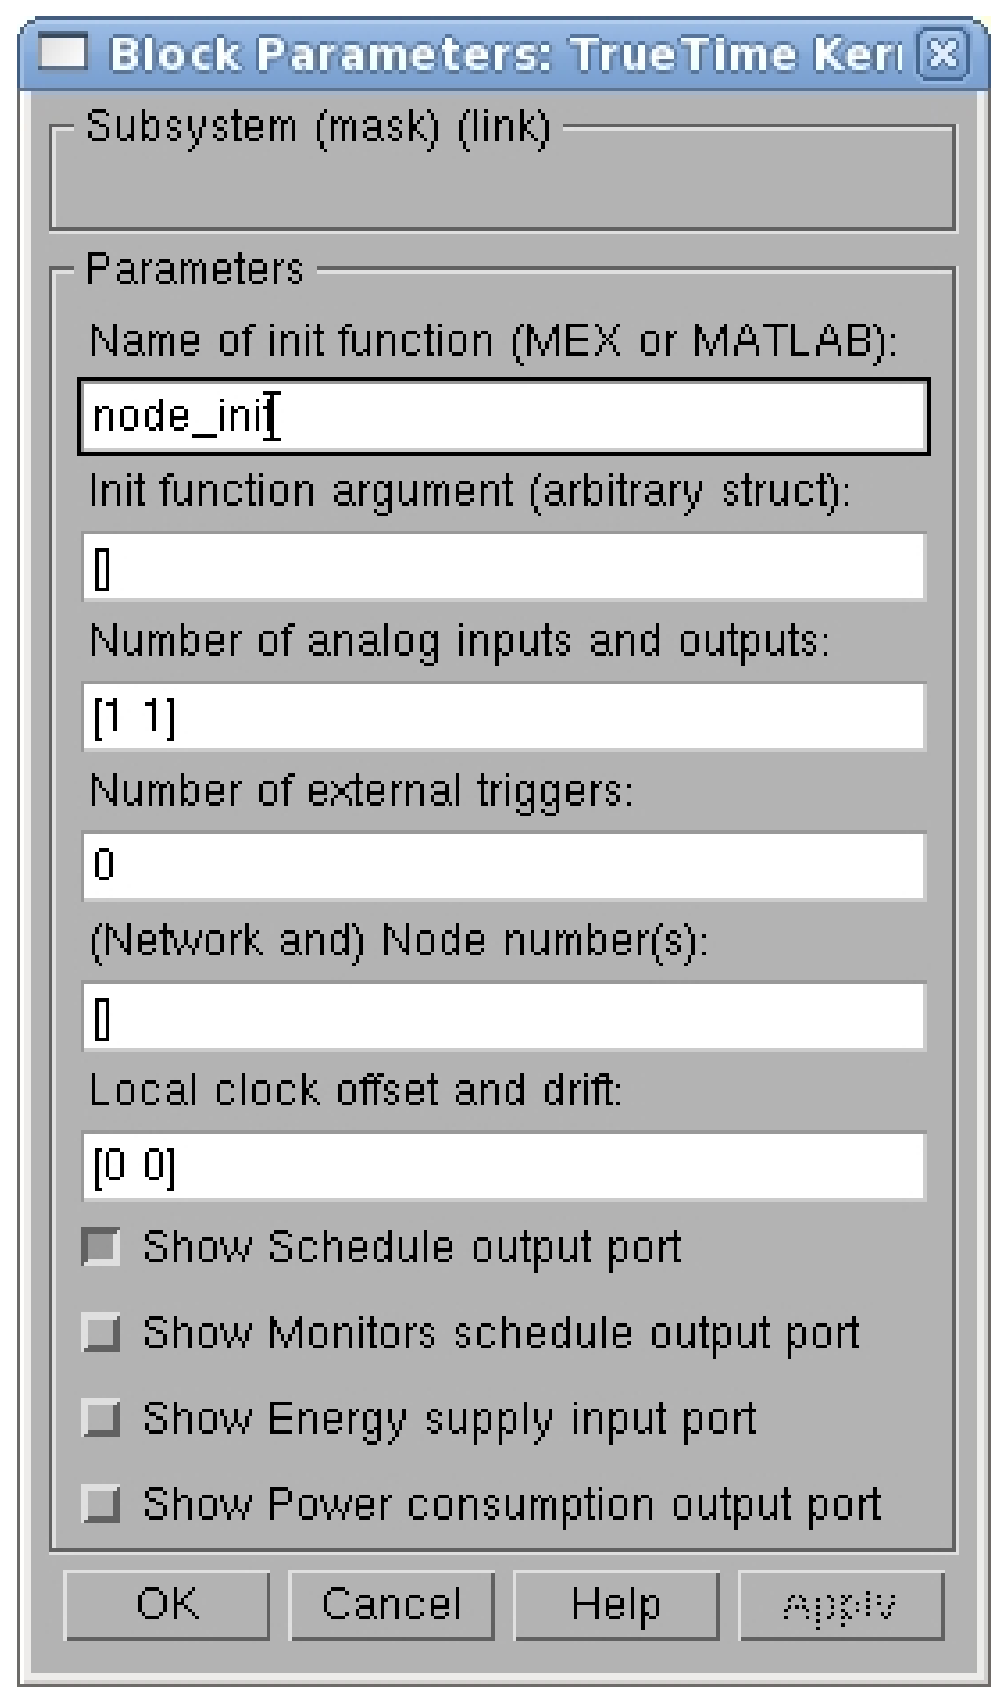
\includegraphics[scale=0.3]{kdialog.eps}}
  \caption{The dialog of the \textsc{TrueTime} kernel block.}
  \label{fig:kdialog}
\end{figure}

\subsection{Dynamic Voltage Scaling}
With the use of {\tt ttSetKernelParameter}, the current execution speed of the
kernel can be set and also the current power consumption. This makes it
possible to simulate Dynamic Voltage Scaling. This functionality can
be useful together with the battery block, see Section~\ref{sec:battery}.

\section{The \textsc{TrueTime} Network}

The \textsc{TrueTime} network block simulates medium access and packet
transmission in a local area network. When a node tries to transmit a
message (using the primitive \texttt{ttSendMsg}), a triggering signal
is sent to the network block on the corresponding input channel. When
the simulated transmission of the message is finished, the network
block sends a new triggering signal on the output channel
corresponding to the receiving node. The transmitted message is put in
a buffer at the receiving computer node. A message contains
information about the sending and the receiving computer node,
arbitrary user data (typically measurement signals or control
signals), the length of the message, and optional real-time attributes
such as a priority or a deadline.

Six simple models of networks are supported: CSMA/CD (e.g. Ethernet),
CSMA/ AMP (e.g. CAN), Round Robin (e.g. Token Bus), FDMA, TDMA (e.g.
TTP), and Switched Ethernet. The propagation delay is ignored, since
it is typically very small in a local area network. Only packet-level
simulation is supported---it is assumed that higher protocol levels in
the kernel nodes have divided long messages into packets, etc.

\begin{figure}[tbp]
  \centerline{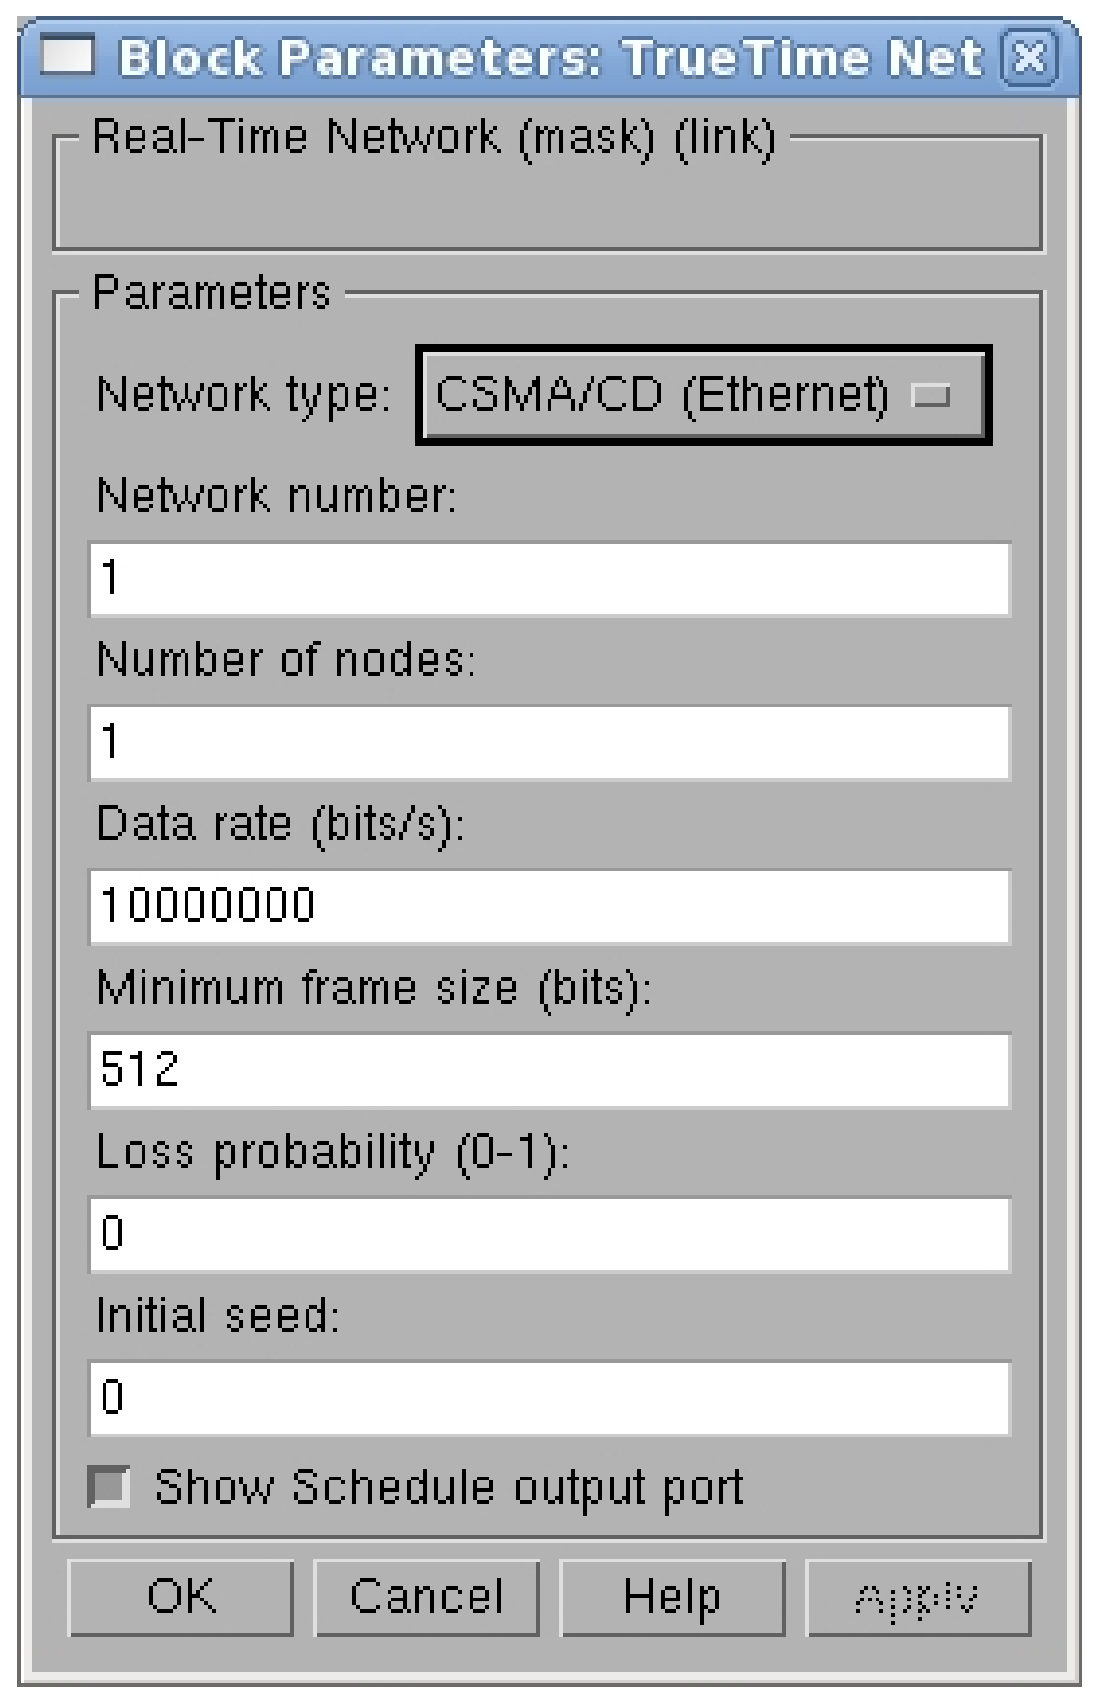
\includegraphics[scale=0.3]{nwdialog.eps}}
  \caption{The dialog of the \textsc{TrueTime} network block.}
  \label{fig:nwdialog}
\end{figure}

The network block is configured through the block mask dialog, see
Figure~\ref{fig:nwdialog}. Using the command {\tt
  ttSetNetworkParameter}, see Section~\ref{sec:command_reference}, it
is also possible to change some parameters on a per node basis. The
following network parameters are common to all models:

\begin{description}
\item[Network number] The number of the network block. The networks
  must be numbered from 1 and upwards. Wired and wireless networks are
  not allowed to use the same number.
\item[Number of nodes] The number of nodes that are connected to the
  network. This number will determine the size of the {\tt Snd}, {\tt
    Rcv} and {\tt Schedule} input and outputs of the block.
\item[Data rate (bits/s)] The speed of the network.
\item[Minimum frame size (bits)] A message or frame shorter than this
  will be padded to give the minimum length. Denotes the minimum frame
  size, including any overhead introduced by the protocol. E.g., the
  minimum Ethernet frame size, including a 14-byte header and a 4-byte
  CRC, is 512 bits.
%\item[Pre-processing delay (s)] The time a message is
%delayed by the network interface on the sending end. This can be used
%to model, e.g., a slow serial connection between the computer and the
%network interface.
%\item[Post-processing delay (s)] The time a message is
%delayed by the network interface on the receiving end.
\item[Loss probability (0--1)] The probability that a network message
  is lost during transmission. Lost messages will consume network
  bandwidth, but will never arrive at the destination.
\end{description}

\subsection{CSMA/CD (Ethernet)}
CSMA/CD stands for Carrier Sense Multiple Access with Collision
Detection. If the network is busy, the sender will wait until it
occurs to be free. A collision will occur if a message
is transmitted  within 1 microsecond of another (this corresponds to
the propagation delay in a 200 m cable; the actual number is not very
important since collisions are only likely to occur when two or more
nodes are waiting for the cable to be idle). When a collision occurs,
the sender will back off for a time defined by
\[
t_\mathit{backoff} = \text{minimum frame size} \ /\  \text{data rate} \times R
\]
where $R = \mathrm{rand}(0,\,2^K-1)$ (discrete uniform distribution) and
$K$ is the number of collisions in a row (but maximum 10---there is no
upper limit on the number of retransmissions, however). Note that for
CSMA/CD, minimum frame size cannot be 0.

After waiting, the node will attempt to retransmit. In an example
where two nodes are  waiting for a third node to finish its
transmission, they will first collide with probability 1, then with
probability 1/2 ($K=1$), then 1/4 
($K=2$), and so on.

\subsection{CSMA/AMP (CAN)}
CSMA/AMP stands for Carrier Sense Multiple Access with Arbitration on
Message Priority. If the network is busy, the sender will wait until it
occurs to be free. If a collision occurs (again, if two transmissions
are being started within 1 microsecond), the message with the highest
priority (the lowest priority number) will continue to 
be transmitted. If two messages with the same priority seek
transmission simultaneously, an arbitrary choice is made as to which
is transmitted first. (In real CAN applications, all sending nodes
have a unique identifier, which serves as the message priority.)

\subsection{Round Robin (Token Bus)}
The nodes in the network take turns (from lowest to highest node
number) to transmit one frame each. Between turns, the network is idle
for a time
\[
t_\mathit{idle} = \text{minimum frame size} \  /\  \text{date rate},
\]
representing the time to pass a token to the next node.

\subsection{FDMA}
FDMA stands for Frequency Division Multiple Access. The transmissions
of the different nodes are completely independent and no collisions
can occur. In this mode, there is an extra attribute

\begin{description}
\item[Bandwidth allocations] A vector of shares for the sender nodes
  which must sum to at most one.
\end{description}

The actual bit rate of a sender is computed as (allocated bandwidth
$\times$ data rate).

\subsection{TDMA (TTP)}
TDMA stands for Time Division Multiple Access. Works similar to FDMA,
except that each node has 100 \% of the bandwidth but only 
in its scheduled slots. If a full frame cannot be transmitted in
a slot, the transmission will continue in the next scheduled slot,
without any extra penalty. Note that overhead is added to each frame
just as in the other protocols. The extra attributes are

\begin{description}
\item[Slot size (bits)] The size of a sending slot. The slot time is
  hence given by 
\[
t_\mathit{slot} = \text{slot size} \ / \ \text{data rate}.
\]
\item[Schedule] A vector of sender node ID's (1 \ldots nbrOfNodes) specifying a
cyclic send schedule. A zero is also an allowed node ID, meaning that
no-one is allowed to transmit in that time slot.
\end{description}

\subsection{Switched Ethernet}
In Switched Ethernet, each node in the network has its own,
full-duplex connection to a central switch. Compared to an ordinary
Ethernet, there will never be any collisions on the network segments
in a Switched Ethernet. The switch stores the received messages in a
buffer and then forwards them to the correct destination nodes. This
common scheme is known as {\em store and forward}.

If many messages in the switch are destined for the same node, they
are transmitted in FIFO order. There can be either one queue that
holds all the messages in the switch, or one queue for each output
segment. In case of heavy traffic and long message queues, the switch
may run out of memory. The following options are associated with the
Switched Ethernet:
\begin{description}
\item[Total switch memory (bits)] This is the total amount of memory
  available for storing messages in the switch. An amount of memory
  equal to the length of the message is allocated when the message has
  been fully received in the switch. The same memory is deallocated
  when the complete message has reached its final destination node.
\item[Switch buffer type] This setting describes how the memory is
  allocated in the switch. {\em Common buffer} means that all messages
  are stored in a single FIFO queue and share the same memory area.
  {\em Symmetric output buffers} means that the memory is divided into
  $n$ equal parts, one for each output segment connected to the
  switch. When one output queue runs out of memory, no more messages
  can be stored in that particular queue.
\item[Switch overflow behavior] This option describes what happens
  when the \linebreak switch has run out of memory. When the complete
  message has been received in the switch, it is deleted. {\em
    Retransmit} means that the switch then informs the sending node
  that it should try to retransmit the message. {\em Drop} means that
  no notification is given---the message is simply deleted.
\end{description}

\subsection{FlexRay}
In FlexRay the transmission cycle consists of three consecutive segments.
The first, \emph{static}, segment works similar to the TDMA protocol. The
nodes take turns to transmit data according to a schedule. A node can
only transmit when it is scheduled to do so. If the node has nothing
to transmit, the network is idle until it is time to change node
according to the schedule.  

The second, \emph{dynamic}, segment is divided into a number of small
mini-slots with a corresponding schedule. In each mini-slot the
scheduled node may start to transmit but only if the transmission is finished
before the end of the dynamic segment. The transmission can, unlike
in the static segment, continue to transmit when the mini-slot is
over. If the scheduled node was nothing to transmit, the network will
be idle the time it takes to transmit a frame the size of a mini-slot.
Note that a message can be too large to ever be transmitted and thus
blocks the sending node for transmitting messages in the dynamic segment. 

The third, \emph{idle}, segment where the network can't transmit anything.
This segment is used to simulate both the symbol window and the
network idle time in FlexRay.  

The FlexRay protocol has the following extra parameters:
\begin{description}
\item[Slotsize (bits)] Size of a slot for the static segment.
\item[Static schedule] Transmission schedule for the static segment.
\item[Dynamic schedule] Transmission schedule for the dynamic segment.
\item[Mini slot size (bits)] Size of a mini-slot for the dynamic
  segment. 
\item[Network idle time (bits)] Size of the idle segment
\end{description}
The static segment is length(Static schedule)*Slotsize/dataRate seconds
long and the dynamic segment will similarly be
length(Dynamic schedule)*Minislotsize/dataRate seconds long. The network will
then be idle for networkIdle/dataRate seconds. Additionally, both
senders have an extra field where it is specified wheter the message
should be transmitted in the static or in the dynamic segment. 

\subsection{PROFINET IO}
The PROFINET IO send cycle consists of three intervals,
synchroniztion, RT Class 3 and RT Class 1/NRT. RT Class 2 is not
supported in this implementation. 

\begin{description}
\item[Synchronization] 
 During the synchronization interval no node can send or receive
 messages. The duration of the synchronization interval is
 $\frac{\text{\textbf{Synchronization
       length}}}{\text{\textbf{Datarate}}}$ seconds.

\item[RT Class 3 / IRT]
  Following the synchronization interval is the \emph{RT Class 3 / IRT
  (Isochronous Real Time)} interval. The transmissions during the are
  determined by the \textbf{IRT schedule}. The schedule is represented as a
  matrix with 5 columns and as many rows as messages to be sent during
  an IRT-interval. The first column specifies the ID of the message
  that should be transmitted. The message ID should be an integer
  larger than zero. The second and third column specifies from which
  node the message should be sent from and sent to respectively. The
  fourth column specifies the time, in seconds, when the message
  should be sent relative the start of the IRT interval. The fifth
  column specifies how long time it takes to propagate the message
  from sender to receiver.

  The latest incoming message in each node is saved and is retransmitted
  in each the IRT interval. 
  
  Broadcasting is not supported in the IRT interval.
\item[RT Class 1/NRT]
The third and final interval is the \emph{RT Class 1 / NRT (Non Real Time)}
interval. The length of the interval is determined by the user by
setting the \textbf{NRT length [bits]} parameter. In the field labeled Node
connection graph, the user has to specify how the different nodes are
connected. The \textbf{Node connection graph} should be represented as
a square matrix with the same number of rows and column as there are
nodes in the network. Each element $(x, y)$ in the matrix represents to
which node a message, currently in node $x$, should be transmitted to on
its way to node $y$. This way all messages will be transmitted in a
deterministic fashion even if there exists multiple possible paths
from the sending to the receiving node in the network.  

Each node is considered to have 4 ports and can thus be connected to 4
or less other nodes. An incoming message is considered to be a NRT
message if it's ID is equal to zero.

If a message is being transmitted to a node that has an empty switch
queue the message will cut-through this node. This means that only the
address bits will be read before the node with the empty switch start
to transmit the message. The address is considered being composed of
the first 114 bits. 
\end{description}

PROFINET IO offers the possibility to sort queues by priority instead
of FIFO. This protocol shares two parameter fields with Switched
Ethernet; Total switch memory and Switch overflow behavior.

\clearpage
\section{The \textsc{TrueTime} Wireless Network}

The usage of the wireless network block is similar to and works in the
same way as the wired one. To also take the path-loss of the radio
signals into account, it has {\tt x} and {\tt y} inputs to specify the
true location of the nodes. Two network protocols are supported at
this moment: IEEE 802.11b/g (WLAN) and IEEE 802.15.4 (ZigBee). Some
more technical details about the wireless network can be found
in~\cite{ohlin06lic}. The radio model used includes support for:
\begin{itemize}
\item Ad-hoc wireless networks.
\item Isotropic antenna.
\item Inability to send and receive messages at the same time.
\item Path loss of radio signals modeled as $\frac{1}{d^a}$ where $d$
  is the distance in meters and $a$ is a parameter chosen to
  model the environment.
\item Interference from other terminals.
\end{itemize}

\begin{figure}[tbp]
  \centerline{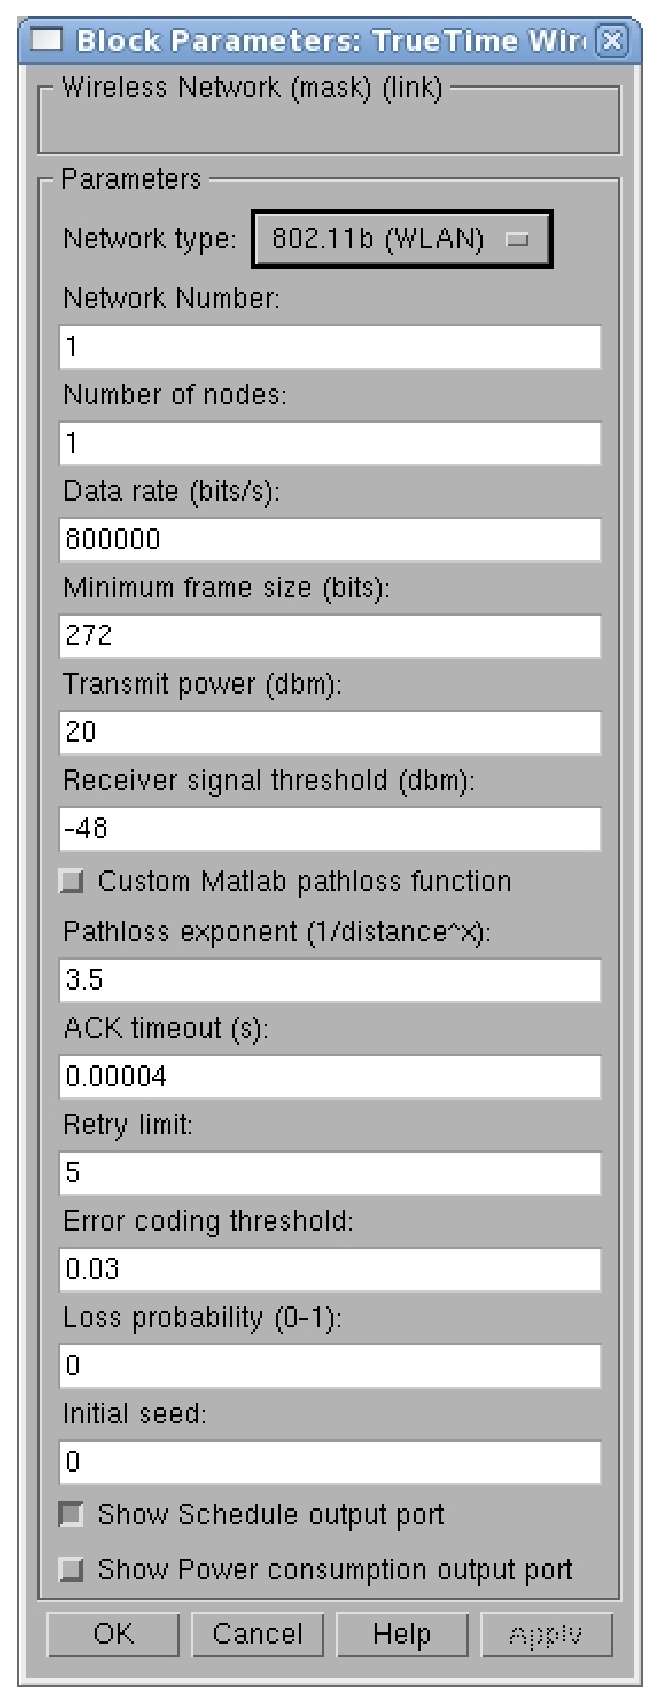
\includegraphics[scale=0.4]{wnwdialog}}
  \caption{The dialog of the \textsc{TrueTime} wireless network block.}
  \label{fig:wnwdialog}
\end{figure}

The wireless network block is configured through the block mask
dialog, see Figure~\ref{fig:wnwdialog}. Some parameters can also be
set on a per node basis with the command {\tt ttSetNetworkParameter}.
The following parameters are common to all models:

\begin{description}
\item[Network type] Determines the MAC protocol to be used. Can
  be either $802.11$b/g (WLAN) or $802.15.4$ (ZigBee).
\item[Network number] The number of the network block. The networks
  must be numbered from 1 and upwards. Wired and wireless networks are
  not allowed to use the same number.
\item[Number of nodes] The number of nodes that are connected to the
  network. This number will determine the size of the {\tt Snd}, {\tt
    Rcv} and {\tt Schedule} input and outputs of the block.
\item[Data rate (bits/s)] The speed of the network.
\item[Minimum frame size (bits)] A message or frame shorter than this
  will be padded to give the minimum length. Denotes the minimum frame
  size, including any overhead introduced by the protocol. E.g., most
  network protocols have a fixed number of header and tail bits, so
  the frame must be at least $sizeof(header)+sizeof(tail)$ long.
\item[Transmit power] Determines how strong the radio signal will be,
  and thereby how long it will reach.
\item[Receiver signal threshold] If the received energy is above this
  threshold, then the medium is accounted as busy.
\item[Path-loss exponent] The path loss of the radio signal is modeled
  as $\frac{1}{d^a}$ where $d$ is the distance in meters and $a$ is a
  suitably chosen parameter to model the environment. Typically chosen
  in the interval 2-4.
\item[ACK timeout] The time a sending node will wait for an ACK
  message before concluding that the message was lost and retransmit
  it.
\item[Retry limit] The maximum number of times a node will try to
  retransmit a message before giving up.
\item[Error coding threshold] A number in the interval $[0,1]$ which
  defines the percentage of block errors in a message that the coding
  can handle. For example, certain coding schemes can fully
  reconstruct a message if it has less than $3$\% block errors. The
  number of block errors are calculated using the signal-to-noise ratio,
  where the noise is all other ongoing transmissions.
\end{description}

\subsection{802.11b/g (WLAN)}
IEEE 802.11b/g is used in many laptops and mobile devices of today.
The protocol is based on CSMA/CA with some modifications. 

In the simulation, a package transmission is modeled like this: The node that wants to
transmit a packet checks to see if the medium is idle. The
transmission may proceed, if the medium is found to be idle, and has
stayed so for 50 $\mu$s. If, on the other hand, the medium is found to be busy, a random
back-off time is chosen and decremented in the same way as when
colliding (described later in this section). When a node starts to
transmit, its relative
position to all other nodes in the same network is calculated, and
the signal level in all those nodes are calculated according to the
path-loss formula $\frac{1}{d^a}$. 
%
%A package transmission is modeled like this: The node that wants to
%transmit a packet waits for the medium to be idle for a time specified
%in the standard (50 $\mu$s when using DSSS). After that, the package
%is sent on the network. When a node starts to transmit, its relative
%position to all other nodes in the same network are calculated, and
%the signal level in all those nodes are calculated according to the
%path-loss formula $\frac{1}{d^a}$. 

The signal is assumed to be possible to detect if the signal level in
the receiving node is larger than the {\bf receiver signal threshold}.
If this is the case, then the signal-to-noise ratio (SNR) is
calculated and used to find the block error rate (BLER). Note that all
other transmissions add to the background noise when calculating the
SNR. The BLER, together with the size of the message, is used to
calculate the number of bit errors in the message and if the
percentage of bit errors is lower than the {\bf error coding
  threshold}, then it is assumed that the channel coding scheme is
able to fully reconstruct the message. If there are (already) ongoing
transmissions from other nodes to the receiving node and their
respective SNRs are lower than the new one, then all those messages
are marked as collided. Also, if there are other ongoing transmissions
which the currently sending node reaches with its transmission, then
those messages may be marked as collided as well.

Note that a sending node does not know if its message is colliding,
therefore ACK messages are sent on the MAC protocol layer. From the
perspective of the sending node, lost messages and message collisions
are the same, i.e., no ACK is received. If no ACK is received during
{\bf ACK timeout}, the message is retransmitted after waiting
a random back-off time within a contention window. The contention
window size is doubled for every retransmission of a certain message.
The back-off timer is stopped if the medium is busy, or if it has not
been idle for at least 50 $\mu$s. There are only {\bf Retry limit} number of
retransmissions before the sender gives up on the message and it is
not retransmitted anymore.


\subsection{802.15.4 (ZigBee)}
ZigBee is a protocol designed with sensor and simple control networks in mind.
It has a rather low bandwidth, but also a really low power consumption.
Although it is based on CSMA/CA as 802.11b/g, it is much simpler and the
protocols are not the same.

The packet transmission model in ZigBee is similar to WLAN, but the
MAC procedure differ and is modeled as:

\begin{enumerate}
 \item Initialize:\\
   NB=$0$\\
   BE=macMinBE
% \item Delay for $random(2^{BE}-1)$ unit backoff periods
 \item Delay for a random number of backoff periods in the interval
   $[0, 2^{BE}-1]$
% \item Check if the medium is idle:\\
 \item Is the medium idle?\\
   \hspace*{5mm}  if yes: send\\
   \hspace*{5mm}  else: goto $4$
 \item Update the backoff counters:\\
   NB=NB$+1$\\
   BE=min(BE$+1$, aMaxBE)
% \item Check if $NB>macMaxCSMABackoffs$:\\
 \item Is NB>macMaxCSMABackoffs?\\
   \hspace*{5mm}  if yes: drop the packet\\
   \hspace*{5mm}  else: goto $2$
\end{enumerate}
The variable names are taken from the standard to make comparisons
easier. A small explanation of their names is provided below.
\begin{description}
\item[NB] Number of backoffs.
\item[BE] Backoff exponent.
\item[macMinBE] The minimum value of the backoff exponent in the
  CSMA/CA algorithm. The default value is $3$.
\item[aMaxBE] The maximum value of the backoff exponent in the CSMA/CA
  algorithm. The default value is $5$.
\item[macMaxCSMABackoffs] The maximum number of backoffs the CSMA/CA
algorithm will attempt before declaring a channel access failure. The
default value is $4$.
\end{description}

\subsection{Calculation of Error Probabilities}
During the calculation of error probabilities, it is for simplicity
assumed that
 BPSK\footnote{Binary Phase Shift Keying (BPSK) is a means of transmitting
   symbols by altering the phase of a reference signal. It uses two
   phases separated by $180^\circ$ and is hence binary.} is always used in the transmissions.
This is of course an approximation, but it relates well to reality.

Assume that a symbol is sent, in our case this is a bit, i.e., a $0$
or a $1$. Additive white Gaussian noise gives a probability density
function for the received symbol, that for some signal-to-noise ratio
may look like Figure~\ref{fig:error}. A threshold is then used to
decide if the received symbol is a $0$ or a $1$. The decision
threshold is marked as a line in the middle of the figure. The darker
area to the left of the threshold gives the probability of a symbol
error. A higher signal to noise ratio translates the curve to the
right, making
% this area and therefore also 
the probability of error smaller.

The above standard procedure should ideally be performed for every bit
in the message. The total number of calculated bit errors should then
be compared to the error coding threshold. This is, however, not done,
because it would be very computationally expensive. Instead, the
maximum noise level during the transmission is saved, and used to
calculate the worst case SNR. By assuming that bit errors in a message
are uncorrelated, it is deduced that the number of bit errors, $X$,
belongs to a binomial distribution $X\in Bin(n,p)$, where $n$ is the
number of bits in the message, and $p$ is the probability that a
certain bit is erroneous. If the value of $n$ is large, the binomial
distribution can be approximated with a normal distribution, using the
central limit theorem. This gives that $X\in N(np,\sqrt{npq})$ where
$q=1-p$. What we are really interested in is the probability that
$bn$, where $b$ is the error coding threshold, is larger than the
total number of bit errors in a message. This probability is
calculated using
\[
P(X\le bn)=
\left\{
\begin{aligned}
\Phi(\frac{bn-np}{\sqrt{npq}}) && \mathrm{if} && bn-np> 0\\
1-\Phi(\frac{\left|bn-np\right|}{\sqrt{npq}}) && \mathrm{if} && bn-np\le 0
\end{aligned}
\right.
\]
where $\Phi$ is the standard normal cumulative distribution function.
%P(X\le bn)=\Phi(\frac{bn-np}{\sqrt{npq}})

\begin{figure}
  \centerline{
%
%\resizebox{0.8\textwidth}{!}{\includegraphics{error_no_ticks.eps}}
    \resizebox{0.6\textwidth}{!}{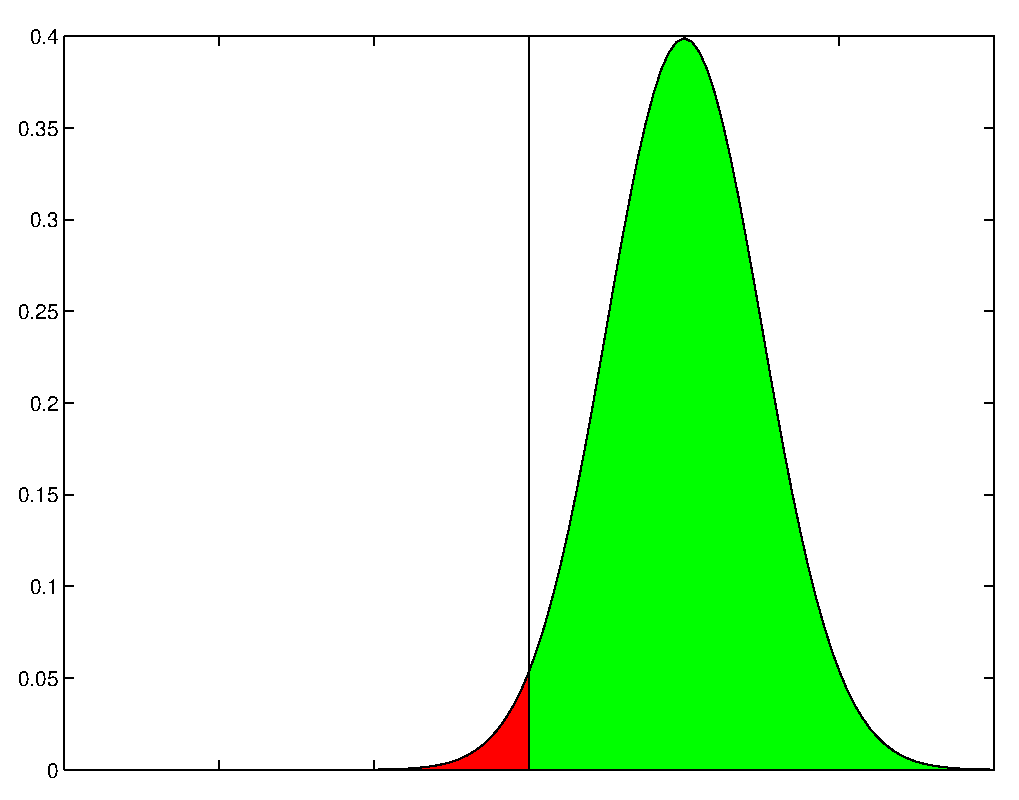
\includegraphics{error.eps}}
  }
  \caption{Probability density function for a received symbol when using
    % BPSK
    binary phase shift keying and additive white Gaussian noise. The
    line in the middle is the decision threshold. The area to the left
    of the threshold gives the probability of an erroneous decision.
    The area to the right gives the probability of a correct decision.}
  \label{fig:error}
\end{figure}

\subsubsection*{Example}

Assume that a message consists of $100$ bits, i.e., $n=100$. The
probability that a certain bit is erroneous has been calculated to
$0.1$ using the above method, i.e., $p=0.1$ and $q=1-p=0.9$. The error
coding threshold has been set to $5$\%, i.e., $b=0.05$. Then the
probability that we can decode the complete message is
\[
P(X\le
bn)=1-\Phi(\frac{\left|bn-np\right|}{\sqrt{npq}})=1-\Phi(\frac{5}{\sqrt{9}})\approx
0.0478
\]

\subsection{User-Defined Path-Loss Function}

The default path-loss function (or propagation model) used in the
TrueTime wireless simulations is
\[
P_{receiver}=\frac{1}{d^a}P_{sender}
\]
where $P$ is the power, $d$ is the distance in meters, and $a$ is a
parameter that can be chosen to model different environments. This
model is often used in simulations, but in some cases it can be
advantageous to use other models. TrueTime has the possibility to
register a user-defined path-loss function. The function is written as
a Matlab function (M-file or MEX-function) and can therefore take
advantage of all the built-in functions available in Matlab. In
particular, this includes the possibility to use persistent variables,
i.e., variables which are retained in memory between calls to the
function. The function can, for example, be used to model a
Rayleigh\footnote{In a Rayleigh fading, the relative speed of two
  nodes and the number of multiple paths that the signal takes from
  the sender to the receiver is taken into account. See
  Figure~\ref{fig:rayleigh} for an example.} fading or the blocking of
radio signals to and from certain points in the environment. At the
moment, nodes in the TrueTime framework only have $x$ and $y$
coordinates, but if a direction was to be introduced this function
could also be used to model directive effects in the antenna
behaviour.

\begin{figure}
  \centerline{
    \resizebox{0.8\textwidth}{!}{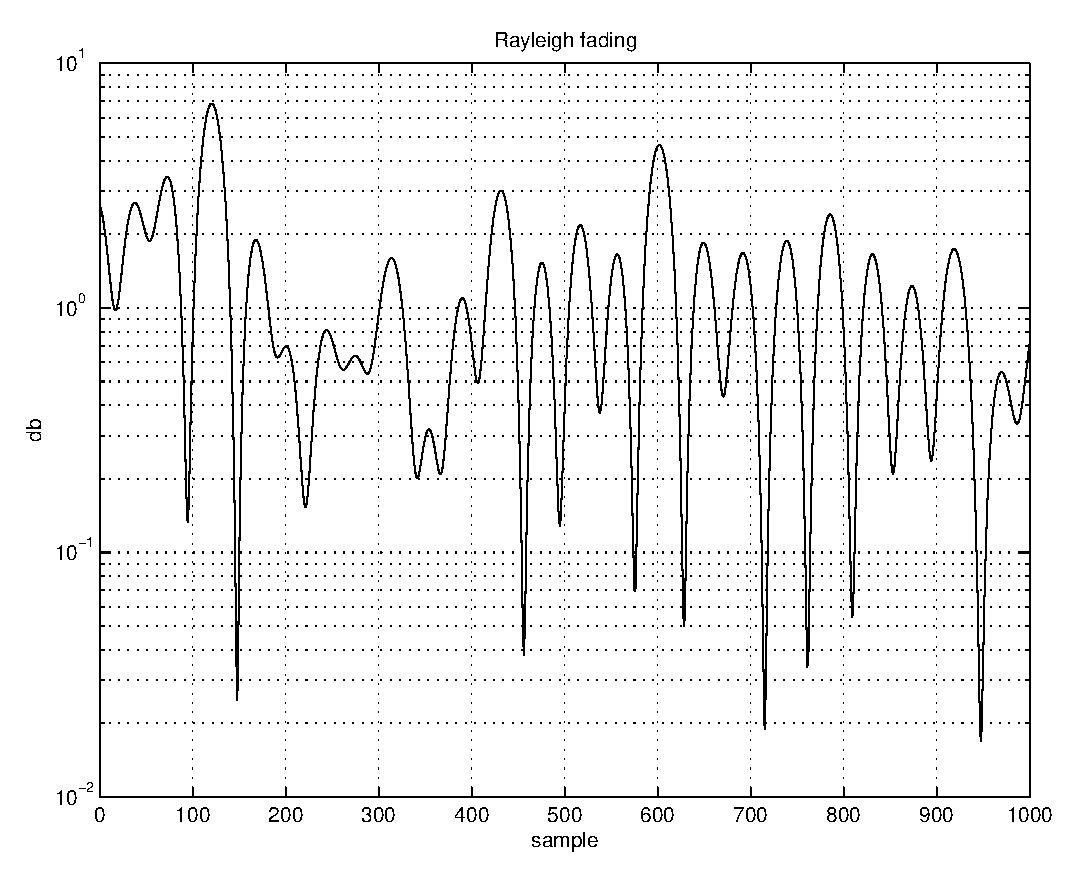
\includegraphics{rayleigh.eps}}
  }
  \caption{Example of a Rayleigh fading using a radio frequency of 2.4 MHz.
    Nodes moving with a relative speed of 6 km/h, 1 second sampling
    interval and 10 random phasers.}
  \label{fig:rayleigh}
\end{figure}

The Matlab function takes the following arguments
\begin{itemize}
\item Transmission power
\item Name of the sending node
\item $x$ and $y$ coordinates of the sending node
\item Name of the receiving node
\item $x$ and $y$ coordinates of the receiving node
\item Current simulation time
\end{itemize}
and returns the signal power in the receiving node. 
%A small example
%implementing the default path-loss function with a path-loss exponent of
%$3.5$ can be seen in Listing~\ref{listing:simple_example}.

A small example showing the structure of how a Rayleigh fading could
be implemented can be seen in Listing~\ref{listing:example}.

% \begin{listing}[htbp]\footnotesize %\small
% \caption{}
% \label{listing:simple_example}
% \vspace{3mm}
% \hrule
% \begin{verbatim}
% function [power]=simple(transmitPower, node1, x1, y1, node2, x2, y2, time)

% distance = sqrt((x1 - x2)^2 + (y1 - y2)^2);

% power = transmitPower/(distance+1)^3.5;
% \end{verbatim}
% \hrule
% \end{listing}

\begin{listing}[b]\footnotesize %\small
  \caption{Example of path-loss function modeling Rayleigh fading.}
  \label{listing:example}
  \vspace{3mm}
  \hrule
\begin{verbatim}
     function power = rayleigh(transmitPower, node1, x1, y1, node2, x2, y2, time)

     % Calculate the exponential pathloss
     distance = sqrt((x1 - x2)^2 + (y1 - y2)^2);
     power = transmitPower/(distance+1)^3.5;

     % Kalman filter to get the relative velocity of the two nodes
     velocity = kalman_velocity(node1, x1, y1, node2, x2, y2, time);
     % Calculate the rayleigh fading 
     factor = calculate_rayleigh(node1, node2, velocity, time);

     % Add the rayleigh fading to the exponential path loss
     power = power * factor;

\end{verbatim}
  \hrule
\end{listing}

To increase simulation speed, it is recommended to implement the
Matlab function as a C MEX-function.

\section{The \textsc{TrueTime} Battery}
\label{sec:battery}

The battery block has one parameter, the initial power, which can be
set using the configuration mask. To use the battery, enable the check
box in the kernel configuration mask and connect the output of the
battery to the {\tt E} input of the kernel block. Connect every power
drain such as the {\tt P} output of the kernel block, ordinary
Simulink models, and the wireless network block to the {\tt P} input
of the battery. The battery uses a simple integrator model, so it can
be both charged and recharged.

Note that the kernel will not execute any code if it is configured to
use batteries and the input {\tt P} to the kernel block is zero. See
the example in Section~\ref{sec:wireless} below for more details on
the use of \textsc{TrueTime} batteries.

\section{The \textsc{TrueTime} Standalone Network Blocks}
\label{sec:battery}
The standalone network blocks, named TrueTime Send and TrueTime Receive, as seen in Figure~\ref{fig:library}, can be used to send
messages using the network blocks without using kernel blocks. This
makes it possible to create TrueTime network simulations without
having to initialize kernels, create and install interrupt handlers,
etc. It is in other words possible to create a whole network
simulation in Simulink without any M-files at all. It is also possible
to mix these blocks with kernel blocks, so that some stations use the
standalone network blocks, while others use the standard {\tt ttSend}
and {\tt ttGetMsg} primitives from within a code function executing in
a kernel block.
\begin{figure}
  \centerline{
%    a)
    \resizebox{0.4\textwidth}{!}{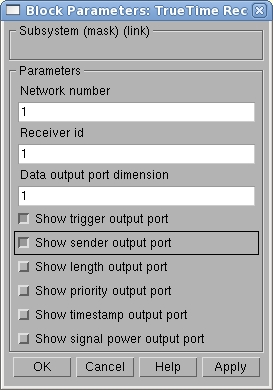
\includegraphics{ttgetmsgmask}}
%    b)
    \resizebox{0.4\textwidth}{!}{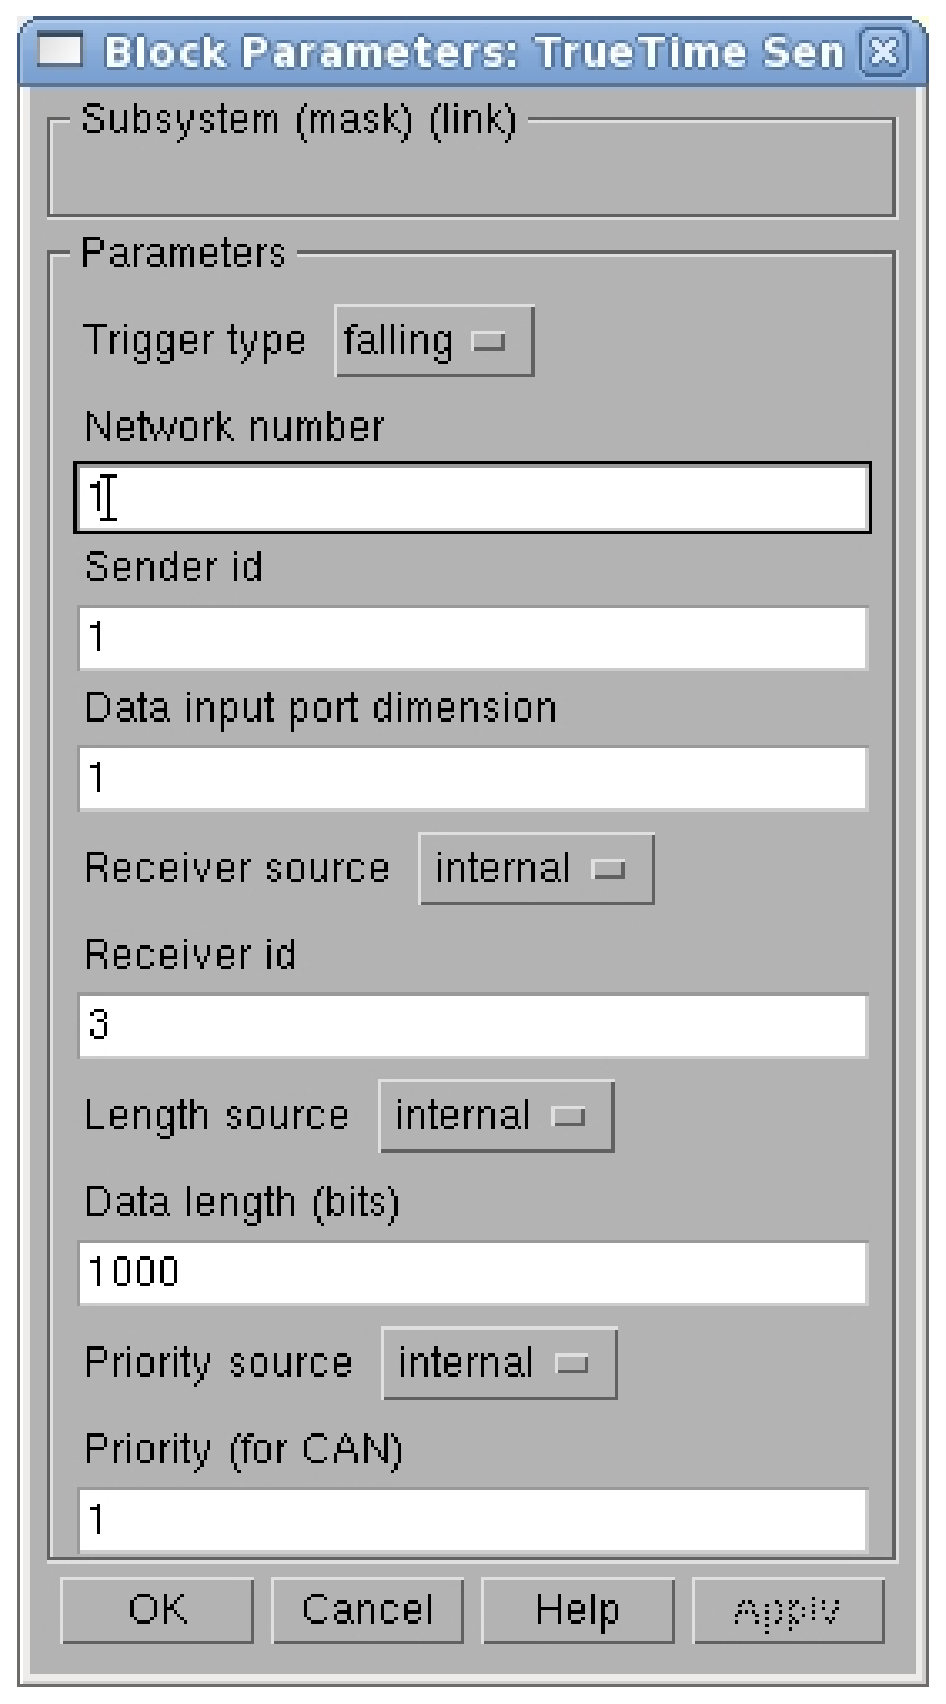
\includegraphics{ttsendmsgmask}}
  }
  \caption{The dialog of the TrueTime Send block to the left, and the
    dialog of the TrueTime Receive block to the right.}
  \label{fig:ttgetmsgmask}
\end{figure}

The standalone network blocks are configured through the block mask dialogs,
seen in Figure~\ref{fig:ttgetmsgmask}. The parameters are the same that are
used in the TrueTime Send and TrueTime Receive primitives.
The TrueTime Send block has a Simulink trigger input port, which can
be configured to trigger on raising, falling or either flanks. The
{\tt ttGetMsg} block has an optional trigger output port. The value of
the trigger output switches back and forth between 0 and 1 as messages are
received. This port can be used to trigger something that should be
executed after a new message has been received.


\section{Examples}
\label{sec:examples}

The directory \texttt{\$DIR/examples} contains ten examples:

\begin{longtable}{lp{0.75\hsize}}
{\tt simple} & Several different
ways of implementing a simple periodic controller are demonstrated.
Both M-file and C++ implementations are provided. \\
{\tt threeservos} & Illustrates task scheduling and control, where
three periodic control tasks execute on the same CPU. Both M-file and
C++ implementations are provided. \\
{\tt networked} & Demonstrates networked
control involving four computer nodes and the wired network block. Both M-file and
C++ implementations are provided, as well as an implementation using the
stand-alone network interface blocks. \\
%{\tt synch} &  Illustrates how to use monitors and events to simulate
%mutual exclusive access to shared variables. M-file
%implementation only. \\
%{\tt motes} & Demonstrates simulation and animation of collaborating mobile robots
%communicating over a wireless network. M-file implementation only. \\
{\tt wireless} & Demonstrates wireless networked control with
transmission power control to minimize the energy consumption. M-file implementation only.\\
{\tt AODV} & Illustrates how higher-layer communication protocols such as AODV routing
can be implemented in \textsc{TrueTime}.  M-file implementation only.\\
{\tt soccer} & A larger example showing simulation and animation of
ten mobile robots playing soccer. M-file implementation only.\\
{\tt RUNES\_demo} & A very large example with mobile robot navigation through a
sensor network using ultrasound trilateration. C++ implementation only.
\end{longtable}

The first three examples are provided in both Matlab and C++ versions.
However, the descriptions below will only treat the Matlab case. For
detailed instructions on how to compile the examples, see the
README-files in the corresponding example directories.

\subsection{PID-control of a DC-servo}
\label{sec:pid}

\subsubsection{Introduction}
The first example considers simple PID control of a DC-servo
process, and is intended to give a basic introduction to the
\textsc{TrueTime} simulation environment. The process is controlled by
a controller task implemented in a \textsc{TrueTime} kernel block.
Four different implementations of the controller task are provided to
show different ways to implement periodic activities. The files are
found in the directory \texttt{\$DIR/examples/simple/matlab}.

\subsubsection{Process and Controller}
The DC-servo is described by the continuous-time transfer function

\begin{equation}
\label{eq:servo}
G(s) = \frac{1000}{s(s+1)} 
\end{equation}

The PID-controller is implemented according to the following equations

\begin{equation}
  \begin{aligned}
    P(k) & =  K \cdot (\beta r(k) - y(k)) \\
    I(k+1) & = I(k) + \frac{Kh}{T_i}(r(k) - y(k)) \\
    D(k) & = a_d D(k-1) + b_d (y(k-1) - y(k)) \\
    u(k) & = P(k) + I(k) + D(k)
  \end{aligned}
  \label{eq:ctrl}
\end{equation}

where $a_d = \frac{T_d}{Nh+T_d}$ and $b_d = \frac{NKT_d}{Nh+T_d}$, see
\cite{ast+hagg95}. The controller parameters were chosen to give the
system a closed-loop bandwidth of $\omega_c = 20$ rad/s and a relative
damping of $\zeta = 0.7$.

\subsubsection{Simulation Files}

The initialization script (\texttt{servo\_init.m}) is given in an
abbreviated version in Listing~\ref{list:servoinit}. As seen in the
initialization script, it is possible to choose between four different
implementations of the periodic control task. They are specified by
the init function parameter in the kernel block dialog.

\begin{itemize}
\item \textit{Implementation 1}: Uses the \textsc{TrueTime}
  built-in support for periodic tasks, and the code function is given
  in the file \texttt{pidcode1.m}.
\item \textit{Implementation 2}: Also uses the \textsc{TrueTime}
  built-in support for periodic tasks, but the computation of the
  control signal in each sample is done by calling a Simulink block
  diagram. The code function is given in the file
  \texttt{pidcode2.m}. Since all the controller parameters and states
  are contained in the Simulink block, the task data (\texttt{data2})
  only consist of the control signal, $u$.
\item \textit{Implementation 3}: Implements the periodic task by
  using the \textsc{TrueTime} primitive \texttt{ttSleepUntil}. The
  code function is given in the file \texttt{pidcode3.m}.
\item \textit{Implementation 4}: Implements the periodic task by using
  a periodic timer. The associated interrupt handler samples the
  process and triggers task jobs. The handler and controller task
  communicate using a mailbox. The code functions for the handler and
  controller are given in the files \texttt{sampler} \texttt{code.m} and
  \texttt{pidcode4.m}, respectively.
\end{itemize}

\begin{listing}[b]\small
\caption{The initialization script for the PID-control example.}
\label{list:servoinit}
\vspace{3mm}
\hrule
\begin{verbatim}
  function servo_init(mode)

  ttInitKernel(2, 1, 'prioFP'); % nbrOfInputs, nbrOfOutputs, fixed priority

  period = 0.006;
  deadline = period;
  offset = 0.0; 
  prio = 1;

  data.K = 0.96;
  ... % more task data

switch mode,
 case 1, 
  % IMPLEMENTATION 1: using the built-in support for periodic tasks
  % 
  ttCreatePeriodicTask('pid_task',offset,period,prio,'pidcode1',data);

 case 2, 
  % IMPLEMENTATION 2: calling Simulink block within code function 
  %
  data2.u = 0; 
  ttCreatePeriodicTask('pid_task',offset,period,prio,'pidcode2',data2);

 case 3, 
  % IMPLEMENTATION 3: sleepUntil and loop back
  
  data.t = 0;
  ttCreateTask('pid_task',deadline,prio,'pidcode3',data);
  ttCreateJob('pid_task');

 case 4, 
  % IMPLEMENTATION 4: sampling in timer handler, triggers task job
  
  hdl_data.yChan = 2;
  ttCreateInterruptHandler('timer_handler',prio,'samplercode',hdl_data);
  ttCreatePeriodicTimer('timer',offset,period,'timer_handler');
  ttCreateMailbox('Samples',10);
  ttCreateTask('pid_task',deadline,prio,'pidcode4',data);
end
\end{verbatim}
\hrule
\end{listing}

\subsubsection{Simulations}

\begin{figure}[tbph]
  \begin{center}
    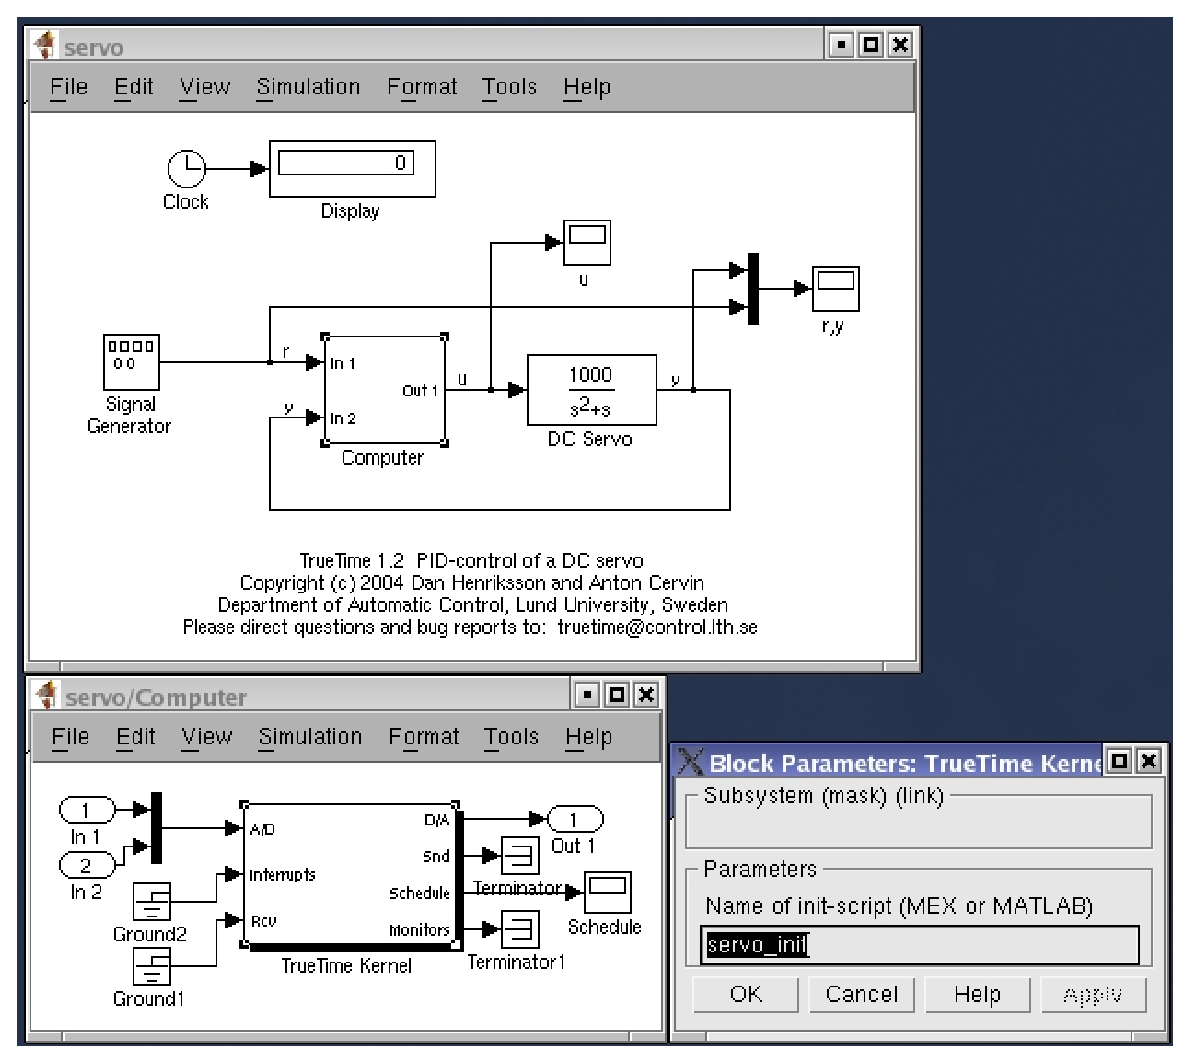
\includegraphics[scale=.65]{servo.ps}
  \end{center}
  \caption{The \textsc{TrueTime} model of the DC-servo system.}
  \label{fig:servo}
\end{figure}

The Simulink model is called \texttt{servo.mdl} and is given in
Figure~\ref{fig:servo}. Open the Simulink model and try the following

\begin{itemize}
\item Run a simulation and verify that the controller behaves as
  expected. Notice the computational delay of 2~ms in the control
  signal. Compare with the code function, \texttt{pidcode1.m}. Study
  the schedule plot (high=running, medium=ready, low=idle).
\item Try changing the execution time of the first segment of the code
  function, to simulate the effect of different input-output delays.
\item Change the sampling period and study the resulting control
  performance.
\item A PID-controller is implemented in the Simulink block
  \texttt{controller.mdl}. Change the init function parameter of the
  kernel block from $1$ to $2$, so that implementation 2 is used
  instead of $1$.
  Study the corresponding code function, \texttt{pidcode2.m}. This
  code function is using the Simulink block to compute the control
  signal in each sample.
\item Change to implementation 3 and run a simulation. Study the code
  function, \texttt{pidcode3.m}.
\item Change to implementation 4 and run a simulation. Study the code
  functions, \texttt{samplercode.m} and \texttt{pidcode4.m}. Notice
  the inclusion of the handler in the schedule plot.
\end{itemize} 

\subsection{Task Scheduling and Control}

\subsubsection{Introduction}
This example extends the simple PID control example from the previous
section to the case of three PID-tasks running concurrently on the
same CPU controlling three different DC-servo systems. The effect of
the scheduling policy on the global control performance is
demonstrated. The files are found in the directory
\texttt{\$DIR/examples/threeservos/matlab}.

\subsubsection{Simulations}
Open the Simulink model \texttt{threeservos.mdl} and try the following

\begin{itemize}
\item Make sure that rate-monotonic scheduling is specified by the
  function \linebreak \texttt{ttInitKernel} in the initialization script
  (\texttt{threeservos\_init.m}) and simulate the system. Study the
  computer schedule and the control performance. Task 1 will miss all
  its deadlines and the corresponding control loop is unstable.
\item Change the scheduling policy to earliest-deadline-first (change
  \texttt{'prioRM'} to \texttt{'prioEDF'}) and run a new simulation.
  Again study the computer schedule and the control performance. After
  an initial transient all tasks will miss their deadlines, but still the
  overall control performance is satisfactory.
\end{itemize} 

\subsection{Networked Control System}
\label{sec:dist}

\subsubsection{Introduction}
This example simulates networked control of the DC-servo
of Equation (\ref{eq:servo}). The example contains four computer
nodes, each represented by a \textsc{TrueTime} kernel block. A
time-driven sensor node samples the process periodically and sends the
samples over the network to the controller node. The control task in
this node calculates the control signal and sends the result to the
actuator node, where it is subsequently actuated. The simulation also
involves an interfering node sending disturbing traffic over the
network, and a disturbing high-priority task executing in the
controller node. The files are found in the directory
\texttt{\$DIR/examples/networked/matlab}.

\begin{figure}[tbp]
  \begin{center}
    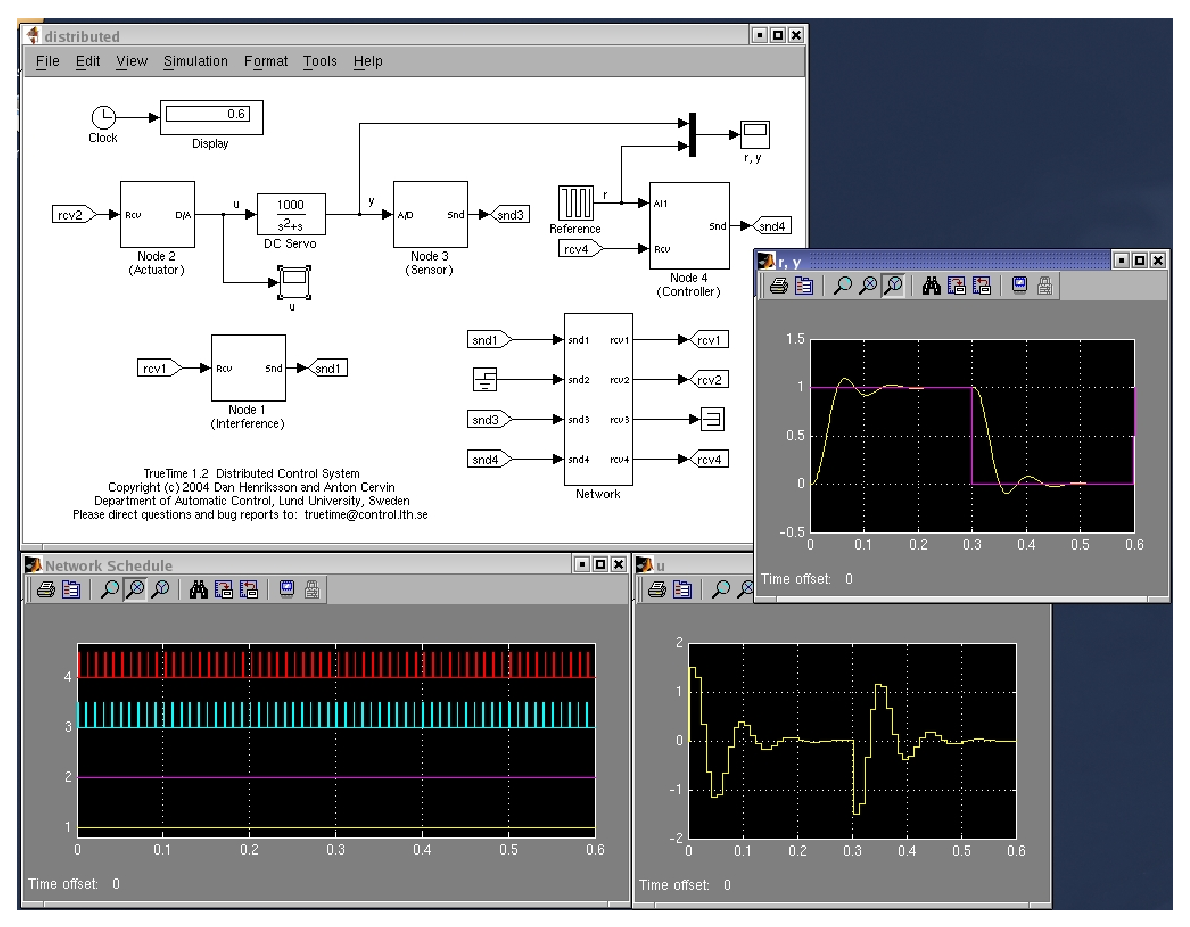
\includegraphics[scale=.6]{dist.ps}
  \end{center}
  \caption{The \textsc{TrueTime} model of the networked control system.}
  \label{fig:dist}
\end{figure}

\subsubsection{Simulations}
The Simulink model is called \texttt{networked.mdl} and is given in
Figure~\ref{fig:dist}. Open the Simulink model and try the following

\begin{itemize}
\item Study the initialization scripts and code functions for the
  different nodes. The event-driven nodes contain interrupt handlers,
  which are activated as messages arrive over the network. The handler
  then triggers the task that will read and process the message.
\item Run a first simulation without disturbing traffic and without
  interference in the controller node. This is obtained by setting the
  variable \texttt{BWshare} in the code function of the interfering
  node (\texttt{interfcode.m}) to zero, and by commenting out the
  creation of the task \texttt{'dummy'} in \texttt{controller\_init}.
  In this case we will get a constant round-trip delay and
  satisfactory control performance. Study the network schedule
  (high=sending, medium=waiting, low=idle) and the resulting control
  performance.
\item Switch on the disturbing node and the interfering task in the
  controller node. Set the variable \texttt{BWshare} to the percentage
  of the network bandwidth to be used by the disturbing node. Again
  study the network schedule and the resulting control performance.
  Experiment with different network protocols and different scheduling
  policies in the controller node.
\end{itemize} 


% \subsection{Deadline Overrun Handling}
% \label{sec:overrun}

% \subsubsection{Introduction} 
% This example will show how to use the \textsc{TrueTime} overrun
% handling functionality. \textsc{TrueTime} provides two types of
% overrun handlers; deadline and worst-case execution time overrun
% handlers. The example again considers PID-control of the DC-servo
% described by Equations (\ref{eq:servo}) and (\ref{eq:ctrl}). However,
% now the controller task is having a stochastically varying execution
% time that occasionally will exceed the sampling interval. Two
% approaches to deal with the period overruns are evaluated in the
% simulation. The first allows the task to continue into next sample (no
% overrun handler is attached), whereas the second uses an overrun
% handler that terminates the current job if the deadline is exceeded.
% The files are found in the directory \texttt{\$DIR/examples/overrun}.

% \subsubsection{Simulations}
% Open the Simulink model \texttt{overrun.mdl} and try the following

% \begin{itemize}
% \item Study the code function \texttt{pidcode.m}, then run a
%   simulation. The period of the controller task is $6$~ms, and the
%   execution time is modeled as $C = 5 + U(0,2)$~ms. Consequently, the
%   task will experience overruns. The bad control performance is due to
%   the long delays and the sampling period jitter induced by the
%   overruns.
% \item Uncomment the last two lines of the initialization file
%   (\texttt{overrun\_init.m}). This will create an interrupt handler
%   and attach it to the controller task as a deadline handler. Study
%   the code executed by the overrun handler (\texttt{hdlcode.m}).
% \item Run a simulation to evaluate the performance obtained by terminating
%   jobs at the deadline (is this a good approach?). Studying the control 
%   signal, one can notice that it often remains constant over several 
%   samples.
% \end{itemize} 

% \subsection{Task Synchronization Using Monitors}

% \subsubsection{Introduction}
% This example shows how to use monitors to obtain mutual exclusion in
% \textsc{TrueTime}. A cascaded controller for a ball-and-beam process
% is implemented using separate tasks for the two loops in the cascade.
% The output from the outer controller is used as input to the inner
% controller and is communicated using a global variable. This variable
% is a shared resource, and mutual exclusion is achieved by a
% \textsc{TrueTime} monitor. The files are found in the directory
% \texttt{\$DIR/examples/synch}.

% \subsubsection{Process and Controller}

% \begin{figure}[tbp]
%   \centerline{
%     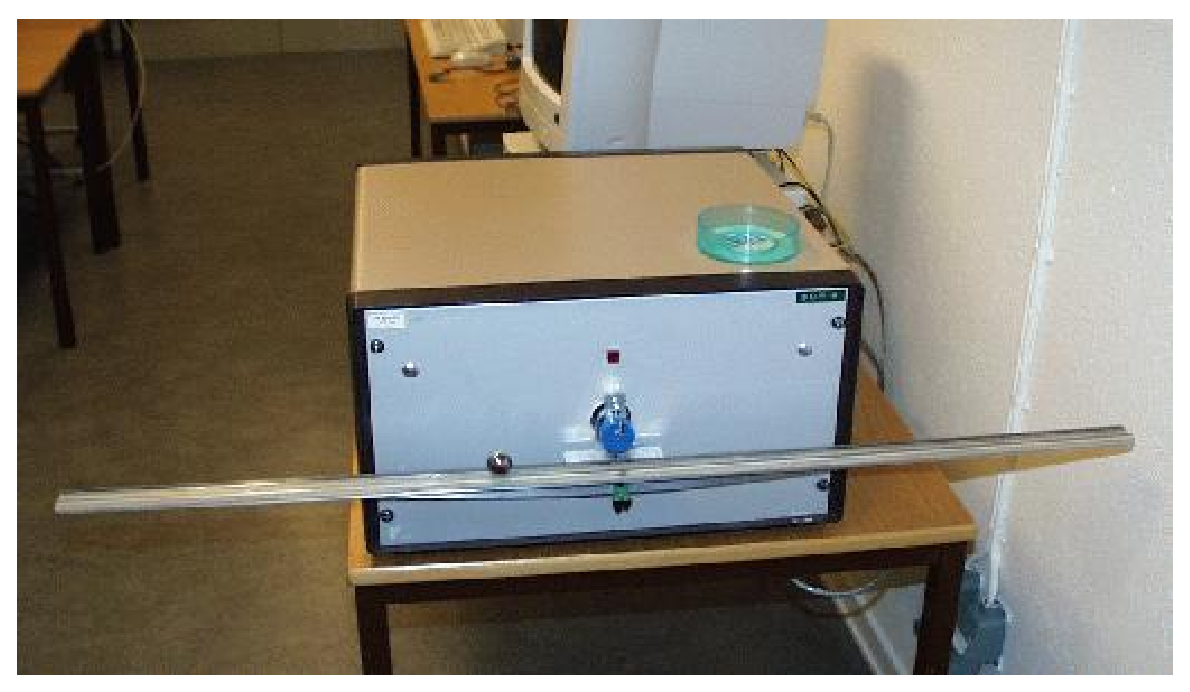
\includegraphics[scale=0.6]{bom.ps}
%     }
%   \caption{The ball and beam laboratory process.}
%   \label{fig:bab}
% \end{figure}

% The ball and beam laboratory process is shown in
% Figure~\ref{fig:bab}. The horizontal beam is controlled by a motor,
% and the objective is to balance the ball along the beam. The
% measurement signals from the system are the beam angle, denoted by
% $\phi$, and the ball position on the beam, denoted by $x$. A
% linearized model of the system is given by

% \begin{equation}
% \label{eq:bab}
% G(s) = G_{\phi}(s)G_x(s)
% \end{equation}
% where
% \begin{equation}
% G_{\phi}(s) = \frac{k_{\phi}}{s}
% \end{equation}
% is the transfer function between the motor input and the beam angle,
% and
% \begin{equation}
% G_{x}(s) = - \frac{k_{x}}{s^2}
% \end{equation}
% is the transfer function between the beam angle and the ball position.
% The gains of the systems are given by $k_{\phi} \approx 4.4$ and $k_x
% \approx 9$. 

% The cascaded controller is shown in Figure~\ref{fig:cascade}. The
% outer controller is a PID-controller (implemented according to
% Equation (\ref{eq:ctrl})) and the inner controller is a
% simple P-controller.

% \begin{figure}
% \vspace*{1em}
% \small
%   \centerline{
%     \psfrag{pos}[][]{$x_r$}
%     \psfrag{ang}[][]{$\phi_r$}
%     \psfrag{C1}[][]{PID-ctrl}
%     \psfrag{C2}[][]{P-ctrl}
%     \psfrag{G1}[][]{$G_{\phi}(s)$}
%     \psfrag{G2}[][]{$G_{x}(s)$}
%     \psfrag{x}[][]{$x$}
%     \psfrag{p}[][]{$\phi$}
%     \psfrag{u}[][]{$u$}
%     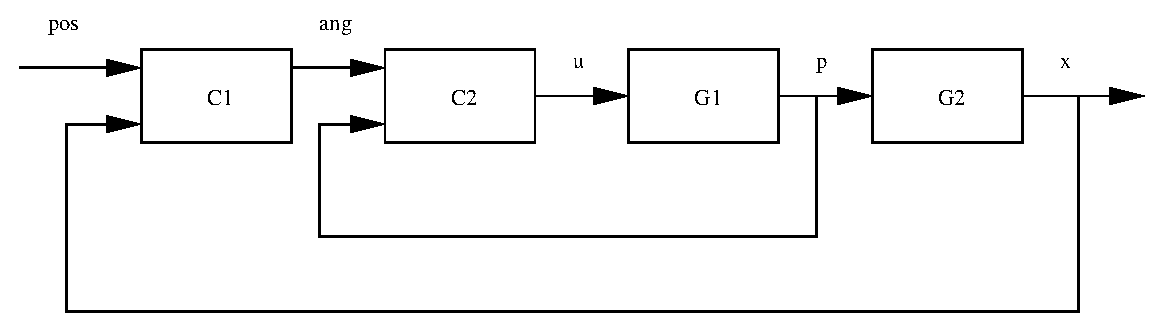
\includegraphics[scale=.5]{cascade.eps}
%     }
%   \caption{The cascaded controller structure for the ball and beam process.}
%   \label{fig:cascade}
% \end{figure}

% \begin{figure}[tbp]
%   \begin{center}
%     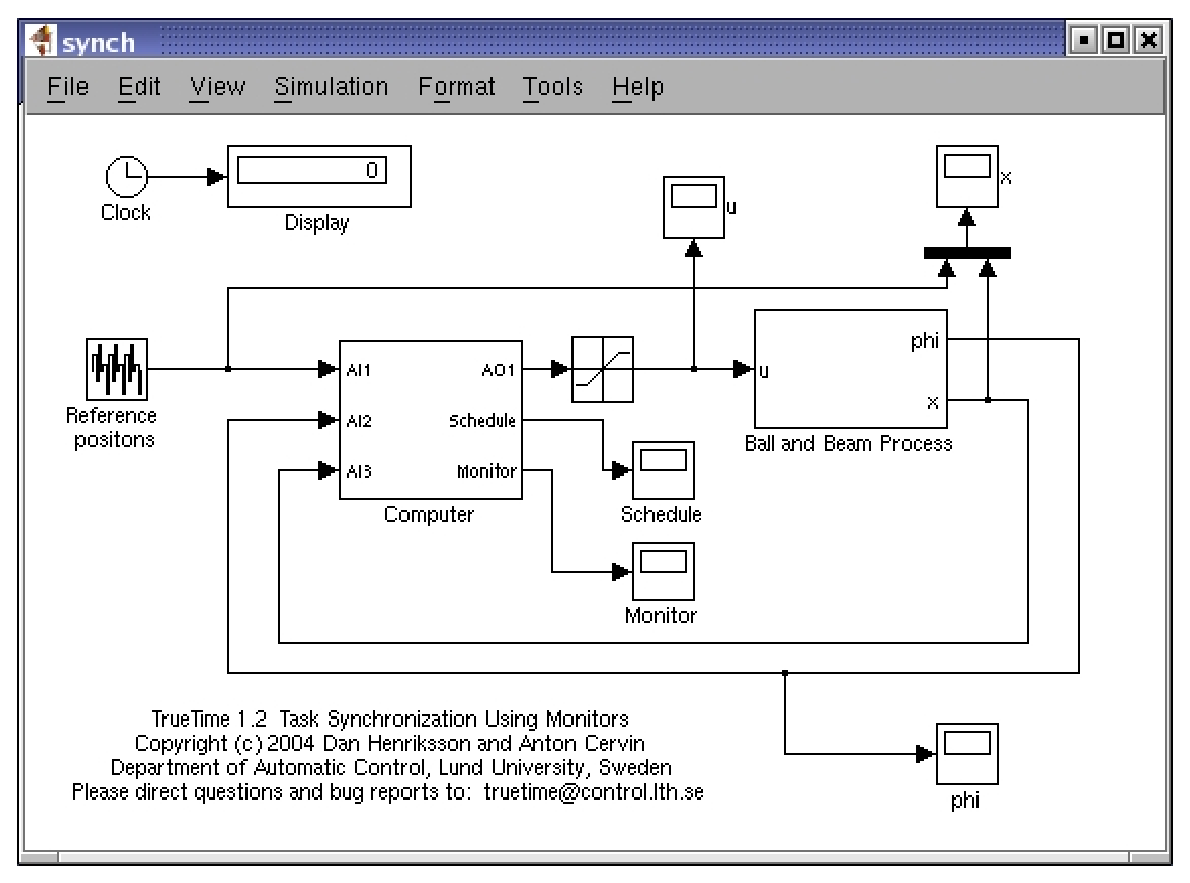
\includegraphics[scale=.45]{synch.ps}
%   \end{center}
%   \caption{The \textsc{TrueTime} model of the ball and beam system.}
%   \label{fig:synch}
% \end{figure}

% \subsubsection{Simulations}
% The Simulink model is called \texttt{synch.mdl} and is given in
% Figure~\ref{fig:synch}. Open the Simulink model and try the following

% \begin{itemize}
% \item Study the initialization function (\texttt{synch\_init.m}). This
%   creates two tasks for the outer and inner loop, respectively. A
%   global variable, \texttt{outerU}, is used for task communication.
%   This variable is the output from the outer controller (thus its
%   name) and is used as reference for the inner controller (it is
%   denoted $\phi_r$ in Figure~\ref{fig:cascade}). Finally, a
%   \textsc{TrueTime} monitor is created.
% \item Study the code functions for the controller tasks
%   (\texttt{outercode.m} and \texttt{inner} \texttt{code.m}). To ensure
%   that no further instructions are executed in the case that
%   \texttt{ttEnterMonitor} fails, this primitive needs to be called
%   from its own segment (since all code of a \textsc{TrueTime} segment
%   is executed at once before scheduling decisions are made). The same
%   holds for \texttt{ttExitMonitor} to make sure that no further code
%   is executed in the case a context switch will occur when the monitor
%   is released.
% \item Run a simulation and study the monitor graph. This graph displays when 
%   the various tasks have been holding the monitor during the simulation.
% \item Try modifying the periods of the tasks to change the phasing and to see 
%   which loop that is most sensitive to slower sampling.  
% \end{itemize} 

%\section{Implementing Higher Level Network Protocols}

%The \textsc{TrueTime} network block simulates the basic properties of
%standard MAC (media access control) layer protocols. These protocols
%constitute the link layer in the Internet protocol stack, and are
%typically implemented in a network interface card, see \cite{kur_ross}. 

%It is, however, straightforward to also implement higher level
%protocols using \textsc{TrueTime}. Transport layer protocols, such as
%TCP and UDP, are usually implemented in software in the end systems,
%and may be emulated directly in the various \textsc{TrueTime} computer
%nodes using dedicated tasks or interrupt handlers.

%A simple TCP implementation will be outlined below. In the simulation
%it is possible to specify TCP specific parameters such as sizes of the
%buffers at the receiving and sending ends, receive windows, maximum
%segment size (MSS), and acknowledgment time-outs. The receive windows
%are used to implement flow control. The window gives an indication of
%the free buffer space at the receiving side, and dictates how much
%data that can be transmitted on that specific connection. The window
%size is constantly updated by the receiving node, as messages are
%being read from the application layer. This information is sent back
%to the sender with each acknowledgment. No congestion control is
%implemented.

%\subsection{Opening a TCP Connection}

%Since TCP is connection-oriented, a socket connection must be
%established before two nodes can start sending and receiving messages.
%When a connection is set up, sending and receiving buffers are created
%at each end of the connection. Special \textsc{TrueTime} sending and
%receiving tasks are also associated with each connection. Using tasks
%for the processing of incoming and outgoing TCP packets, it is
%possible to simulate overhead in the TCP layer. The functionality
%performed by these tasks will be described below.

%\subsection{Sending a TCP Data Message}

%When sending a message over TCP it is divided in segments of size MSS
%which are sent in sequence to the receiving end, where the message is
%recreated. In addition to the data, each TCP data segment includes a
%header containing fields for source and destination identifiers,
%sequence number, acknowledgment number, and window size. 

%When a segment is transmitted, a timer is created. If no
%acknowledgment has been received at the expiry of the timer, the
%segment is resent. The sending of a message is summarized in
%pseudo-code in Listing~\ref{list:TCPsend}.

%\begin{listing}[tb]\small
%\caption{Pseudo code for the sending of a TCP data message.}
%\label{list:TCPsend}
%\vspace{3mm}
%\hrule
%\begin{verbatim}
%  double TCPSend_code(int seg, void *data) {

%    i = 0;
%    ready = false;

%    // Send all segments in send buffer and set up timers
%    while (!ready) {
%      // Take next segment from send buffer
%      segment = sendBuffer->get(i);
%      // Send if window allows
%      if (segment->seqNbr <= sendWindow) {
%        segment->ackNbr = lastRcv;
%        ttSendMsg (segment->destination, segment, segment->size);
%        time = ttCurrentTime() + TIMEOUT;
%        Create timer for resending at t = time;
%      } else {
%        // Send window full, can not send
%        ready = true;
%      }
%      // Increase buffer index
%      i++;
%      if (i == sendBuffer->currentSize()) {
%        // No more segments in send buffer
%        ready = true;
%      }
%    }
%    return i * SND_OVERHEAD_TIME; // task execution time
%  }
%\end{verbatim}
%\hrule
%\end{listing}

%\subsection{Receiving a TCP Data Segment}

%When a TCP segment arrives at a node, it is handled by a receiving
%task. An incoming TCP segment may be either a data segment or an
%acknowledgment of a previously transmitted segment. 

%In the first case, it is checked if all preceding segments have been
%received. In this case the data is put in the receive buffer,
%otherwise the segment is discarded. An acknowledgment, with the latest
%received sequence number, is then sent back to the source node. When
%all segments of a message have been received, the application layer is
%notified.

%In the case that the incoming segment is a first-time acknowledgment,
%it works as a cumulative acknowledgment of all previous data, and the
%corresponding timers are removed. If we get a duplicate
%acknowledgment, however, this indicates that segments in between have
%been lost. In this case a fast re-transmit is performed, before the
%actual expiry of the timer of the segment. The implementation is
%summarized in pseudo-code of Listing~\ref{list:TCPrcv}.

%\begin{listing}[tb]\small
%\caption{Pseudo code for the receiving of a TCP data segment.}
%\label{list:TCPrcv}
%\vspace{3mm}
%\hrule
%\begin{verbatim}
%  double TCPReceive_code(int seg, void *data) {
  
%    // Get segment from data link layer
%    segment = ttGetMsg();

%    if (segment contains data) {
%      if (segment->seqNbr == lastRcv) {
%        // have got all previous segments, put in buffer
%        rcvBuffer->put(segment);
%        lastRcv = segment->seqNbr + segment->size;
%        Increase size of receive window;        
%      } else {
%        // Out-of-order segment, ignore
%      }
%      // Send Ack
%      ack->seqNbr = -1;
%      ack->ackNbr = lastRcv;
%      ack->window = rcvWindow;
%      ack->source = segment->destination;
%      ack->destination = segment->source;
%      ttSendMsg(ack->destination, ack, ACKSIZE);
%    } else {
%      // We received an acknowledgement segment
%      sendWindow = segment->window;
%      if (segment->ackNbr > lastAck) {
%         // new Ack
%         lastAck = segment->ackNbr;
%         Remove timeout timers;
%         Delete segments from send buffer;
%      } else {
%        // same Ack as previously received
%        Packets was lost, fast re-transmit;
%      }
%    }
%    return RCV_OVERHEAD_TIME; // task execution time
%  }
%\end{verbatim}
%\hrule
%\end{listing}

%\subsection{Communicating with the Application Layer}

%The sending TCP task is triggered from the application layer when a
%user wants to send a message on the specific connection. Then the
%message is divided in segments and stored in the send buffer for
%subsequent transmission to the receiver. When the message is later
%resembled at the receiving end the application layer is notified and
%the message can be read from the receive buffer. \textsc{TrueTime}
%events can be used to synchronize the application tasks and the TCP
%receive tasks, whereas the sending of a TCP message should be a
%non-blocking operation.

\vspace{1em}
\subsection{Wireless Control System with Automatic Gain Control}
\label{sec:wireless}

\subsubsection{Introduction}
This example shows networked control of a DC-servo described by
Equation~(\ref{eq:servo}) using
communication over a wireless network. The example also shows how to
simulate power consumption and how to use the battery block. The model
contains two computer nodes located 20 m apart, each represented by a
\textsc{TrueTime} kernel and battery block. A time-driven sensor/actuator node samples the
process periodically and sends the samples over the network to the
controller node. The control task in this node calculates the control
signal and sends the result back to the sensor/actuator node, where it
is actuated. The wireless communication link is at the same time
subject to a simple power control scheme. Power control tasks running
in both the sensor/actuator node and in the controller node
periodically send out ping messages to the other node to test the
channel transmission. If a reply is received, the channel is assumed
to be good and the transmission power is lowered. If on the other hand
no reply is received, then the transmission power is considerably
increased until it saturates or a reply is received again. The files
are found in the directory \texttt{\$DIR/examples/wireless}.

\subsubsection{Simulations}
Open the model \texttt{wireless.mdl} to run the simulation. 

\begin{itemize}
\item Run a first simulation without modifying anything. Look at the plots
   showing the battery levels in the two nodes. Note that the power control
   scheme is not activated until ~2 seconds have elapsed. Also note how the 
   measured values at some times deviate more than usual from the reference
   values. This deviation is caused by the fact that it is possible to lose
   several consecutive sensor value readings when using the simple power 
   control that is implemented in the nodes.

\item Switch off the power control scheme in the controller node. This is done
   by commenting out the creation of the task {\tt power\_controller\_task} in 
   {\tt controller\_init}. Run the simulation again and now note that the power drain
   is constant in the controller node. This causes the battery to run out
   of energy and the control is lost.

\item Experiment with different network
   parameters and protocols and see how it affects the control
   behaviour. In this example, the kernel block is set to consume
   $10$ mW. This can easily be changed by using the command {\tt
     ttSetKernelParameter}. This command can also be used to set the
   CPU scaling factor to enable Dynamic Voltage Scaling.

\end{itemize}

% \begin{figure}[tbp]
%   \centerline{
%     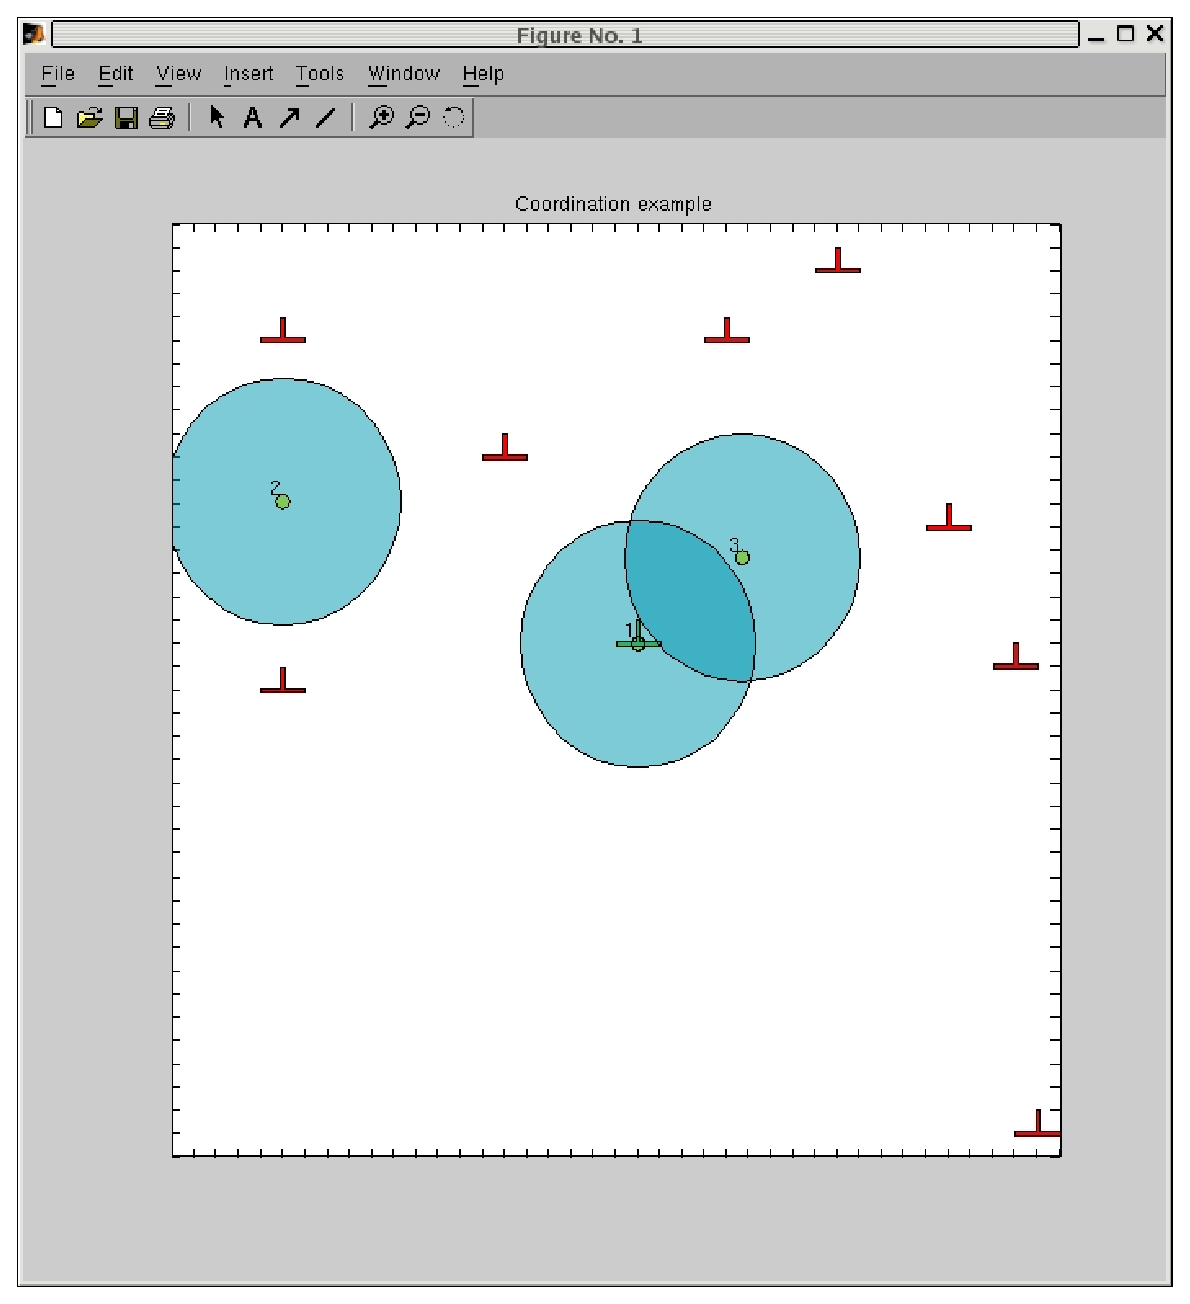
\includegraphics[scale=.26]{motes.ps}
%     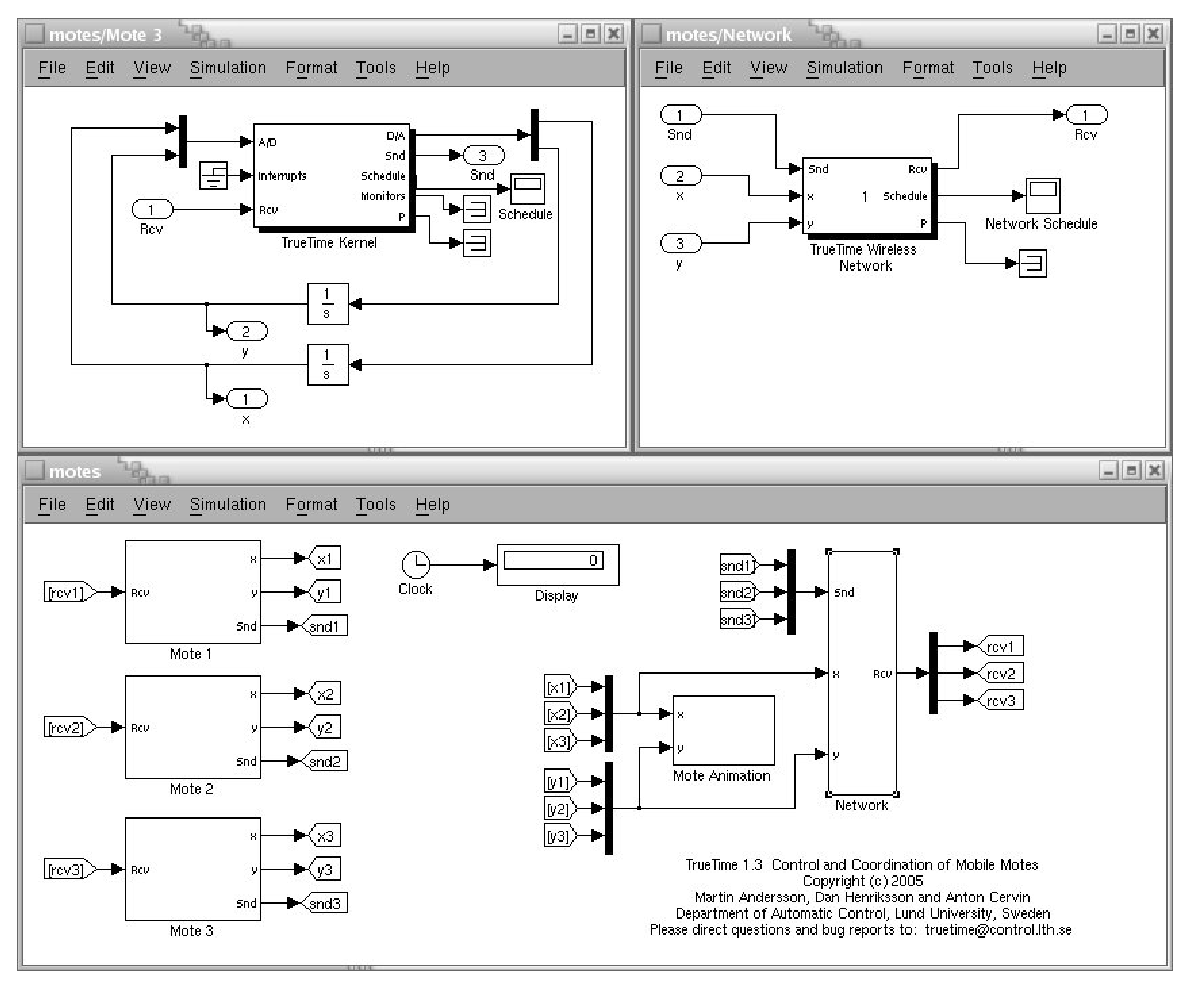
\includegraphics[scale=.45]{motes_mdl.ps}}
%   \caption{Visualisation of motes in Example~\ref{sec:motes}.}
%   \label{fig:motes}
% \end{figure}

% \subsection{Control and Coordination of Mobile Motes}
% \label{sec:motes}

% \subsubsection{Introduction}
% This example shows how to visualise the movements of dynamically
% moving motes using the built in functionality of matlab. The example
% consists of three motes, with dynamics in the {\tt x} and {\tt y}
% directions modeled using simple integrators. The motes are sent out on
% a mission which consists of visiting a number of checkpoints seen as
% red marks in the animation window in Figure~\ref{fig:motes}. In the
% window, the transmission range of the motes can be seen as large
% partly transparent coloured circles around the smaller coloured motes.
% The checkpoints should be visited at least once by some node in the
% group. When the motes are able to communicate, they tell each other
% where they are heading and share information on which nodes that have
% been visited by the group. Some of this information is visible as
% printouts during the execution. When a checkpoint has been visited it
% changes colour from green to red. The files are found in the directory
% \texttt{\$DIR/examples/motes}.

% \subsubsection{Simulations}
% Open the model \texttt{motes.mdl} to run the simulation. 

% \begin{itemize}
% \item Run {\tt init} to set up the data structures before you run the simulation.
% \item Run the simulation to see the animation. If you are interested
%   in building your own custom animation, look at the file
%   \texttt{moteanimation.m}
%   where the {\tt patch} command is used to paint the initial
%   picture of every mote. These pictures are then moved with the {\tt
%     set} command using the {\tt XData} and {\tt YData} parameters.
% \end{itemize}

% The motes operate according to the following algorithm:
% \begin{enumerate}
% \item Read new network messages containing information of:\\
%   \hspace*{5mm} visited nodes\\
%   \hspace*{5mm} target of the sending node
% \item If (someone has the same target as we do \&\& we
%   have the lowest priority),\\
%   \hspace*{5mm} then change target
% \item If (heading to a place that has already been visited),\\
%  \hspace*{5mm} then change target
% \item If (arrived at target)\\
%   \hspace*{5mm} then paint the target green \&\& change target
% \item Send new network messages to other nodes
% \end{enumerate}

\subsection{Wireless Ad-hoc Routing Using AODV}
\label{sec:AODV}

\subsubsection{Introduction}
The \textsc{TrueTime} wireless network simulates communication in an
ad-hoc network, i.e., no centralized access point or infrastructure
exists to coordinate the traffic across the network. In such networks
it is necessary to implement decentralized functionality to be able to
route the traffic over the network. This example describes a
\textsc{TrueTime} implementation of one such ad-hoc wireless routing
protocol. 

AODV \cite{per+roy99} stands for Ad-hoc On-Demand Distance Vector
routing and contrary to most routing mechanisms, it does not rely on
periodic transmission of routing messages between the nodes. Instead,
routes are created on-demand, i.e., only when actually needed to send
traffic between a source and a destination node. This leads to a
substantial decrease in the amount of network bandwidth consumed to
establish routes. Below follows a brief description of the
functionality of AODV. For a complete definition of the AODV protocol,
see \cite{AODVrfc}.

AODV uses three basic types of control messages in order to build and
invalidate routes: route request (RREQ), route reply (RREP), and route
error (RERR) messages. These control messages contain source and
destination sequence numbers, which are used to ensure fresh and
loop-free routes.

A node that requires a route to a destination node initiates route
discovery by broadcasting an RREQ message to its neighbors. A node
receiving an RREQ starts by updating its routing information backwards
towards the source. If the same RREQ has not been received before, the
node then checks its routing table for a route to the destination. If
a route exists with a sequence number greater than or equal to that
contained in the RREQ, an RREP message is sent back towards the
source. Otherwise, the node rebroadcasts the RREQ. When an RREP has
propagated back to the original source node, the established route may
be used to send data. Periodic hello messages are used to maintain
local connectiviy information between neighboring nodes. A node that
detects a link break will check its routing table to find all routes
which use the broken link as the next hop. In order to propagate the
information about the broken link, an RERR message is then sent to
each node that constitute a previous hop on any of these routes.

The files for this tutorial example are found in the directory
\texttt{\$DIR/examples/AODV}. All nodes are initialized using the same
initialization script, \texttt{node\_init.m}. Two \textsc{TrueTime}
tasks are created in each node to handle AODV send and receive
actions, respectively. The AODV send task is activated from the
application code as a data message should be sent to another node in
the network. The AODV receive task handles incoming AODV control
messages and forwarding of data messages. Communication between the
application layer and the AODV layer is handled using
\textsc{TrueTime} mailboxes.

The AODV send task (\texttt{AODVsendcode.m}) operates according to the
following code:

\begin{small} 
\begin{verbatim}
  IF (data message received from application)
     check the routing table for a route to the destination;
     IF (a valid route exists)
        forward data message to next hop on route;
        update expiry time of route entry;
     ELSE
        initiate route discovery by broadcasting RREQ message;
        buffer data message until route has been established;
     END
  ELSE IF (notified of established new route)
     send all buffered data messages to destination
  END
\end{verbatim}
\end{small} 

The AODV receive task (\texttt{AODVrcvcode.m}) performs the following:

\begin{small} 
\begin{verbatim}
  IF (receiving data message)
     update expiry timer for reverse route entry to source;
     IF (this node is the destination)
        Pass data message to application;
     ELSE
        forward data message to next hop on route;
        update expiry timer of route entry;
     END
  ELSE
     SWITCH message_type
        CASE RREQ:
           IF (first time this RREQ is received)
              enter RREQ in cache;
              create or update route entry to source;
              check the routing table for a route to the destination;
              IF (a route exists)
                 send RREP message back towards source;
              ELSE
                 update and rebroadcast the RREQ;
              END
           END
        CASE RREP:
           check the routing table for a route to the destination;
              IF (no route exists)
                 create route entry to destination;
              ELSE IF (route entry exists but should be updated)
                 update route entry to destination;
              END
              IF (this node is the original source)
                 notify the AODV send task about the new route;
              ELSE IF (route to destination was created or updated)
                 update reverse route entry towards source;
                 propagate RREP to next hop towards source;
              END
        CASE RERR:
              find and invalidate all affected route entries;
              propagate the RERR to all previous hops on the routes;
     END
  END
\end{verbatim}
\end{small} 

Each node also contains a periodic task (\texttt{hellocode.m}),
responsible for broadcasting hello messages and determine local
connectivity based on hello messages received from neighboring nodes.
Finally, each node has a task to handle timer expiry of route entries
(\texttt{expcode.m}).



\subsubsection{Simulations}

Open the model \texttt{AODV.mdl} to run the simulation. 

\begin{itemize}
\item The simulation example consists of seven nodes. Choose the option
  Update Diagram in the Edit menu to bring up an animation window of
  the simulation. This will show the original positions of the seven
  nodes and their respective signal reach.

\item Run a simulation. In the simulation scenario, the left-most node
  (node $1$) sends data periodically to node $7$ with period $0.5$.
  The initial route that is established is $1 \rightarrow 3
  \rightarrow 5 \rightarrow 7$. At time $t=3$, node $5$ starts to move
  which eventually leads to the route breaking. At time $t=10$, node
  $6$ repairs the route by moving in between node $4$ and $7$. The
  printouts in the Matlab command window describe the actions in the
  AODV layer in more detail. Also study the global variable
  \texttt{routing\_table}. 

\item Open and examine the file \texttt{initsim.m}. This file
  initializes the global variables used in the simulation, e.g., the
  routing table and the node positions. By changing the variable
  \texttt{verbose} from $0$ to $1$ even more detailed AODV
  information will be displayed when the simulation is run.

\item The global variables \texttt{sent} and \texttt{received} show
  the data that is sent (by node $1$) and received (by node $7$) in
  the simulation. Examine the lengths of these vectors to determine
  how many messages that where lost due to the delay in detecting and
  propagating the information about the broken link back to the source
  node. (Answer: The messages sent at times $8.0002$, $8.5002$, and
  $9.0002$ are lost.)

\item The hello interval determines who fast the network will respond
  to broken links (and also the bandwidth overhead). Try changing the
  AODV parameter \texttt{HELLO\_INTERVAL} (both in \texttt{initsim.m}
  and \texttt{node\_init.m}) to decrease the number of lost data
  messages. In this case only two messages are lost.

\end{itemize}

\subsection{Mote Soccer}

This largely undocumented example features a slighly more complex
simulation set-up where ten mobile robots are playing soccer. The
robots and the ball are animated during the simulation, see
Figure~\ref{fig:soccer}. 
\begin{figure}
  \centerline{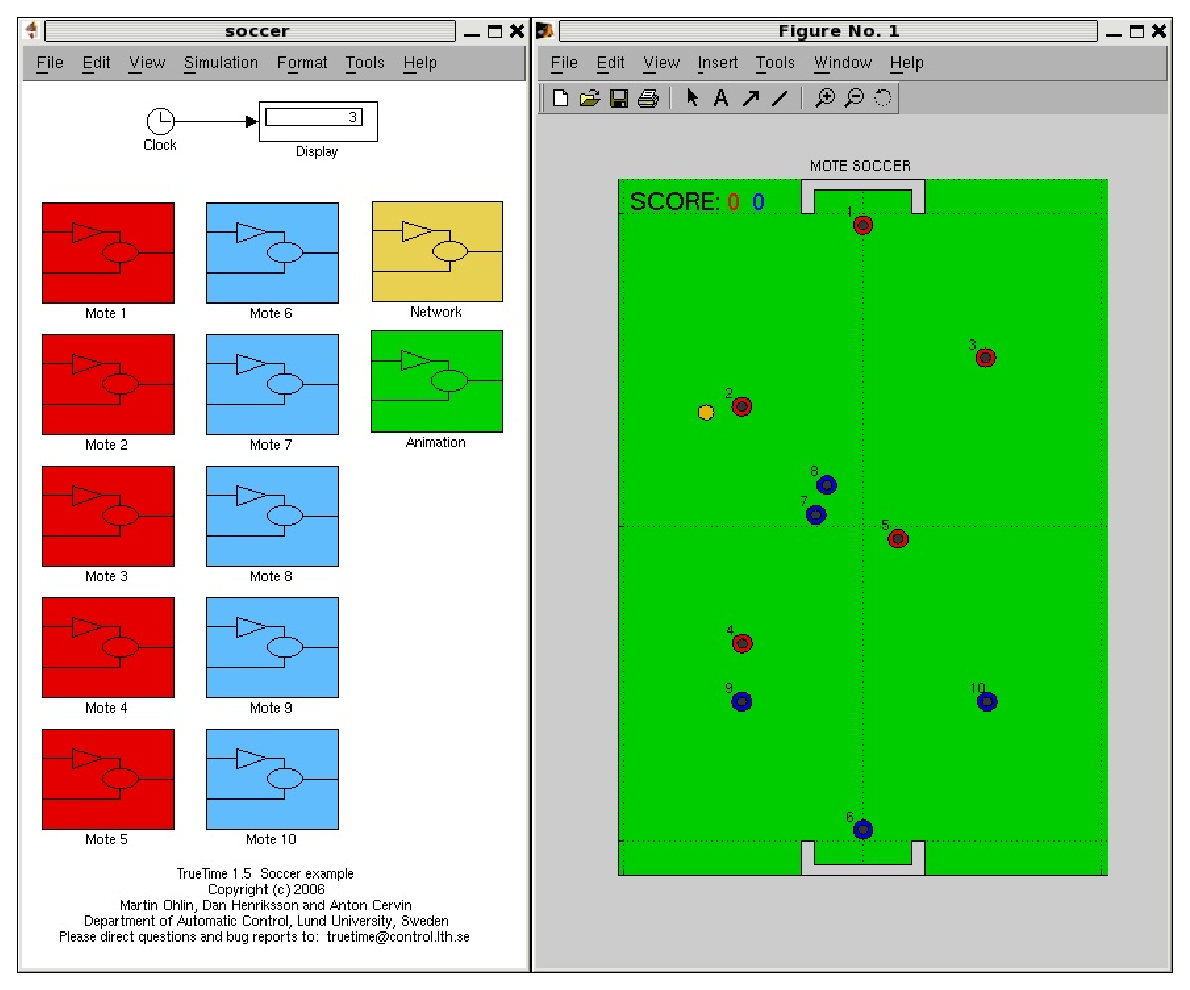
\includegraphics[width=0.9\hsize]{soccer.ps}}
  \caption{Mote soccer.}
  \label{fig:soccer}
\end{figure}
The simulation files are found in the directory
\texttt{\$DIR/examples/soccer}.

Each mobile robot (mote) is modeled using a kernel block and two
integrators representing the $x$ and $y$ coordinates of the robot. The
ball is modeled as a forth-order system (an integrator plus damping in
each direction) implemented in an S-function ({\tt ballmotion.m}).
This S-function also handles the player interaction with the ball. The
robots within each team communicate over the wireless network. The
goalkeeper is each team acts as the ``master'' and coordinates the
players. 

The mask of the network block is programmed to dynamically change the
contents of the underlying subsystem (study the initialization
commands). This is a very conventient feature when working with a
large number of network nodes.

% \subsection{The stand-alone network blocks}

% The two examples {\tt timetriggered.mdl} and {\tt eventtriggered.mdl}
% in the directory \texttt{\$DIR/examples/ttsendmsg}
% demonstrate how the new stand-alone network blocks can be used to
% simulate networked control loops, see Figure~\ref{fig:ttsendmsg}.
% \begin{figure}
%   \centerline{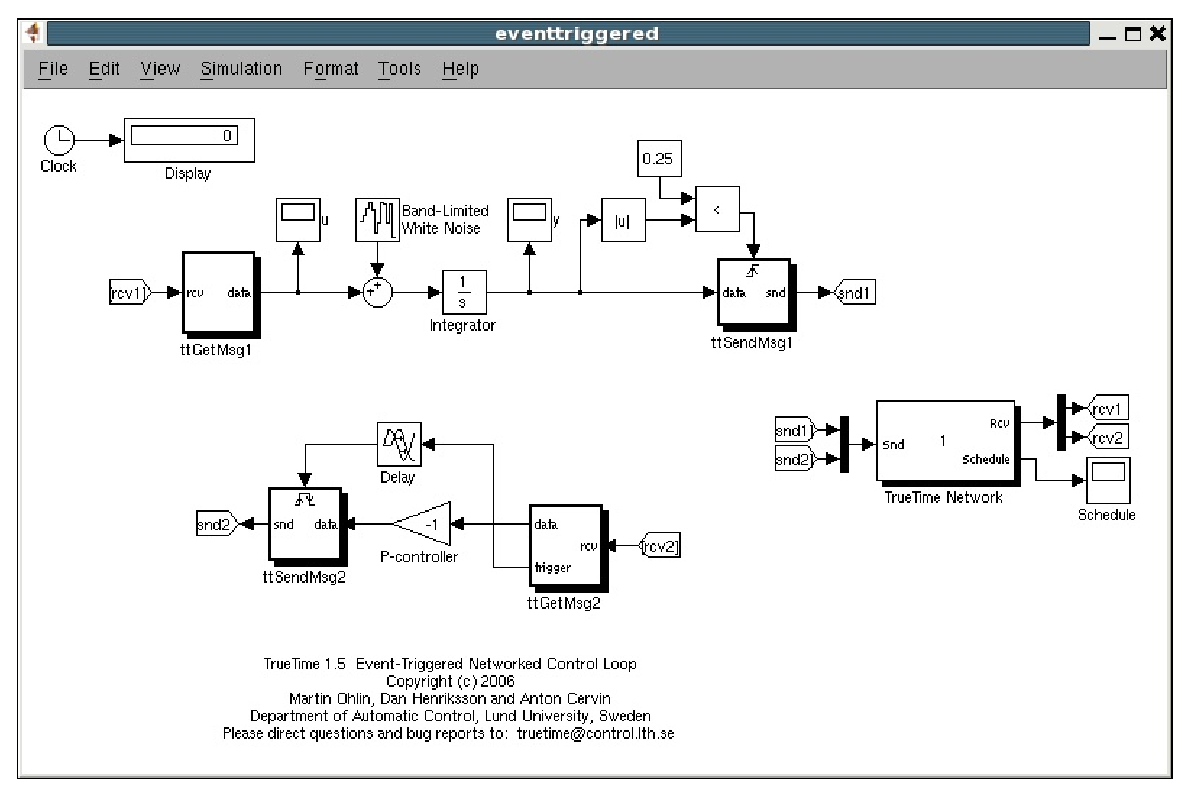
\includegraphics[width=0.9\hsize]{ttsendmsg.ps}}
%   \caption{Event-triggered networked control loop using the new
%     ttSendMsg/ttGetMsg stand-alone network blocks.}
%   \label{fig:ttsendmsg}
% \end{figure}

% In the time-triggered example, the send blocks are triggered by pulse
% generators with a period of 0.1~s. The pulse generator of the second
% node has an offset (phase delay) of 0.05~s. A simple P-controller is
% used to stabilize the integrator which is disturbed by white noise.

% In the event-triggered example, the send block at the process is
% triggered whenever the magnitude of the process output exceeds 0.25.
% The controller at the reciever is also event-triggered, and in turn
% triggeres the second send block with a delay of 0.001~s. The control
% signal at the second receiver (at the process) is held between
% updates. It is seem that this set-up gives almost as good performance
% as the time-triggered scheme, while the network utilization is much
% lower.


\section{Kernel Implementation Details}

This section will give a brief description of the implementation of
the \textsc{TrueTime} kernel. The main data structures will be
described as well as the kernel implementation. It will also be
described how the event-based kernel simulation is achieved in
Simulink, using the zero-crossing detection mechanism.

\subsection{Kernel Data Structures}

The main data structure of the \textsc{TrueTime} kernel is a C++ class
called \texttt{RTsys}, see \texttt{\$DIR/kernel/ttkernel.h}. An
instance (\texttt{rtsys}) of this class is created in the
initialization step of the kernel S-function. The \texttt{rtsys}
object is stored in the \texttt{UserData} field of the kernel block
between simulation steps. Among others, the \texttt{RTsys} class
contains the following attributes:

\begin{small}
\begin{verbatim}
class RTsys {
 public:
  double time;              // Current time in simulation
  
  double* inputs;           // Vector of input port values
  double* outputs;          // Vector of output port values

  Task* running;            // Currently running task

  List* readyQ;   // usertasks and handlers ready for execution, prio-sorted
  List* timeQ;    // usertasks and timers waiting for release, time-sorted

  List* taskList;    // A list containing all created tasks
  List* handlerList;
  List* monitorList;
  List* eventList;
  
  double (*prioFcn)(Task*); // Priority function
};
\end{verbatim}
\end{small}

The ready queue and time queue are sorted linked list. The elements in
the time queue (tasks and timers) are sorted according to release
times and expiry times. A timer in the time queue is actually
represented by its corresponding handler. The tasks in the ready queue
are sorted according to the priority function \texttt{prioFcn}, which
is a function that returns a (possibly dynamic) priority number from a
\texttt{Task} instance, see the description of
\texttt{ttInitKernel} in the command reference.

The \texttt{Task} class (\texttt{\$DIR/kernel/task.h}) inherits from
the \texttt{node} class of the linked list
(\texttt{\$DIR/kernel/linkedlist.h}) and contains the following basic
attributes:

\begin{small}
\begin{verbatim}
class Task : public Node {
 public:
  char* name;
  int segment;      // the current segment of the code function
  double execTime;  // the remaining execution time of the current segment
  
  void *data;       // task data (C++ case)
  char* dataMatlab; // name of global variable for task data (Matlab case)

  double (*codeFcn)(int, void*); // Code function (C++ case)
  char* codeFcnMatlab;  // Name of m-file code function (Matlab case)
};
\end{verbatim}
\end{small}

The \texttt{exectime} of the running task is updated each time the
kernel executes, see Listing~\ref{list:runkernel}. When it has reached
zero, the next segment of the code function is executed. The task data
in the Matlab case is represented as a name of a unique global
variable.  The code function of a task is represented either as a
function pointer in the C++ case or the name of a Matlab m-file.

User tasks and interrupt handlers are both subclasses to \texttt{Task}
and contain the attributes given below, among others. See
\texttt{\$DIR/kernel/usertask.h} and \texttt{\$DIR/kernel/handler.h}
for complete descriptions.

\begin{small}
\begin{verbatim}
class UserTask : public Task {
public:
  double priority; 
  double wcExecTime;
  double deadline;
  double absDeadline; 
  double release;   // task release time if in timeQ
  double budget;
  
  int state;  // Task state (IDLE; WAITING; SLEEPING; READY; RUNNING)
  
  double tempPrio;  // temporarily raised prio value 

  List *pending; // list of pending jobs

  InterruptHandler* deadlineORhandler; // deadline overrun handler
  InterruptHandler* exectimeORhandler; // execution-time overrun handler
  
  int nbrOfUserLogs;  // Number of user-created log entries 
  Log* logs[NBRLOGS]; 
  
  void (*arrival_hook)(UserTask*);  // hooks
  void (*release_hook)(UserTask*);
  void (*start_hook)(UserTask*);
  void (*suspend_hook)(UserTask*);
  void (*resume_hook)(UserTask*);
  void (*finish_hook)(UserTask*);
};
\end{verbatim}
\end{small}

The kernel implements priority inheritance to avoid priority
inversion. Therefore each task has a dynamic priority value that may
be raised while executing inside a monitor. Pending jobs are stored in
the job queue of the task sorted by release time. See
\texttt{\$DIR/kernel/log.h} for the contents of the \texttt{Log}
class.

\begin{small}
\begin{verbatim}
class InterruptHandler : public Task {
 public:
  double priority;
  
  int type;  // {UNUSED, OVERRUN, TIMER, NETWORK, EXTERNAL}

  UserTask *usertask; // if overrun handler to task

  Timer* timer;       // if associated with timer interrupt 

  Network* network;   // if associated with network receive interrupt

  Trigger* trigger;   // if associated with external interrupt
  int pending;        // list of pending invocations, if new external
                      // interrupt occurs before the old is served
};
\end{verbatim}
\end{small}

See the corresponding header files in \texttt{\$DIR/kernel} for the
specifications of the classes \texttt{Timer}, \texttt{Network}, and
\texttt{Trigger}. 

\subsection{Task Model}
\textsc{TrueTime} user tasks may be periodic or aperiodic. Aperiodic
tasks are triggered by the creation of task jobs, using the command
\texttt{ttCreateJob}. All pending jobs are inserted in a job queue of
the task sorted by release time. For periodic task (created by the
command \texttt{ttCreatePer\-iodicTask}), an internal timer is set up
to periodically create jobs for the task.

Apart from its code function, each task is characterized by a number of
attributes. The static attributes of a task include
\begin{itemize}
\item a relative deadline
\item a priority
\item a worst-case execution time
\item a period (if the task is periodic)
\end{itemize}
These attributes are kept constant throughout the simulation, unless
explicitly changed by the user (see \texttt{ttSetX} in the command
reference).

In addition to these attributes, each task job has dynamic
attributes associated with it. These attributes are updated by the
kernel as the simulation progresses, and include
\begin{itemize}
\item an absolute deadline
\item a release time
\item an execution time budget (by default equal to the worst-case
  execution time at the start of each task job)
\item the remaining execution time
\end{itemize}
These attributes (except the remaining execution time) may also be
changed by the user during simulation. Depending on the scheduling
policy, the change of an attribute may lead to a context switch. E.g.,
if the absolute deadline is changed and earliest-deadline-first
scheduling is simulated.

In accordance with \cite{rtsj2000} it is possible to associate two
interrupt handlers with each task: a deadline overrun handler
(triggered if the task misses its deadline) and an execution time
overrun handler (triggered if the task executes longer than its
worst-case execution time). These handlers can be used to experiment
with dynamic compensation schemes, handling missed deadlines or
prolonged computations. Overrun handlers are attached to tasks with
the commands \texttt{ttAttachDLHandler} and
\texttt{ttAttachWCETHandler}. See the tutorial example in
Section~\ref{sec:overrun} for an example on how to use overrun
handlers.

Furthermore, to facilitate arbitrary dynamic scheduling mechanisms, it
is possible to attach small pieces of code (\textit{hooks}) to each
task. These hooks are executed at different stages during the
simulation, as shown in Figure~\ref{fig:hooks}. Usually the arrival
and release of a task job coincide. The exception is when a job is
created while previous jobs have yet to finish. In that case, the
arrival hook is executed immediately (at the call of {\tt
  ttCreateJob}) and the release hook is called when the job is
subsequently released from the job queue.

The hooks can, e.g., be used to monitor different scheduling schemes
and keep track of context switches and deadline overruns. By default,
the hooks implement logging, simulation of context switching, and
contain code to trigger the worst-case execution time and deadline
overrun handlers possibly associated with the different tasks. For the
default hook implementation, see
\texttt{\$DIR/kernel/default} \texttt{hooks.cpp}.

\begin{figure}[tbp]
  \center
  \psfrag{tau}[][]{$\tau$}
  \psfrag{t}[][]{$t$}
  \small
  \psfrag{p3}[][]{\begin{tabular}{c}Arrival, Release\\[-0.3em]hooks\end{tabular}}
  \psfrag{p4}[][]{\begin{tabular}{c}Start\\[-0.3em]hook\end{tabular}}
  \psfrag{p5}[][]{\begin{tabular}{c}Suspend\\[-0.3em]hook\end{tabular}}
  \psfrag{p6}[][]{\begin{tabular}{c}Resume\\[-0.3em]hook\end{tabular}}
  \psfrag{p7}[][]{\begin{tabular}{c}Finish\\[-0.3em]hook\end{tabular}}

  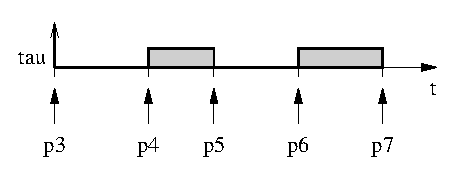
\includegraphics[scale=1.6]{hooks.eps}
  \caption{Scheduling hooks.}
  \label{fig:hooks}
\end{figure}
\vspace{2em}

\begin{listing}[tb]\small
\caption{Pseudo code for the \textsc{TrueTime} kernel function.}
\label{list:runkernel}
\vspace{3mm}
\hrule
\begin{verbatim}
double runKernel(void) {
  
  timeElapsed = rtsys->time - rtsys->prevHit; // time since last invocation
  rtsys->prevHit = rtsys->time;  // update previous invocation time
  nextHit = 0.0;

  while (nextHit == 0.0) {
    // Count down execution time for current task 
    // and check if it has finished its execution 
    if (there exists a running task) {
      task->execTime -= timeElapsed;
      if (task->execTime == 0.0) {
        task->segment++;
        task->execTime = task->codeFcn(task->segment, task->data);
        if (task->execTime < 0.0) { 
          // Negative execution time = task finished
          task->execTime = 0.0;
          task->segment = 0;
          Remove task from readyQ;
          task->finish_hook(task);
          if (job queue is non-empty)
            Release next job and execute release-hook ;
        }
      }
    } // end: counting down execution time of running task

    // Check time queue for possible releases (user tasks or timers)
    for (each task) {
      if ((release time - rtsys->time) == 0.0) {
        Move task to ready queue
      }
    } // end: checking timeQ for releases

    // Determine task with highest priority and make it running task
    newrunning = rtsys->readyQ->getFirst();
    oldrunning = rtsys->running;
    if (oldrunning is being suspended) {
      oldrunning->suspend_hook(oldrunning);
    }
    if (newrunning is being resumed or started) {
      if (newrunning->segment == 0) {
        newrunning->start_hook(newrunning);
      } else {
        newrunning->resume_hook(newrunning);
      }
    } // end: task dispatching
    
    // Determine next invocation of kernel function
    time1 = remaining execution time of current task;
    time2 = next release time of a task from the time queue
    nextHit = min(time1, time2);
  } // end: loop while nextHit == 0.0 
  return nextHit;
}
\end{verbatim}
\hrule
\end{listing}

\subsection{The Kernel Function}

The functionality of the \textsc{TrueTime} kernel is implemented by
the function \linebreak \texttt{runKernel} located in
\texttt{\$DIR/kernel/ttkernel.cpp}. This function manipulates the
basic data structures of the kernel, such as the ready queue and the
time queue, and is called by the Simulink call-back functions at
appropriate times during the simulation. See Section~\ref{sec:timing}
for timing implementation details.

It is also from this function that the code functions for tasks and
interrupt handlers are called. The kernel keeps track of the current
segment and updates it when the time associated with the previous
segment has elapsed. The hooks mentioned above are also called from
this function.

A simple model for how the kernel works is given by the pseudo code in
Listing~\ref{list:runkernel}. This code focuses on user tasks. See
\texttt{\$DIR/kernel/ttkernel.cpp} for the complete implementation.

\subsection{Timing}
\label{sec:timing}
The \textsc{TrueTime} blocks are event-driven and support external
interrupt handling. Therefore, the blocks have a continuous sample
time. Discrete (i.e., piecewise constant) outputs are obtained by
specifying {\tt FIXED\_IN\_MINOR\_STEP\_OFFSET}:
\begin{small}
\begin{verbatim}
  static void mdlInitializeSampleTimes(SimStruct *S) {

     ssSetSampleTime(S, 0, CONTINUOUS_SAMPLE_TIME);
     ssSetOffsetTime(S, 0, FIXED_IN_MINOR_STEP_OFFSET);
  }
\end{verbatim}
\end{small}

The timing of the block is implemented using a zero-crossing function.
As we saw above, the next time the kernel should wake up (e.g.,
because a task is to be released from the time queue or a task has
finished its execution) is denoted {\tt nextHit}. If there is no known
wake-up time, this variable is set to infinity. The basic structure of
the zero-crossing function is
\begin{small}
\begin{verbatim}
  static void mdlZeroCrossings(SimStruct *S) {

     Store all inputs;
        if (any interrupt input has changed value) {
           nextHit = ssGetT(S);
        }
     ssGetNonsampledZCs(S)[0] = nextHit - ssGetT(S);
  }
\end{verbatim}
\end{small}

This will ensure that {\tt mdlOutputs} executes every time an internal
or external event has occurred. Since several kernel and network
blocks may be connected in a circular fashion, {\em direct
  feedthrough} is not allowed. We exploit the fact that, when an input
changes as a step, {\tt mdlOutputs} is called, followed by {\tt
  mdlZeroCrossings}. Since direct feedthrough is not allowed, the
inputs may only be checked for changes in {\tt mdlZeroCrossings}.
There, the zero-crossing function is changed so that the next major
step occurs at the current time. This scheme will introduce a small
timing error ($<10^{-15}$~s).

The kernel function (\texttt{runKernel()}) is only called from {\tt
  mdlOutputs} since this is where the outputs (D/A, schedule, network)
can be changed. The timing implementation implies that {\em
  zero-crossing detection} must be turned on (this is default, and can
be changed under {\em Simulation Parameters/Advanced}).

\section{\textsc{TrueTime} Command Reference}
\label{sec:command_reference}
The available \textsc{TrueTime} commands are summarized in
Tables~\ref{table:commands}--\ref{table:prim}, and the rest of the
manual contains detailed descriptions of their functionality. The
commands are categorized according to their intended use ({\bf I};
initialization script, {\bf T}; task code function, and {\bf H};
interrupt handler code function). Note that the set and get primitives
are collected under the headings {\tt ttSetX} and {\tt ttGetX},
respectively.

By typing \texttt{help command}, where \texttt{command} is the name of
a \textsc{TrueTime} function, in the Matlab command window, the syntax
of the various \textsc{TrueTime} functions will be displayed.

\begin{table}
\caption{Commands used to create and initialize \textsc{TrueTime}
  objects, and to control the simulation.}
\label{table:commands}
\small
\begin{center}
\begin{tabularx}{\hsize}{|l|>{\raggedright\arraybackslash}X|}
\hline
Command & Description \\ \hline
{\tt ttInitKernel} & Initialize the kernel, specifying the scheduling policy. \\
{\tt ttGetInitArg (C++ only)} & Retrieve the init argument from the
block dialogue. \\
{\tt ttCreateTask} & Create an aperiodic task.\\
{\tt ttCreatePeriodicTask} & Create a periodic task. \\
{\tt ttCreateLog} & Create a log structure and specify data to log. \\
{\tt ttCreateHandler} & Create an interrupt handler. \\
{\tt ttCreateMonitor} & Create a monitor (mutex) for protection of
shared data. \\
{\tt ttCreateEvent} & Create an event (condition variable). \\
{\tt ttCreateMailbox} & Create a mailbox for inter-task communication. \\
{\tt ttCreateSempahore} & Create a counting semaphore. \\
{\tt ttCreateCBS} & Create a soft or hard constant bandwidth server. \\
{\tt ttNoSchedule} & Switch off the schedule plot for a specific
task or interrupt handler. \\
{\tt ttNonPreemptible} & Make a task non-preemptible. \\
{\tt ttAttachTriggerHandler} & Attach an interrupt handler to an external
trigger.\\
{\tt ttAttachNetworkHandler} & Attach an aperiodic task or interrupt handler 
to a network interface.\\
{\tt ttAttachDLHandler} & Attach a deadline overrun handler to a task.
\\ 
{\tt ttAttachWCETHandler} & Attach a worst-case execution time overrun
interrupt handler to a task. \\
{\tt ttAttachHook (C++ only)} & Attach a kernel scheduling hook to a task. \\ 
{\tt ttAttachCBS} & Attach a task to a constant bandwidth server. \\ 
{\tt ttAbortSimulation} & Abort the simulation. \\ 
\hline
\end{tabularx}
\end{center}
\end{table}

\enlargethispage{1em}

\begin{table}[htbp]
\caption{Commands used to set and get task or kernel attributes.}
\small
\label{table:getset}
\begin{center}
\begin{tabularx}{\hsize}{|l|>{\raggedright\arraybackslash}X|}
\hline
Command & Description \\ \hline
{\tt ttSetPeriod} & Set the period of a periodic task. \\
{\tt ttSetDeadline} & Set the relative deadline of a task. \\
{\tt ttSetPriority} & Set the priority of a task. \\
{\tt ttSetWCET} & Set the worst-case execution (maximum budget) time of a task. \\
{\tt ttSetData} & Update the local memory data structure of a task. \\
{\tt ttSetAbsDeadline} & Set the absolute deadline of the current job. \\
{\tt ttSetBudget} & Set the execution time budget of the current job. \\
{\tt ttSetUserData} & Set arbitrary kernel user data (C++ only). \\
{\tt ttGetPeriod} & Get the period of a periodic task. \\
{\tt ttGetDeadline} & Get the relative deadline of a task. \\
{\tt ttGetPriority} & Get the priority of a task. \\
{\tt ttGetWCET} & Get the worst-case execution time of a task. \\
{\tt ttGetData} & Retrieve the local memory data structure of a task. \\
{\tt ttGetRelease} & Get the release time of the current job. \\
{\tt ttGetAbsDeadline} & Get the absolute deadline the current job. \\
{\tt ttGetBudget} & Get the execution-time budget of the current job. \\
{\tt ttSetUserData} & Set the kernel user data (C++ only). \\
{\tt ttGetUserData} & Get the kernel user data (C++ only). \\
{\tt ttSetCBSParameters} & Set the parameters of a constant bandwidth server. \\
\hline
\end{tabularx}
\end{center}
\end{table}

\begin{table}[htbp]
\caption{Real-time primitives.}
\label{table:prim}
\small
\begin{center}
\begin{tabularx}{\hsize}{|l|>{\raggedright\arraybackslash}X|}
\hline
Command & Description \\ \hline
{\tt ttCreateJob} & Create a job of a task. \\
{\tt ttKillJob} & Kill the running (ready) job of a task, if any. \\
{\tt ttEnterMonitor} & Enter a monitor (blocking). \\
{\tt ttExitMonitor} & Exit a monitor. \\
{\tt ttWait} & Wait for an event (blocking). \\
{\tt ttNotify} & Notify the highest-priority task waiting for an event. \\
{\tt ttNotifyAll} & Notify all tasks waiting for an event. \\
{\tt ttLogStart} & Start a timing measurement for a log. \\
{\tt ttLogStop} & Stop a timing measurement and save in the log. \\
{\tt ttLogNow} & Log the current time. \\
{\tt ttLogValue} & Log a scalar value. \\
{\tt ttTryPost} & Post a message to a mailbox (non-blocking). \\
{\tt ttTryFetch} & Fetch a message from a mailbox (non-blocking). \\
{\tt ttPost} & Post a message to a mailbox (blocking). \\
{\tt ttFetch} & Fetch a message from a mailbox (blocking). \\
{\tt ttRetrieve} & Read the actual message fetched from a mailbox. \\
{\tt ttTake} & Take a semaphore. \\
{\tt ttGive} & Give a semaphore. \\
{\tt ttCreateTimer} & Create a one-shot timer and associate an
interrupt handler with the timer. \\
{\tt ttCreatePeriodicTimer} & Create a periodic timer and associate an
interrupt handler with the timer. \\
{\tt ttRemoveTimer} & Remove a specific timer. \\
{\tt ttCurrentTime} & Get and/or set the current time in the
simulation on a per node basis. \\
{\tt ttSleepUntil} & Sleep until a certain point in
time. \\
{\tt ttSleep} & Sleep for a certain amount of time. \\ 
{\tt ttAnalogIn} & Read a value from an analog input channel. \\
{\tt ttAnalogOut} & Write a value to an analog output channel. \\
{\tt ttSetNextSegment} & Set the next segment to be executed in the
code function (to implement loops and branches). \\
{\tt ttGetInvoker} & Get the name of the external trigger, network
interface, or overrun timer that triggered running handler.\\
{\tt ttCallBlockSystem} & Call a Simulink block diagram from within a
code function. \\
{\tt ttSendMsg} & Send a message over a \textsc{TrueTime} network (non-blocking). \\
{\tt ttUltrasoundPing} & Send a ping message over an Ultrasound Network block.\\
{\tt ttGetMsg} & Get a message that has been received over a \textsc{TrueTime}
network (non-blocking). \\ 
{\tt ttDiscardUnsentMessages} & Delete any unsent messages. \\
{\tt ttSetNetworkParameter} &  Set a specific network parameter on a per node basis.\\ 
{\tt ttSetKernelParameter} &  Set a specific kernel parameter on a
per node basis.\\ 

\hline
\end{tabularx}
\end{center}
\end{table}

%%%%%%%%%%%%%%%%%%%%%%%%%%%%%%%%%%%%%%%%%%%%%%%%%%%

\entry{ttAbortSimulation  (TH)}

\purpose
Stop the current simulation, raising an error.

\Msyntax
\begin{verbatim}
ttAbortSimulation
\end{verbatim}

\Csyntax
\begin{verbatim}
ttAbortSimulation()
\end{verbatim}

\descr This function is used to abort a simulation before the
simulation stop-time has been reached. For instance, after a certain
condition has occurred, it may be pointless to continue the
simulation.

If you run repeated simulations in a script, since this primitive
generates an error, it may be useful to start the simulation from
within a try statement:
\begin{verbatim}
for i=1:10
  try
    sim('mymodel')
  catch
  end
end
\end{verbatim}

%%%%%%%%%%%%%%%%%%%%%%%%%%%%%%%%%%%%%%%%%%%%%%%%%%%

\entry{ttAnalogIn  (TH)}

\purpose
Read a value from an analog input channel.

\Msyntax
\begin{verbatim}
value = ttAnalogIn(inpChan)
\end{verbatim}

\Csyntax
\begin{verbatim}
double ttAnalogIn(int inpChan)
\end{verbatim}

\args
\begin{tabularx}{\hsize}{l>{\raggedright\arraybackslash}X}
  {\tt inpChan} & The input channel to read from. 
\end{tabularx}

\descr This function is used to read an analog input from the
environment. The input channel must be between 1 and the number of
analog inputs specified in the kernel block dialogue.

\seealso
{\tt ttAnalogOut}

%%%%%%%%%%%%%%%%%%%%%%%%%%%%%%%%%%%%%%%%%%%%%%%%%%%

\entry{ttAnalogOut  (TH)}

\purpose
Write a value to an analog output channel. The value is held
between updates.

\Msyntax
\begin{verbatim}
ttAnalogOut(outpChan, value)
\end{verbatim}

\Csyntax
\begin{verbatim}
void ttAnalogOut(int outpChan, double value)
\end{verbatim}

\args
\begin{tabularx}{\hsize}{l>{\raggedright\arraybackslash}X}
  {\tt outpChan} & The output channel to write to. \\
  {\tt value} & The value to write.
\end{tabularx}

\descr This function is used to write an analog output to the
environment. The output channel must be between 1 and the number of
analog outputs specified in the kernel block dialogue.

\seealso
{\tt ttAnalogIn}

%%%%%%%%%%%%%%%%%%%%%%%%%%%%%%%%%%%%%%%%%%%%%%%%%%%

\entry{ttAttachCBS (I)}

\purpose
Attach a task to a constant bandwidth server (CBS). 

\Msyntax
\begin{verbatim}
ttAttachCBS(taskname, CBSname)
\end{verbatim}

\Csyntax
\begin{verbatim}
void ttAttachCBS(char *taskname, char *CBSname)
\end{verbatim}

\args
\begin{tabularx}{\hsize}{l>{\raggedright\arraybackslash}X}
  {\tt taskname} & The name of the task. \\
  {\tt CBSname} & The name of the constant bandwidth server.
\end{tabularx}

\descr This function is used to associate a task with a constant
bandwidth server. Many tasks may be associated with the same CBS. 
Note the CBSs can only be created under EDF scheduling. A task
attached to a CBS inherits the absolute deadline of the CBS when the
priority of the task is computed.

\seealso
{\tt ttCreateCBS, ttCreateTask, ttCreatePeriodicTask, ttInitKernel}

%%%%%%%%%%%%%%%%%%%%%%%%%%%%%%%%%%%%%%%%%%%%%%%%%%%

\entry{ttAttachDLHandler  (I)}

\purpose
Attach a deadline overrun handler to a task.

\Msyntax
\begin{verbatim}
ttAttachDLHandler(taskname, handlername)
\end{verbatim}

\Csyntax
\begin{verbatim}
void ttAttachDLHandler(char* taskname, char* handlername)
\end{verbatim}

\args
\begin{tabularx}{\hsize}{l>{\raggedright\arraybackslash}X}
  {\tt taskname} & Name of a task. \\
  {\tt handlername} & Name of an interrupt handler.
\end{tabularx}

\descr This function is used to attach a deadline overrun handler to a
task. The interrupt handler is activated every time the task executes
past its absolute deadline.

\seealso 
{\tt ttCreateHandler}, {\tt ttSetDeadline}, {\tt ttAttachWCETHandler}


%%%%%%%%%%%%%%%%%%%%%%%%%%%%%%%%%%%%%%%%%%%%%%%%%%%

\entry{ttAttachHook (C++ only)  (I)}

\purpose
Attach a kernel scheduling hook to a task.

\Csyntax
\begin{verbatim}
void ttAttachHook(char* taskname, int ID, void (*hook)(UserTask*))
\end{verbatim}

\args
\begin{tabularx}{\hsize}{l>{\raggedright\arraybackslash}X}
  {\tt taskname} & Name of a task. \\
  {\tt ID} & An identifier for when the hook should be called
  during simulation. Possible values are \texttt{ARRIVAL}, \texttt{RELEASE},
  \texttt{START}, \texttt{SUSPEND}, \texttt{RESUME}, and \texttt{FINISH}. \\
  {\tt hook} & The hook function to be attached.
\end{tabularx}

\descr This function is used to attach a run-time hook to a specific
task. The hook identifier determines at which times during the
simulation the hook will be called. It is possible to attach hooks
that are called when a task job arrives, when the task is released,
when the task starts to execute, when the task is suspended, when the
task resumes after being suspended, and when the task finishes
execution. Usually the arrival and release of a task job coincide.
The exception is when a job is created while previous jobs have yet to
finish. In that case, the arrival hook is executed immediately (at the
call of {\tt ttCreateJob}) but the job is queued. The release hook is
called when the job is subsequently released from the job queue.
 
The input to the hook function is a pointer to a \texttt{UserTask}
object. \texttt{UserTask} inherits from the superclass \texttt{Task}.
See \texttt{\$DIR/kernel/usertask.h} and \texttt{\$DIR/kernel/task.h}
for the definitions. The kernel uses hooks internally to implement
logging, triggering of task overrun handlers, and simulation of
context switching. These hooks are contained in the file
\texttt{\$DIR/kernel/defaulthooks.cpp} and should be included in the
user-defined hooks (see the example below).

\example The example below shows a custom finish hook that estimates
the execution time of the task using a first-order filter:

\begin{small}
\begin{verbatim}
void myFinishHook(UserTask* task) {

  // Compute execution time (the initial budget of a task job is the WCET)
  double exectime = task->wcExecTime - task->budget;

  // Update estimate
  double lambda = 0.5;
  task->data->Chat = lambda*task->data->Chat + (1.0-lambda)*exectime;

  // Execute default finish hook
  default_finish(task);
}
\end{verbatim}
\end{small}

%%%%%%%%%%%%%%%%%%%%%%%%%%%%%%%%%%%%%%%%%%%%%%%%%%%

\entry{ttAttachNetworkHandler  (I)}

\purpose
Attach an aperiodic task or an interrupt handler to a network interface. 

\Msyntax
\begin{verbatim}
ttAttachNetworkHandler(taskname)
ttAttachNetworkHandler(networkNbr, taskname)
\end{verbatim}

\Csyntax
\begin{verbatim}
void ttAttachNetworkHandler(char *taskname)
void ttAttachNetworkHandler(int networkNbr, char *taskname)
\end{verbatim}

\args
\begin{tabularx}{\hsize}{l>{\raggedright\arraybackslash}X}
  {\tt taskname} & The name of the aperiodic task or interrupt handler that should be
                  invoked when a message arrives over the network.\\
  {\tt networkNbr} &  The number of the TrueTime network block. If the TrueTime
  kernel is only connected to one network, then this argument can be omitted.

\end{tabularx}

\descr This function is used to associate an aperiodic task or interrupt
handler with a network interface. The task/handler will be invoked every time a
message arrives over the network. If you want to use polling to read network
messages, no network handler is needed.

\seealso 
{\tt ttCreateHandler}

%%%%%%%%%%%%%%%%%%%%%%%%%%%%%%%%%%%%%%%%%%%%%%%%%%%

\entry{ttAttachTBS  (I)}

\purpose
Attach a task to a total bandwidth server (TBS). 

\Msyntax
\begin{verbatim}
ttAttachTBS(taskname, TBSname)
\end{verbatim}

\Csyntax
\begin{verbatim}
void ttAttachTBS(char *taskname, char *TBSname)
\end{verbatim}

\args
\begin{tabularx}{\hsize}{l>{\raggedright\arraybackslash}X}
  {\tt taskname} & The name of the task. \\
  {\tt TBSname} & The name of the total bandwidth server.
\end{tabularx}

\descr This function is used to associate a task with a total
bandwidth server. Many tasks may be associated with the same TBS. 
Note that TBSs should only be created under EDF scheduling. A task
attached to a TBS inherits the absolute deadline of the TBS when the
priority of the task is computed.

\seealso
{\tt ttCreateTBS, ttCreateTask, ttCreatePeriodicTask, ttInitKernel}

%%%%%%%%%%%%%%%%%%%%%%%%%%%%%%%%%%%%%%%%%%%%%%%%%%%

\entry{ttAttachTimeTriggeredDispatcher  (I)}

\purpose
Attach a task to a time-triggered dispatcher.



%%%%%%%%%%%%%%%%%%%%%%%%%%%%%%%%%%%%%%%%%%%%%%%%%%%

\entry{ttAttachTriggerHandler  (I)}

\purpose
Attach a handler to an external trigger input channel.

\Msyntax
\begin{verbatim}
ttAttachTriggerHandler(triggerNbr, handlername)
\end{verbatim}

\Csyntax
\begin{verbatim}
void ttAttachTriggerHandler(int triggerNbr, char *handlername)
\end{verbatim}

\args
\begin{tabularx}{\hsize}{l>{\raggedright\arraybackslash}X}
  {\tt triggerNbr} &  Number of the external trigger interrupt channel.\\
  {\tt handlername} & Name of the interrupt handler to be associated 
                  with the external interrupt.
\end{tabularx}

\descr This function is used to associate an interrupt handler with an
external trigger channel. The interrupt handler is activated when
the signal connected to the trigger port changes value.

\seealso 
{\tt ttCreateHandler}

%%%%%%%%%%%%%%%%%%%%%%%%%%%%%%%%%%%%%%%%%%%%%%%%%%%

\entry{ttAttachWCETHandler  (I)}

\purpose
Attach an execution-time overrun handler to a task.

\Msyntax
\begin{verbatim}
ttAttachWCETHandler(taskname, handlername)
\end{verbatim}

\Csyntax
\begin{verbatim}
void ttAttachWCETHandler(char* taskname, char* handlername)
\end{verbatim}

\args
\begin{tabularx}{\hsize}{l>{\raggedright\arraybackslash}X}
  {\tt taskname} & Name of a task. \\
  {\tt handlername} & Name of an interrupt handler.
\end{tabularx}

\descr This function is used to attach a worst-case execution-time
overrun handler to a task. The interrupt handler is activated if the
task executes longer than its specified worst-case execution time.

\seealso 
{\tt ttCreateHandler}, {\tt ttSetWCET}, {\tt ttAttachDLHandler}

%%%%%%%%%%%%%%%%%%%%%%%%%%%%%%%%%%%%%%%%%%%%%%%%%%%

\entry{ttCallBlockSystem  (TH)}

\purpose
Call a Simulink block diagram from within a code function.

\Msyntax
\begin{verbatim}
outp = ttCallBlockSystem(nbroutp, inp, blockname)
\end{verbatim}

\Csyntax
\begin{verbatim}
void ttCallBlockSystem(int nbroutp, double *outp, int nbrinp, 
                       double *inp, char *blockname)
\end{verbatim}

\args
\begin{tabularx}{\hsize}{l>{\raggedright\arraybackslash}X}
  {\tt nbrinp} & Number of inputs to the block diagram. \\
  {\tt nbroutp} & Number of outputs from the block diagram. \\
  {\tt inp} & Vector of input values. \\
  {\tt outp} & Vector of output values. \\
  {\tt blockname} & The name of the Simulink block diagram. 
\end{tabularx}

\descr This function is used to call a Simulink block diagram from
within a code function. At each call, a one-second simulation of the
block is performed, using the old states as initial values. The states
of the block diagram are stored internally by the kernel between
calls. Consequently, \emph{the block diagrams may only contain
  discrete blocks and the sampling times should be set to one}. The
inputs and outputs are defined by Simulink inports and outports, see
the figure below.

Note: Avoid using the ``Discrete-Time Integrator'' and ``Discrete
Derivative'' Simu\-link blocks, which seem to implement something else
than the transfer functions that are displayed on the blocks. For the
``Discrete Derivative'' block it is also not possible to specify the
sample rate, which makes in incompatible with \textsc{TrueTime}.


\example
Here follows an example using the Simulink diagram in the figure below:

\begin{small}
\begin{verbatim}
function [exectime, data] = PIcontroller(segment, data)

switch segment,
  case 1,
    inp(1) = ttAnalogIn(1);
    inp(2) = ttAnalogIn(2);
    outp = ttCallBlockSystem(2,
           inp, 'PI_Controller');
    data.u = outp(1);
    exectime = outp(2);
  case 2,
    ttAnalogOut(1, data.u);
    exectime = -1; 
end
\end{verbatim}
\end{small}

\vspace{-5.7cm}

\begin{figure}[h]
  \hspace{6.5cm}
  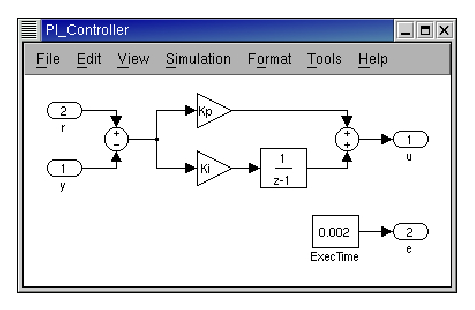
\includegraphics[scale=1]{block.ps}
\end{figure}

%%%%%%%%%%%%%%%%%%%%%%%%%%%%%%%%%%%%%%%%%%%%%%%%%%%

\entry{ttCreateCBS (I)}

\purpose
Create a soft or hard constant bandwidth server (CBS). 

\Msyntax
\begin{verbatim}
ttCreateCBS(name, Qs, Ts)
ttCreateCBS(name, Qs, Ts, type)
\end{verbatim}

\Csyntax
\begin{verbatim}
void ttCreateCBS(char *name, double Qs, double Ts)
void ttCreateCBS(char *name, double Qs, double Ts, int type)
\end{verbatim}

\args
\begin{tabularx}{\hsize}{l>{\raggedright\arraybackslash}X}
  {\tt name} & The name of the CBS. \\
  {\tt Qs} & The execution budget per server period. \\
  {\tt Ts} & The server period. \\
\end{tabularx}

\optargs
\begin{tabularx}{\hsize}{l>{\raggedright\arraybackslash}X}
  {\tt type} & The server type: 0 = Soft CBS (default), 1 = Hard CBS.
\end{tabularx}

\descr This function is used to create a constant bandwidth server
(CBS), to be used under EDF scheduling. Any number of tasks may be
attached to a CBS. The tasks in the CBS inherit the absolute deadline
of the CBS. If the tasks consume more than the execution budget in a
server period, the deadline of the CBS is postponed by one period. In
the case of Hard CBS, all tasks associated with the CBS are also put to
sleep until the next server period.

\seealso
{\tt ttAttachCBS, ttInitKernel}

\reference
Abeni, L. and Buttazzo, G. (1998): ``Integrating multimedia
applications in hard real-time systems.'' In {\em Proc. 19th IEEE Real-time Systems Symposium}.

%%%%%%%%%%%%%%%%%%%%%%%%%%%%%%%%%%%%%%%%%%%%%%%%%%%

\entry{ttCreateEvent  (I)}

\purpose
Create a \textsc{TrueTime} event (condition variable). 

\Msyntax
\begin{verbatim}
ttCreateEvent(eventname)
ttCreateEvent(eventname, monitorname)
\end{verbatim}

\Csyntax
\begin{verbatim}
void ttCreateEvent(char *eventname) 
void ttCreateEvent(char *eventname, char *monitorname) 
\end{verbatim}

\args
\begin{tabularx}{\hsize}{l>{\raggedright\arraybackslash}X}
  {\tt eventname} & Name of the event. Must be a unique, non-empty string. \\
  {\tt monitorname} & Name of an already created monitor to which the
  event is to be associated.
\end{tabularx}

\descr This function is used to create an event in the
\textsc{TrueTime} kernel. Events may be free, or
associated with a monitor.

\seealso 
{\tt ttWait}, {\tt ttNotify}, {\tt ttNotifyAll}

%%%%%%%%%%%%%%%%%%%%%%%%%%%%%%%%%%%%%%%%%%%%%%%%%%%

\entry{ttCreateHandler  (I)}

\purpose
Create an interrupt handler.

\Msyntax
\begin{verbatim}
ttCreateHandler(name, priority, codeFcn)
ttCreateHandler(name, priority, codeFcn, data)
\end{verbatim}

\Csyntax
\begin{verbatim}
void ttCreateHandler(char *name, double priority, 
                              double (*codeFcn)(int, void*))
void ttCreateHandler(char *name, double priority, 
                  double (*codeFcn)(int, void*), void* data)
\end{verbatim}

\args
\begin{tabularx}{\hsize}{l>{\raggedright\arraybackslash}X}
  {\tt name} & Name of the handler. Must be a unique, non-empty string. \\
  {\tt priority} & Priority of the handler. This should be a non-negative
  value, where a small number represents a high priority.\\
  {\tt codeFcn} & The code function of the handler, where
  \texttt{codeFcn} is a string (name of an m-file) in the
  Matlab case and a function pointer in the C++ case. \\
  {\tt data} & An arbitrary data structure representing the local
  memory of the handler.
\end{tabularx}

\descr This function is used to create a handler that will be executed
in response to interrupts. Interrupt handlers may be associated with
timers, network interfaces, external interrupt channels, or
attached to tasks as overrun handlers. A handler may be associated
with many interrupt sources.

\seealso 
{\tt ttCreateTimer}, {\tt ttCreatePeriodicTimer}, {\tt
  ttAttachTriggerHandler}, \\ {\tt ttAttachNetworkHandler}, {\tt
  ttAttachDLHandler}, {\tt ttAttachWCETHandler} 

%%%%%%%%%%%%%%%%%%%%%%%%%%%%%%%%%%%%%%%%%%%%%%%%%%%

\entry{ttCreateJob  (TH)}

\purpose
Create a job of a task.

\Msyntax
\begin{verbatim}
ttCreateJob(taskname)
ttCreateJob(taskname, time)
\end{verbatim}

\Csyntax
\begin{verbatim}
void ttCreateJob(char *taskname)
void ttCreateJob(char *taskname, double time)
\end{verbatim}

\args
\begin{tabularx}{\hsize}{l>{\raggedright\arraybackslash}X}
  {\tt taskname} & Name of a task. \\
  {\tt taskname} & The time at which the job should be created (default=now).\\
\end{tabularx}

\descr This function is used to create jobs of tasks. If
there already is a job active for the task, the job is queued and
served as soon as possible. {\tt ttCreateJob} is called to activate
aperiodic tasks, i.e., tasks created using {\tt ttCreateTask}.
A call to {\tt ttCreateJob} will trigger the arrival hook of the task.
If there are no active jobs the release hook will be called as well.
Otherwise, the release hook will be called when the job is later
activated from the job queue.

\seealso
{\tt ttCreateTask}, {\tt ttKillJob}

%%%%%%%%%%%%%%%%%%%%%%%%%%%%%%%%%%%%%%%%%%%%%%%%%%%

\entry{ttCreateLog  (I)}

\purpose
Create a user-defined or task-related log.

\Msyntax
\begin{verbatim}
ttCreateLog(logname, variable, size)
ttCreateLog(taskname, logtype, variable, size)
\end{verbatim}

\Csyntax
\begin{verbatim}
void ttCreateLog(char* logname, char* variable, int size)
void ttCreateLog(char* taskname, int logtype, char* variable, int size)
\end{verbatim}

\args
\begin{tabularx}{\hsize}{l>{\raggedright\arraybackslash}X}
  {\tt logname} & The name of the user-defined log. Values can later
           be written using ttLogStart, ttLogStop, ttLogNow, or ttLogValue. \\
  {\tt variable} & The name of the variable in Matlab workspace to
  which the log will be written after the simulation. \\
  {\tt size} & The maximum number of elements in the log. \\
  {\tt taskname} & Name of the task for which the log is created.
\\
  {\tt logtype} & The task log type (see below). \\
\end{tabularx}

\descr This function is used to create logs for individual tasks. Five
pre-defined log types exist to log response time, release latency,
start latency, execution time, and context switch instances. These are
obtained by setting the variable \texttt{logtype} to any of the
constants one to four, respectively. It is also possible to create
five additional log structures for each task (by specifying log type
number six). These user-controlled logs are written to from the code
functions using the primitives {\tt ttLogStart}, {\tt ttLogStop}, 
{\tt ttLogNow}, and {\tt ttLogValue}. After the simulation the logged
attributes can be found in Matlab workspace, having the name specified by
\texttt{variable}.

The task log types are

\begin{tabularx}{\hsize}{l>{\raggedright\arraybackslash}X}
 1 & Response time log \\
 2  & Release latency log (time between arrival
   and release of each job) \\
 3  & Start latency log (time between arrival
                    and start of execution for each job) \\
 4  & Execution time log
\end{tabularx}

\example Logging of response time and input-output latency
\begin{small}
\begin{verbatim}
% In initialization script

% Automatic log of response time (type 1) 
ttCreateLog('ctrl_task', 1, 'Responsetime', 100);

% User log for logging of I/O latency 
ttCreateLog('mylog', 'IOlatency', 100);


% Code function
function [exectime, data] = ctrl(seg, data)

switch seg,
  case 1,
    ttLogStart('mylog');     % Start I/O logging in user log
    y = ttAnalogIn(1);       % Input
    data.u = calculateOutput(y);
    exectime = 0.003;
  case 2,
    ttLogStop('mylog');      % Stop and write log entry in user log
    ttAnalogOut(1, data.u);  % Output
    exectime = -1;
end
\end{verbatim}
\end{small}

\seealso
{\tt ttLogNow}, {\tt ttLogStart}, {\tt ttLogStop}

%%%%%%%%%%%%%%%%%%%%%%%%%%%%%%%%%%%%%%%%%%%%%%%%%%%

\entry{ttCreateMailbox  (I)}

\purpose
Create a \textsc{TrueTime} mailbox for inter-task communication.

\Msyntax
\begin{verbatim}
ttCreateMailbox(mailboxname)
ttCreateMailbox(mailboxname, maxsize)
\end{verbatim}

\Csyntax
\begin{verbatim}
void ttCreateMailbox(char *mailboxname) 
void ttCreateMailbox(char *mailboxname, int maxsize) 
\end{verbatim}

\args
\begin{tabularx}{\hsize}{l>{\raggedright\arraybackslash}X}
  {\tt mailboxname} & Name of the mailbox. Must be a unique, non-empty
  string. \\
  {\tt maxsize} & The size of the buffer associated with the mailbox
  (default is INT\_MAX)
\end{tabularx}

\descr This function is used to create a mailbox for communication
between tasks. The \textsc{TrueTime} mailbox implements asynchronous
message passing with indirect naming. A buffer is used to store
incoming messages, and the maximum size of this buffer may be
specified by {\tt maxsize}.

\seealso 
{\tt ttTryPost}, {\tt ttTryFetch}, {\tt ttPost}, {\tt ttFetch}, {\tt ttRetrieve}

%%%%%%%%%%%%%%%%%%%%%%%%%%%%%%%%%%%%%%%%%%%%%%%%%%%

\entry{ttCreateMonitor  (I)}

\purpose
Create a \textsc{TrueTime} monitor.

\Msyntax
\begin{verbatim}
ttCreateMonitor(name, display)
\end{verbatim}

\Csyntax
\begin{verbatim}
void ttCreateMonitor(char *name, bool display)
\end{verbatim}

\args
\begin{tabularx}{\hsize}{l>{\raggedright\arraybackslash}X}
  {\tt name} & Name of the monitor. Must be a unique, non-empty string. \\
  {\tt display} & To indicate if the monitor should be included in the
  monitor graph generated by the simulation.
\end{tabularx}

\descr This function is used to create a monitor for task
synchronization. Condition variables for the monitor can be created
using {\tt ttCreateEvent}. The kernel block has a monitor output that
will display a graph showing when the various tasks have access to the
monitors.

\seealso 
{\tt ttEnterMonitor}, {\tt ttExitMonitor}, {\tt ttCreateEvent},
{\tt ttWait}, {\tt ttNotify}, {\tt ttNotifyAll}

%%%%%%%%%%%%%%%%%%%%%%%%%%%%%%%%%%%%%%%%%%%%%%%%%%%

\entry{ttCreatePeriodicTask  (I)}

\purpose
Create a periodic \textsc{TrueTime} task.

\Msyntax
\begin{verbatim}
ttCreatePeriodicTask(name, starttime, period, codeFcn)
ttCreatePeriodicTask(name, starttime, period, codeFcn, data)
\end{verbatim}

\Csyntax
\begin{verbatim}
void ttCreatePeriodicTask(char* name, double starttime, double period,
       double (*codeFcn)(int, void*))
void ttCreatePeriodicTask(char* name, double starttime, double period,
       double (*codeFcn)(int, void*), void* data)
\end{verbatim}

\args
\begin{tabularx}{\hsize}{l>{\raggedright\arraybackslash}X}
  {\tt name} & Name of the task. Must be a unique, non-empty string. \\
  {\tt starttime} & Release time for the first job of the periodic
  task.\\
  {\tt period} & Period of the task. \\
  {\tt codeFcn} & The code function of the task, where
  \texttt{codeFcn} is a string (name of an m-file) in the
  Matlab case and a function pointer in the C++ case. \\
  {\tt data} & An arbitrary data structure representing the local
  memory of the task.
\end{tabularx}

\descr This function is used to create a periodic task to run in the
\textsc{TrueTime} kernel. The periodicity is implemented internally by
the kernel using a periodic timer. See the simple PID-control example
in \texttt{\$DIR/examples/simple} for other ways to implement
periodic activities. {\it The deadline and worst-case execution time
  of the task are by default set equal to the task period}. This may
be changed by a suitable set-function.

\seealso 
{\tt ttCreateTask}, {\tt ttSetX}

%%%%%%%%%%%%%%%%%%%%%%%%%%%%%%%%%%%%%%%%%%%%%%%%%%%

\entry{ttCreatePeriodicTimer  (ITH)}

\purpose
Create a periodic timer and associate an interrupt handler with the timer.

\Msyntax
\begin{verbatim}
ttCreatePeriodicTimer(timername, period, handlername)
ttCreatePeriodicTimer(timername, offset, period, handlername)
\end{verbatim}

\Csyntax
\begin{verbatim}
void ttCreatePeriodicTimer(char *timername, double period, char *handlername)
void ttCreatePeriodicTimer(char *timername, double offset, double period, 
                           char *handlername)
\end{verbatim}

\args
\begin{tabularx}{\hsize}{l>{\raggedright\arraybackslash}X}
  {\tt timername} & Name of the timer. Must be unique, non-empty
  string.\\
  {\tt offset} & The time for the first expiry of the timer (default =
  0). \\
  {\tt period} & The period of the timer. \\
  {\tt handlername} & Name of interrupt handler associated with the timer.
\end{tabularx}

\descr This function is used to create a periodic timer. Each time the
timer expires the associated interrupt handler is activated and
scheduled for execution.

\seealso
{\tt ttCreateInterruptHandler}, {\tt ttCreateTimer}, {\tt ttRemoveTimer}

%%%%%%%%%%%%%%%%%%%%%%%%%%%%%%%%%%%%%%%%%%%%%%%%%%%

\entry{ttCreateSemaphore  (I)}

\purpose
Create a simple, counting \textsc{TrueTime} semaphore.

\Msyntax
\begin{verbatim}
ttCreateSemaphore(name, initval)
ttCreateSemaphore(name, initval, maxval)
\end{verbatim}

\Csyntax
\begin{verbatim}
void ttCreateSemaphore(char *name, int initval)
void ttCreateSemaphore(char *name, int initval, int maxval)
\end{verbatim}

\args
\begin{tabularx}{\hsize}{l>{\raggedright\arraybackslash}X}
  {\tt name} & Name of the semaphore. Must be a unique, non-empty string. \\
  {\tt initval} & The initial value of the semaphore. Must be an integer. \\
  {\tt maxval} & The maximum value of the semaphore.  Must be an
  integer. The default
  maximum value is INT\_MAX.
\end{tabularx}

\descr This function is used to create a simple, counting semaphore.
Semaphores can be used to synchronize tasks, for instance, to
synchronize a producer and a consumer task. Note that a semaphore does
not have the concept of a current owner task and hence should not be
used to achieve mutual exclusion.

The {\tt ttGive} command has no effect if the current value of the
semaphore is equal to {\tt maxval}. To create a binary
semaphore, set {\tt maxval} to 1.

Compared to \textsc{TrueTime} monitors, \textsc{TrueTime} sempahores
do not produce any output graphs. Also, they do not support any
priority inheritance protocol, but rather implement a simple FIFO
waiting queue. 

\seealso 
{\tt ttTake}, {\tt ttGive}

%%%%%%%%%%%%%%%%%%%%%%%%%%%%%%%%%%%%%%%%%%%%%%%%%%%

\entry{ttCreateTask  (I)}

\purpose
Create an aperiodic \textsc{TrueTime} task.

\Msyntax
\begin{verbatim}
ttCreateTask(name, deadline, codeFcn)
ttCreateTask(name, deadline, codeFcn, data)
\end{verbatim}

\Csyntax
\begin{verbatim}
void ttCreateTask(char* name, double deadline,
                  double (*codeFcn)(int, void*))
void ttCreateTask(char *name, double deadline,
                  double (*codeFcn)(int, void*), void* data)  
\end{verbatim}

\args
\begin{tabularx}{\hsize}{l>{\raggedright\arraybackslash}X}
  {\tt name} & Name of the task. Must be a unique, non-empty string. \\
  {\tt deadline} & Relative deadline of the task. \\
  {\tt codeFcn} & The code function of the task, where
  \texttt{codeFcn} is a string (name of an m-file) in the
  Matlab case and a function pointer in the C++ case. \\
  {\tt data} & An arbitrary data structure representing the local
  memory of the task.
\end{tabularx}

\descr This function is used to create a task to run in the
\textsc{TrueTime} kernel. 
{\it The worst-case execution time of the task is by default set equal
  to the task deadline}. This may be changed by a suitable
set-function.

\seealso 
{\tt ttCreatePeriodicTask}, {\tt ttCreateJob}, {\tt ttSetX}

%%%%%%%%%%%%%%%%%%%%%%%%%%%%%%%%%%%%%%%%%%%%%%%%%%%

\entry{ttCreateTBS  (I)}

\purpose
Create a total bandwidth server (TBS).

%%%%%%%%%%%%%%%%%%%%%%%%%%%%%%%%%%%%%%%%%%%%%%%%%%%

\entry{ttCreateTimer  (ITH)}

\purpose
Create a one-shot timer and associate an interrupt handler with the timer.

\Msyntax
\begin{verbatim}
ttCreateTimer(timername, time, handlername)
\end{verbatim}

\Csyntax
\begin{verbatim}
void ttCreateTimer(char *timername, double time, char *handlername)
\end{verbatim}

\args
\begin{tabularx}{\hsize}{l>{\raggedright\arraybackslash}X}
    {\tt timername} & Name of the timer. Must be unique, non-empty
  string.\\
  {\tt time} & The time when the timer is set to expire. \\
  {\tt handlername} & Name of interrupt handler associated with the timer.
\end{tabularx}

\descr This function is used to create a one-shot timer. When the
timer expires the associated interrupt handler is activated and
scheduled for execution. 

\seealso
{\tt ttCreateInterruptHandler}, {\tt ttCreatePeriodicTimer}, {\tt ttRemoveTimer}

%%%%%%%%%%%%%%%%%%%%%%%%%%%%%%%%%%%%%%%%%%%%%%%%%%%

\entry{ttCreateTimeTriggeredDispatcher  (I)}

\purpose
Create a time-triggered dispatcher.

%%%%%%%%%%%%%%%%%%%%%%%%%%%%%%%%%%%%%%%%%%%%%%%%%%%

\entry{ttCurrentTask  (TH)}

\purpose
Get the name of the currently executing task (user task or handler).

%%%%%%%%%%%%%%%%%%%%%%%%%%%%%%%%%%%%%%%%%%%%%%%%%%%

\entry{ttCurrentTime  (ITH)}

\purpose
Get and/or set the current time in the simulation on a per node basis.

\Msyntax
\begin{verbatim}
time = ttCurrentTime
time = ttCurrentTime(newTime)
\end{verbatim}

\Csyntax
\begin{verbatim}
double ttCurrentTime()
double ttCurrentTime(double newTime)
\end{verbatim}

\args
\begin{tabularx}{\hsize}{l>{\raggedright\arraybackslash}X}
  {\tt newTime} & Sets the current time to this time. \\
\end{tabularx}

\descr This function returns the current time in the simulation, in
seconds. When the function is used to set the current time, the old
current time is returned.

%%%%%%%%%%%%%%%%%%%%%%%%%%%%%%%%%%%%%%%%%%%%%%%%%%%

\entry{ttDiscardUnsentMessages (IT)}

\purpose
Delete unsent messages in the network queue.

\Msyntax
\begin{verbatim}
nbr = ttDiscardUnsentMessages
nbr = ttDiscardUnsentMessages(network)
\end{verbatim}

\Csyntax
\begin{verbatim}
int ttDiscardUnsentMessages()
int ttDiscardUnsentMessages(int network)
\end{verbatim}

\args
\begin{tabularx}{\hsize}{l>{\raggedright\arraybackslash}X}
  {\tt network} & The network interface from which  messages should be
              deleted (default is 1). \\
\end{tabularx}

\descr This function can be used to delete any unsent messages waiting
in the network interface output queue. A message that has already
started to be sent is not affected. The function returns the total
number of deleted messages.

%%%%%%%%%%%%%%%%%%%%%%%%%%%%%%%%%%%%%%%%%%%%%%%%%%%

\entry{ttEnableSlotShifting  (I)}

\purpose
Enable slot shifting.

%%%%%%%%%%%%%%%%%%%%%%%%%%%%%%%%%%%%%%%%%%%%%%%%%%%

\entry{ttEnterMonitor  (T)}

\purpose
Enter a monitor, blocking if the monitor is not free.

\Msyntax
\begin{verbatim}
ttEnterMonitor(monitorname) 
\end{verbatim}

\Csyntax
\begin{verbatim}
void ttEnterMonitor(char *monitorname) 
\end{verbatim}

\args
\begin{tabularx}{\hsize}{l>{\raggedright\arraybackslash}X}
  {\tt monitorname} & Name of a monitor.
\end{tabularx}

\descr This function is used to attempt to enter a monitor. If the
attempt fails, the task will be removed from the ready queue and
inserted in the waiting queue of the monitor (the waiting queue is
sorted using the priority function in the same way as the ready
queue). This will also trigger the suspend hook of the task.

When the task currently holding the monitor exits, the first task in
the waiting queue will be moved to the ready queue and is now holding
the monitor. Execution will then resume in the segment after the call
to \texttt{ttEnterMonitor}. To ensure that no further instructions are
executed in the case that \texttt{ttEnterMonitor} fails, it needs to
be called from its own segment (since all code of a \textsc{TrueTime}
segment is executed at once before scheduling decisions are made). See
the example below.

To avoid \textit{priority inversion}, standard \textit{priority
  inheritance} is used if a task tries to enter a monitor currently
held by a lower priority task.

\example 

\begin{footnotesize}
\begin{verbatim}
function [exectime, data] = ctrl(seg, data)
switch seg,
  case 1, 
    ttEnterMonitor('mutex');
    exectime = 0;
  case 2,
    if some_condition_not_fulfilled
      ttWait('condvar');
      ttSetNextSegment(2);
      exectime = 0;
    else
      criticalOperation;
      exectime = 0.005;
    end
  case 3,
    ttExitMonitor('mutex');
    exectime = -1;
end
\end{verbatim}
\end{footnotesize}

\seealso
{\tt ttCreateMonitor}, {\tt ttExitMonitor}, {\tt ttCreateEvent}, {\tt
  ttWait}, {\tt ttNotify}, {\tt ttNotifyAll}

%%%%%%%%%%%%%%%%%%%%%%%%%%%%%%%%%%%%%%%%%%%%%%%%%%%

\entry{ttExitMonitor  (T)}

\purpose
Exit a monitor.

\Msyntax
\begin{verbatim}
ttExitMonitor(monitorname) 
\end{verbatim}

\Csyntax
\begin{verbatim}
void ttExitMonitor(char *monitorname) 
\end{verbatim}

\args
\begin{tabularx}{\hsize}{l>{\raggedright\arraybackslash}X}
  {\tt monitorname} & Name of a monitor.
\end{tabularx}

\descr This function is used to exit a monitor. The function can only
be called by the task currently holding the monitor. The call will
cause the first task in the waiting queue of the monitor to be moved
to the ready queue. To ensure that no further instructions are
executed in the case that a context switch should occur when the
monitor is released, \texttt{ttExitMonitor} needs to
be called from its own segment (since all code of a \textsc{TrueTime}
segment is executed at once before scheduling decisions are made). 

\example See \texttt{ttEnterMonitor}.

\seealso
{\tt ttCreateMonitor}, {\tt ttEnterMonitor}

%%%%%%%%%%%%%%%%%%%%%%%%%%%%%%%%%%%%%%%%%%%%%%%%%%%

\entry{ttFetch  (T)}

\purpose
Fetch a message from a mailbox, blocking if the mailbox is empty.

\Msyntax
\begin{verbatim}
ttFetch(mailboxname) 
\end{verbatim}

\Csyntax
\begin{verbatim}
void ttFetch(char *mailboxname) 
\end{verbatim}

\args
\begin{tabularx}{\hsize}{l>{\raggedright\arraybackslash}X}
  {\tt mailboxname} & Name of a mailbox.
\end{tabularx}

\descr This function is used to wait for a message at a mailbox. If
the mailbox is empty, the task will be blocked until a message has
arrived. Tasks waiting to fetch from a mailbox are sorted in FIFO order. 

Note that this function does not read the actual message -- that is
done using {\tt ttRetrieve}. (This somewhat akward solution is due to
the segment structure of \textsc{TrueTime}.) 

\example 
\begin{small}
\begin{verbatim}
function [exectime, data] = ctrl(seg, data)
switch seg,
  case 1, 
    ttFetch('mailbox');            % wait for a message
    exectime = 0;
  case 2,
    msg = ttRetrieve('mailbox');   % read the actual message
    doStuff;
    exectime = 0.005;
  case 3,
    exectime = -1;
end
\end{verbatim}
\end{small}

\seealso
{\tt ttCreateMailbox}, {\tt ttTryPost}, {\tt ttTryFetch}, {\tt ttPost},
{\tt ttRetrieve}

%%%%%%%%%%%%%%%%%%%%%%%%%%%%%%%%%%%%%%%%%%%%%%%%%%%

\entry{ttGetData  (TH)}

\purpose
Retrieve the local memory data structure associated with a specific task.

\Msyntax
\begin{verbatim}
data = ttGetData(taskname)
\end{verbatim}

\Csyntax
\begin{verbatim}
void *ttGetData(char *taskname)
\end{verbatim}


\args
\begin{tabularx}{\hsize}{l>{\raggedright\arraybackslash}X}
  {\tt taskname} & Name of a task. \\
\end{tabularx}

\descr This function is used to retrieve the data structure of a
specific task. The data structure represents local memory of the task
and is normally updated in the code function of the task. Using this
function in combination with \texttt{ttSetData} it is possible to
modify the data also outside the code function.

\seealso
\texttt{ttSetData, ttCreateTask, ttCreatePeriodicTask}

%%%%%%%%%%%%%%%%%%%%%%%%%%%%%%%%%%%%%%%%%%%%%%%%%%%

\entry{ttGetInitArg (C++ only) (I)}

\purpose
Retrieve a pointer to the init argument of the \textsc{TrueTime} block.

\Csyntax
\begin{verbatim}
mxArray *ttGetInitArg()
\end{verbatim}

%%%%%%%%%%%%%%%%%%%%%%%%%%%%%%%%%%%%%%%%%%%%%%%%%%%

\entry{ttGetInvoker (H)}

\purpose
Get the name of the interrupt source that invoked a handler.

\Msyntax
\begin{verbatim}
invoker = ttGetInvoker
\end{verbatim}

\Csyntax
\begin{verbatim}
char *ttGetInvoker()
\end{verbatim}

\descr This function returns the name of the external trigger, network
interface, or overrun timer that triggered running handler.

%%%%%%%%%%%%%%%%%%%%%%%%%%%%%%%%%%%%%%%%%%%%%%%%%%%

\entry{ttGetMsg  (TH)}

\purpose
Get a message that has been received over a network. This function is
used both for wired and wireless networks.

\Msyntax
\begin{verbatim}
[msg, signalPower] = ttGetMsg
[msg, signalPower] = ttGetMsg(network)
\end{verbatim}


\Csyntax
\begin{verbatim}
void *ttGetMsg()
void *ttGetMsg(int network)
void *ttGetMsg(int network, double *signalPower)
\end{verbatim}


\args
\begin{tabularx}{\hsize}{l>{\raggedright\arraybackslash}X}
  {\tt network} & The network interface from which the message should be
  received. Can be omitted if the kernel is only connected to one network. \\
  {\tt signalPower} & The value of the received signal power
  corresponding to this message. Only used in the wireless network.\\
\end{tabularx}

\descr This function is used to retrieve a message that has been
received over the network. Typically, you have been notified that a
message exists in the network interface input queue by an interrupt,
but it is also possible to poll for new messages. If no message
exists, the function will return NULL (C++) or an empty matrix
(Matlab). 

\example
\begin{small}
\begin{verbatim}
% Task that waits for and reads messages 
function [exectime, data] = receiver(seg, data)
switch seg,
  case 1, 
    ttWait('message');
    exectime = 0;
  case 2,
    msg = ttGetMsg;
    disp('I got a message!');
    exectime = 0.001;
  case 3,
    ttSetNextSegment(1); % loop back and wait for new message
    exectime = 0;
end
% Interrupt handler that is called by the network interface 
function [exectime, data] = msgRcvhandler(seg, data)
ttNotifyAll('message');
exectime = -1;
\end{verbatim}
\end{small}

\enlargethispage{\baselineskip}
\seealso
\texttt{ttAttachNetworkHandler, ttSendMsg}

%%%%%%%%%%%%%%%%%%%%%%%%%%%%%%%%%%%%%%%%%%%%%%%%%%%

\entry{ttGetX  (ITH)}

\purpose
Get a specific task attribute.

\Msyntax
\begin{verbatim}
value = ttGetX
value = ttGetX(taskname)
\end{verbatim}

\Csyntax
\begin{verbatim}
double ttGetX()
double ttGetX(char *taskname)
\end{verbatim}

\args
\begin{tabularx}{\hsize}{l>{\raggedright\arraybackslash}X}
  {\tt taskname} & Name of a task. 
\end{tabularx}

\descr These functions are used to retrieve values of task attributes. There
exist functions for the following attributes (with the true function name
in parenthesis):
\begin{itemize}
  \item arrival time (\texttt{ttGetArrival})
  \item release time (\texttt{ttGetRelease})
  \item relative deadline (\texttt{ttGetDeadline})
  \item absolute deadline (\texttt{ttGetAbsDeadline})
  \item priority (\texttt{ttGetPriority})
  \item period (\texttt{ttGetPeriod})
  \item worst-case execution time (\texttt{ttGetWCET})
  \item execution time budget (\texttt{ttGetBudget})
\end{itemize}

Use the \texttt{ttGetX} functions to retrieve the current attributes
of a task. All the functions exist in overloaded versions as shown by
the syntax above. If the argument \texttt{taskname} is not specified,
the call will affect the currently running task. Below follow some
special notes on the individual functions:

{\it ttGetArrival:} Returns the time when the current task job
was created. An error will occur if the task has no running job.

{\it ttGetRelease:} Returns the time when the current task job
was released. An error will occur if the task has no running job.

{\it ttGetDeadline:} Returns the relative deadline of the task.

{\it ttGetAbsDeadline:} Returns the absolute deadline of the current
task job. An error will occur if the task has no running job.

{\it ttGetPriority:} Returns the assigned base priority of the task. 

{\it ttGetPeriod:} Returns the period of a periodic task. An error
will occur if the task is not periodic.

{\it ttGetWCET:} Returns the worst-case execution time of a task. 

{\it ttGetBudget:} Returns the remaining execution time budget of the
current task job. The execution time budget is decreased each
time a new segment of the code function is executed, as well as when
the task is suspended by another task. The execution time budget is
reset to the worst-case execution time at the start of each task job.

\seealso
\texttt{ttSetX} 

%%%%%%%%%%%%%%%%%%%%%%%%%%%%%%%%%%%%%%%%%%%%%%%%%%%

\entry{ttGive (TH)}

\purpose
Give (signal) a semaphore.

\Msyntax
\begin{verbatim}
ttGive(semname)
\end{verbatim}

\Csyntax
\begin{verbatim}
void ttGive(char *semname)
\end{verbatim}

\args
\begin{tabularx}{\hsize}{l>{\raggedright\arraybackslash}X}
  {\tt semname} & The name of the semaphore.\\
\end{tabularx}

\descr This function is used to signal a semaphore. Its semantics can
be described by the following pseudo-code:
\begin{verbatim}
if (value < maxval) {
  value++;
  if (value <= 0) {
    release the first task from the semaphore queue;
  }
}
\end{verbatim}

\seealso
{\tt ttCreateSemaphore}, {\tt ttTake}

%%%%%%%%%%%%%%%%%%%%%%%%%%%%%%%%%%%%%%%%%%%%%%%%%%%

\entry{ttInitKernel (I)}

\purpose
Initialize the \textsc{TrueTime} kernel.

\Msyntax
\begin{verbatim}
ttInitKernel(prioFcn)
ttInitKernel(prioFcn, contextSwitchOverhead)
\end{verbatim}

\Csyntax
\begin{verbatim}
void ttInitKernel(double (*prioFcn)(UserTask*))
void ttInitKernel(double (*prioFcn)(UserTask*), double contextSwitchOverhead)
\end{verbatim}

\args
\begin{tabularx}{\hsize}{l>{\raggedright\arraybackslash}X}
  {\tt prioFcn} & The scheduling policy used by the kernel. \\
  {\tt contextSwitchOverhead} & The overhead time for a context switch. Optional
  argument, taken as zero if not specified.
\end{tabularx}

\descr This function performs necessary initializations of the
kernel block and \emph{must} be called first of all in the
initialization script. The priority function should be one of the
following in the Matlab case: \texttt{'prioFP'} (fixed-priority
scheduling), \texttt{'prioDM'} (deadline-monotonic scheduling), or
\texttt{'prioEDF'} (earliest-deadline-first scheduling, with support
for constant/total bandwidth servers). A task associated with a CBS/TBS is
scheduled according to the deadline of the CBS/TBS and not of the task.

In the C++ case, an arbitrary priority function can be supplied. There
are predefined priority functions called \texttt{prioFP},
\texttt{prioDM}, and \texttt{prioEDF}.

The schedule plot for the context switches can be turned off by a call
to \texttt{ttNoSchedule('CShandler')}.

\example The pre-defined priority functions
for deadline-monotonic scheduling and earliest-deadline-first
scheduling are given below. Note that a small return value corresponds
to a high priority.

\begin{footnotesize}
\begin{verbatim}
/* Priority function for deadline-monotonic scheduling */
double prioDM(UserTask* t) {
  return t->deadline;
}

/* Priority function for earliest-deadline-first scheduling,
   with support for constant bandwidth servers */
double prioEDF(UserTask* t) {
  if (t->cbs) {
    // The task is associated with a CBS: inherit the deadline of the CBS
    return t->cbs->ds;
  } else {
    // No CBS: return the absolute deadline of the task
    return t->absDeadline;
  }
}
\end{verbatim}
\end{footnotesize}

%%%%%%%%%%%%%%%%%%%%%%%%%%%%%%%%%%%%%%%%%%%%%%%%%%%

\entry{ttKillJob  (TH)}

\purpose
Kill the current job of a task.

\Msyntax
\begin{verbatim}
ttKillJob(taskname)
\end{verbatim}

\Csyntax
\begin{verbatim}
void ttKillJob(char *taskname)
\end{verbatim}

\args
\begin{tabularx}{\hsize}{l>{\raggedright\arraybackslash}X}
  {\tt taskname} & Name of a task. \\
\end{tabularx}

\descr This function is used to kill the current active job of a task.
The finish hook of the task will be called as the job is killed. If
there exist pending jobs for the task that should be released, the
first job in the queue will be scheduled for execution and the release
hook will be called.

\seealso
{\tt ttCreateJob}

%%%%%%%%%%%%%%%%%%%%%%%%%%%%%%%%%%%%%%%%%%%%%%%%%%%

\entry{ttLogNow  (TH)}

\purpose
Log the current time in a user-defined log.

\Msyntax
\begin{verbatim}
ttLogNow(logname)
\end{verbatim}

\Csyntax
\begin{verbatim}
void ttLogNow(char *logname) 
\end{verbatim}

\args
\begin{tabularx}{\hsize}{l>{\raggedright\arraybackslash}X}
  {\tt logname} & The name of the user-defined log. \\
\end{tabularx}

\descr This function is used to write the current time in a user-defined
log.

\seealso
{\tt ttCreateLog}, {\tt ttLogStart}, {\tt ttLogStop}, {\tt ttLogValue}   

%%%%%%%%%%%%%%%%%%%%%%%%%%%%%%%%%%%%%%%%%%%%%%%%%%%

\entry{ttLogStart  (TH)}

\purpose
Start a timing measurement in a user-defined log.

\Msyntax
\begin{verbatim}
ttLogStart(logname)
\end{verbatim}

\Csyntax
\begin{verbatim}
void ttLogStart(int logname)
\end{verbatim}

\args
\begin{tabularx}{\hsize}{l>{\raggedright\arraybackslash}X}
  {\tt logID} & The name of the user-defined log. \\
\end{tabularx}

\descr This function is used to start a timing measurement in a user-defined
log. Nothing is written in the log until a subsequent call to
\texttt{ttLogStop}.

\example See the example in the description of \texttt{ttCreateLog}
that shows how to use \texttt{ttLog\-Start} and \texttt{ttLogStop} to
log input-output latency in a code function.

\seealso
{\tt ttCreateLog}, {\tt ttLogStop}, {\tt ttLogNow}, {\tt ttLogValue} 

%%%%%%%%%%%%%%%%%%%%%%%%%%%%%%%%%%%%%%%%%%%%%%%%%%%

\entry{ttLogStop  (TH)}

\purpose
Stop a timing measurement in a user-defined log.

\Msyntax
\begin{verbatim}
ttLogStop(logname)
\end{verbatim}

\Csyntax
\begin{verbatim}
void ttLogStop(int logname) 
\end{verbatim}

\args
\begin{tabularx}{\hsize}{l>{\raggedright\arraybackslash}X}
  {\tt logname} & The name of the user-defined log. \\
\end{tabularx}

\descr This function is used to stop a timing measurement in a user-defined
log. When this function is called, the difference between the current time and
the time of the associated \texttt{ttLogStart} will be written in the log.

\example See the example in the description of \texttt{ttCreateLog}
that shows how to use \texttt{ttLog\-Start} and \texttt{ttLogStop} to
log input-output latency in a code function.

\seealso
{\tt ttCreateLog}, {\tt ttLogStart}, {\tt ttLogNow}, {\tt ttLogValue} 

%%%%%%%%%%%%%%%%%%%%%%%%%%%%%%%%%%%%%%%%%%%%%%%%%%%

\entry{ttLogValue  (TH)}

\purpose
Log a scalar value in a user-defined log.

\Msyntax
\begin{verbatim}
ttLogValue(logname, value)
\end{verbatim}

\Csyntax
\begin{verbatim}
void ttLogValue(char *logname, double value) 
\end{verbatim}

\args
\begin{tabularx}{\hsize}{l>{\raggedright\arraybackslash}X}
  {\tt logname} & The name of the user-defined log. \\
  {\tt value} & The scalar value to log. \\
\end{tabularx}

\descr This function is used to write the current time in a user-defined log.

\seealso
{\tt ttCreateLog}, {\tt ttLogStart}, {\tt ttLogStop}, {\tt ttLogNow} 

%%%%%%%%%%%%%%%%%%%%%%%%%%%%%%%%%%%%%%%%%%%%%%%%%%%

\entry{ttNonPreemptible  (I)}

\purpose
Make a user task or handler non-preemptible.

\Msyntax
\begin{verbatim}
ttNonPreemptible(taskname)
\end{verbatim}

\Csyntax
\begin{verbatim}
void ttNonPreemptible(char* taskname)
\end{verbatim}

\args
\begin{tabularx}{\hsize}{l>{\raggedright\arraybackslash}X}
  {\tt taskname} & Name of a task. \\
\end{tabularx}

\descr Tasks are by default preemptible. Use this function to specify
that a task can not be preempted by other tasks. Non-preemptible tasks
may, however, still be preempted by interrupts.

%%%%%%%%%%%%%%%%%%%%%%%%%%%%%%%%%%%%%%%%%%%%%%%%%%%

\entry{ttNoSchedule  (I)}

\purpose
Switch off the schedule plot for a specific task or interrupt
handler. 

\Msyntax
\begin{verbatim}
ttNoSchedule(name)
\end{verbatim}

\Csyntax
\begin{verbatim}
void ttNoSchedule(char* name)
\end{verbatim}

\args
\begin{tabularx}{\hsize}{l>{\raggedright\arraybackslash}X}
  {\tt name} & Name of a task or interrupt handler. \\
\end{tabularx}

\descr This function is used to switch off the schedule plot for
a specific task or interrupt handler. The schedule output is generated by
default and this function must be called to turn it off. This function
can only be called from the initialization script.

The schedule plot for the context switches can be turned off by
specifying the name \texttt{'CShandler'}.

%%%%%%%%%%%%%%%%%%%%%%%%%%%%%%%%%%%%%%%%%%%%%%%%%%%

\entry{ttNotify  (TH)}

\purpose
Notify the highest-priority task waiting for an event.

\Msyntax
\begin{verbatim}
ttNotify(eventname) 
\end{verbatim}

\Csyntax
\begin{verbatim}
void ttNotify(char *eventname) 
\end{verbatim}

\args
\begin{tabularx}{\hsize}{l>{\raggedright\arraybackslash}X}
  {\tt eventname} & Name of an event.
\end{tabularx}

\descr This function is used to notify the first task in the waiting
queue associated with an event. The waiting queue is sorted according
to the priority function of the kernel (in the same way as the ready
queue). If the event is associated with a monitor, {\tt ttNotify} must
be performed inside a \texttt{ttEnterMonitor-ttExitMo\-nitor}
construct. The highest-priority waiting task will be moved to the
waiting queue of the associated monitor, or directly to the ready
queue if it is a free event.

\seealso
{\tt ttCreateEvent}, {\tt ttWait}, {\tt ttNotifyAll}

%%%%%%%%%%%%%%%%%%%%%%%%%%%%%%%%%%%%%%%%%%%%%%%%%%%

\entry{ttNotifyAll  (TH)}

\purpose
Notify all tasks waiting for an event.

\Msyntax
\begin{verbatim}
ttNotifyAll(eventname) 
\end{verbatim}

\Csyntax
\begin{verbatim}
void ttNotifyAll(char *eventname) 
\end{verbatim}

\args
\begin{tabularx}{\hsize}{l>{\raggedright\arraybackslash}X}
  {\tt eventname} & Name of an event.
\end{tabularx}

\descr This function is used to notify all tasks waiting for an event.
If the event is associated with a monitor, {\tt ttNotifyAll} must be
performed inside a \texttt{ttEnterMonitor\-ttExitMonitor} construct.
The call will cause all tasks waiting for the event to be moved to the
waiting queue of the associated monitor, or directly to the ready
queue if it is a free event.

\seealso
{\tt ttCreateEvent}, {\tt ttWait}, {\tt ttNotify}

%%%%%%%%%%%%%%%%%%%%%%%%%%%%%%%%%%%%%%%%%%%%%%%%%%%

\entry{ttPost  (T)}

\purpose
Post a message to a mailbox, blocking if the mailbox is full.

\Msyntax
\begin{verbatim}
ttPost(mailboxname, msg) 
\end{verbatim}

\Csyntax
\begin{verbatim}
void ttPost(char *mailboxname, void* msg) 
\end{verbatim}

\args
\begin{tabularx}{\hsize}{l>{\raggedright\arraybackslash}X}
  {\tt mailboxname} & Name of a mailbox. \\
  {\tt msg} & An arbitrary data structure representing the contents of
  the message to be posted. \\
\end{tabularx}

\descr This function is used to post messages to a mailbox. If
the mailbox is full, the task will be blocked. Tasks waiting to post
to a mailbox are sorted in FIFO order.

\seealso
{\tt ttCreateMailbox}, {\tt ttTryPost}, {\tt ttTryFetch}, 
{\tt ttFetch}, {\tt ttRetrieve}


%%%%%%%%%%%%%%%%%%%%%%%%%%%%%%%%%%%%%%%%%%%%%%%%%%%

\entry{ttRemoveTimer  (TH)}

\purpose
Remove a specific timer.

\Msyntax
\begin{verbatim}
ttRemoveTimer(timername)
\end{verbatim}

\Csyntax
\begin{verbatim}
void ttRemoveTimer(char *timername)
\end{verbatim}

\args
\begin{tabularx}{\hsize}{l>{\raggedright\arraybackslash}X}
  {\tt timername} & Name of the timer to be removed. 
\end{tabularx}

\descr This function is used to remove timers. Both one-shot and
periodic timers can be removed by this function. Using this function
on a periodic timer will remove the timer completely, and not only the
current job.

\seealso
{\tt ttCreateTimer}, {\tt ttCreatePeriodicTimer}

%%%%%%%%%%%%%%%%%%%%%%%%%%%%%%%%%%%%%%%%%%%%%%%%%%%

\entry{ttRetrieve  (T)}

\purpose
Read a message that was fetched using {\tt ttFetch}.

\Msyntax
\begin{verbatim}
msg = ttRetrieve(mailboxname) 
\end{verbatim}

\Csyntax
\begin{verbatim}
void* ttRetrieve(char *mailboxname) 
\end{verbatim}

\args
\begin{tabularx}{\hsize}{l>{\raggedright\arraybackslash}X}
  {\tt mailboxname} & Name of a mailbox.
\end{tabularx}

\descr This function may only be called if {\tt ttFetch} was called in
the previous segment. It is used to read the fetched message. (This
somewhat akward solution is due to the fact that blocking primitives
in \textsc{TrueTime} cannot return any data.)

\example 
\begin{small}
\begin{verbatim}
function [exectime, data] = ctrl(seg, data)
switch seg,
  case 1, 
    ttFetch('mailbox');            % wait for a message
    exectime = 0;
  case 2,
    msg = ttRetrieve('mailbox');   % read the actual message
    doStuff;
    exectime = 0.005;
  case 3,
    exectime = -1;
end
\end{verbatim}
\end{small}

\seealso
{\tt ttTryPost}, {\tt ttTryFetch}, {\tt ttPost},
{\tt ttFetch}

%%%%%%%%%%%%%%%%%%%%%%%%%%%%%%%%%%%%%%%%%%%%%%%%%%%

\entry{ttSendMsg  (TH)}

\purpose
Send a message over a network.

\Msyntax
\begin{verbatim}
ttSendMsg(receiver, data, length)
ttSendMsg(receiver, data, length, priority)
ttSendMsg([network receiver], data, length)
ttSendMsg([network receiver], data, length, priority)
\end{verbatim}

\Csyntax
\begin{verbatim}
void ttSendMsg(int receiver, void *data, int length)
void ttSendMsg(int receiver, void *data, int length, int priority)
void ttSendMsg(int network, int receiver, void *data, int length)
void ttSendMsg(int network, int receiver, void *data, int length, int priority)
\end{verbatim}

\args
\begin{tabularx}{\hsize}{l>{\raggedright\arraybackslash}X}
  {\tt network} & The network interface on which the message should be
  sent. Can be omitted if the kernel is only connected to one network.  \\
  {\tt receiver} & The number of the receiving node (a number between
  1 and the number of nodes). It is allowed to send messages to
  oneself. Specify receiver number~0 to broadcast a message to all
  nodes in the network. \\
  {\tt data} & An arbitrary data structure representing the contents
  of the message. \\
  {\tt length} & The length of the message, in bits.
  Determines the time it will take to transmit the message.\\
  {\tt priority} & The priority of the message (relevant only for
  CSMA/AMP networks). If not specified, the priority will be
  given by the number of the sending node, i.e., messages sent from
  node 1 will have the highest priority by default.
\end{tabularx}

\seealso
\texttt{ttGetMsg}

%%%%%%%%%%%%%%%%%%%%%%%%%%%%%%%%%%%%%%%%%%%%%%%%%%%

\entry{ttSetCBSParameters  (ITH)}

\purpose
Change the parameters of a constant bandwidth server (CBS).

\Msyntax
\begin{verbatim}
ttSetCBSParameters(cbsname, Qs, Ts)
\end{verbatim}

\Csyntax
\begin{verbatim}
void ttSetCBSParameters(char *cbsname, double Qs, double Ts)
\end{verbatim}

\args
\begin{tabularx}{\hsize}{l>{\raggedright\arraybackslash}X}
  {\tt cbsname} & Name of a CBS. \\
  {\tt Qs} & Server budget. \\
  {\tt Ts} & Server period. \\
\end{tabularx}

\descr 

\seealso
\texttt{ttCreateCBS}

%%%%%%%%%%%%%%%%%%%%%%%%%%%%%%%%%%%%%%%%%%%%%%%%%%%

\entry{ttSetData  (TH)}

\purpose
Update the local memory data structure associated with a specific task.

\Msyntax
\begin{verbatim}
ttSetData(taskname, data)
\end{verbatim}

\args
\begin{tabularx}{\hsize}{l>{\raggedright\arraybackslash}X}
  {\tt taskname} & Name of a task. \\
  {\tt data} & Updated data structure. \\
\end{tabularx}

\descr This function is used to update the data structure of a
specific task. The data structure represents local memory of the task
and is normally updated in the code function of the task. Using this
function in combination with \texttt{ttGetData} it is possible to
modify the data also outside the code function.

The \texttt{ttSetData} function only exists in Matlab syntax. No C++
version is needed, since \texttt{ttGetData} gives a pointer to the
task data structure.

\seealso
\texttt{ttGetData, ttCreateTask, ttCreatePeriodicTask}

%%%%%%%%%%%%%%%%%%%%%%%%%%%%%%%%%%%%%%%%%%%%%%%%%%%

\entry{ttSetKernelParameter  (ITH)}

\purpose
Set a specific kernel parameter.

\Msyntax
\begin{verbatim}
ttSetKernelParameter(parameter, value)
\end{verbatim}

\Csyntax
\begin{verbatim}
void ttSetKernelParameter(char* parameter, double value)
\end{verbatim}

\args
\begin{tabularx}{\hsize}{l>{\raggedright\arraybackslash}X}
  {\tt parameter} & The name of the parameter to be changed.\\
  {\tt value} & The new value of the parameter. \\
\end{tabularx}

\descr This function makes it possible to change kernel parameters on
the fly. At the moment the following parameters are supported: 
\begin{itemize}
\item {\tt cpuscaling}
\item {\tt energyconsumption}
\end{itemize}
The default parameter value
is 1 for {\tt cpuscaling}, and 0 for {\tt energyconsumption}. Setting the
cpuscaling to 2 will make the kernel block execute everything twice as
fast as with 1. This makes it possible to experiment with different Dynamic
Voltage Scaling methods. At the same time the energy consumption can
be set to a realistic value and connected to a battery block.

%%%%%%%%%%%%%%%%%%%%%%%%%%%%%%%%%%%%%%%%%%%%%%%%%%%

\entry{ttSetNetworkParameter  (ITH)}

\purpose
Set a specific network parameter on a per node basis.

\Msyntax
\begin{verbatim}
ttSetNetworkParameter(parameter, value)
ttSetNetworkParameter(networkNbr, parameter, value)
\end{verbatim}

\Csyntax
\begin{verbatim}
void ttSetNetworkParameter(char* parameter, double value)
void ttSetNetworkParameter(int networkNbr, char* parameter, double value)
\end{verbatim}

\args
\begin{tabularx}{\hsize}{l>{\raggedright\arraybackslash}X}
  {\tt parameter} & The name of the parameter to be changed.\\
  {\tt value} & The new value of the parameter. \\
  {\tt networkNbr} & The network interface on which the parameter should
  be changed. Can be omitted if the kernel is only connected to one network. \\
\end{tabularx}

\descr This function makes it possible to change network parameters on
a per node basis. At the moment the following parameters are
supported: 
\begin{description}
\item[\tt 'transmitpower'] The transmitpower parameter is only valid when using the
wireless network and defaults to whatever is set in the block mask.
\item[\tt 'predelay'] The time a message is
delayed by the network interface on the sending end. This can be used
to model, e.g., a slow serial connection between the computer and the
network interface. The default value is zero.
\item[\tt 'postdelay'] The time a message is
delayed by the network interface on the receiving end.  The default
value is zero. 
\end{description}


%%%%%%%%%%%%%%%%%%%%%%%%%%%%%%%%%%%%%%%%%%%%%%%%%%%

\entry{ttSetNextSegment  (TH)}

\purpose
Set the next segment to be executed in the code function.

\Msyntax
\begin{verbatim}
ttSetNextSegment(segment)
\end{verbatim}

\Csyntax
\begin{verbatim}
void ttSetNextSegment(int segment)
\end{verbatim}

\args
\begin{tabularx}{\hsize}{l>{\raggedright\arraybackslash}X}
  {\tt segment} & Number of the segment. \\
\end{tabularx}

\descr This function is used to set the next segment to be executed,
overriding the normal execution order. This can be used to implement
conditional branching and loops (see, e.g., the description of
\texttt{ttWait}). The segment number should be between 1 and the
number of segments defined in the code function.

%%%%%%%%%%%%%%%%%%%%%%%%%%%%%%%%%%%%%%%%%%%%%%%%%%%

\entry{ttSetX  (ITH)}

\purpose
Set a specific task attribute.

\Msyntax
\begin{verbatim}
ttSetX(value)
ttSetX(value, taskname)
\end{verbatim}

\Csyntax
\begin{verbatim}
void ttSetX(double value)
void ttSetX(double value, char *taskname)
\end{verbatim}

\args
\begin{tabularx}{\hsize}{l>{\raggedright\arraybackslash}X}
  {\tt value} & Value to be set. \\
  {\tt taskname} & Name of a task. 
\end{tabularx}

\descr These functions are used to manipulate task attributes. There
exist functions for the following attributes (with the true function name
in parenthesis):
\begin{itemize}
\item relative deadline (\texttt{ttSetDeadline})
\item absolute deadline (\texttt{ttSetAbsDeadline})
\item priority (\texttt{ttSetPriority})
\item period (\texttt{ttSetPeriod})
\item worst-case execution time (\texttt{ttSetWCET})
\item execution time budget (\texttt{ttSetBudget})
\end{itemize}

Use the \texttt{ttSetX} functions to change the default attributes
defined by \texttt{ttCreateTask} and \texttt{ttCreatePeriodicTask}.
All these functions exist in overloaded versions as shown by the
syntax above. If the argument \texttt{taskname} is not specified, the
call will affect the currently running task. Below follow some special
notes on the individual functions:

{\it ttSetDeadline:} Changing the relative deadline of a task will
only affect subsequent task jobs and not the absolute deadline of
the currently running task job. If deadline-monotonic scheduling
is used, a call to this function may lead to a context switch, or a
re-ordering of the ready queue.

{\it ttSetAbsDeadline:} A call to this function will only affect the
absolute deadline for the current task job. If a deadline overrun
handler is attached to the task, this will be triggered based on the
new absolute deadline. Using earliest-deadline-first scheduling, a
call to this function may cause a context switch, or a re-ordering of
the ready queue. An error will occur if the task has no running job.

{\it ttSetPriority:} Priority values for tasks should be non-negative. In
the case of fixed-priority scheduling a call to this function may lead
to a context switch, or a re-ordering of the ready queue.

{\it ttSetPeriod:} This function is only applicable to periodic tasks.
Assuming a period $h_1$ before the call, task jobs are created at
times $h_1$, $2h_1$, $3h_1$, etc. If the call is executed at time $h_1
+ \tau$, new task jobs will be created at the times $h_1 + h_2$,
$h_1 + 2h_2$, $h_1 + 3h_2$, etc., where $h_2$ is the new period of the
task. Using rate-monotonic scheduling, a call to this function may
cause a context switch, or a re-ordering of the ready queue. An error
will occur if the task is not periodic.

{\it ttSetWCET:} Changes the worst-case execution time of the task.
Each new task job will get an execution time budget equal to the
worst-case execution time associated with task. A call to this
function will not influence the execution time budget of the currently
running task job.

{\it ttSetBudget:} This call is used to dynamically change the
execution time budget of a running task job. When a task job
is created, the execution time budget is set to the worst-case
execution time of the task. A call to this function will only have
effect if there is a worst-case execution time overrun handler
attached to the task. This handler is activated when the budget is
exhausted, and will be triggered based on the new execution time
budget.

\seealso
\texttt{ttCreateTask}, \texttt{ttCreatePeriodicTask}, \texttt{ttGetX} 

%%%%%%%%%%%%%%%%%%%%%%%%%%%%%%%%%%%%%%%%%%%%%%%%%%%

\entry{ttSleep  (T)}

\purpose
Put the running task to sleep for a certain time.

\Msyntax
\begin{verbatim}
ttSleep(duration)
\end{verbatim}

\Csyntax
\begin{verbatim}
void ttSleep(double duration)
\end{verbatim}

\args
\begin{tabularx}{\hsize}{l>{\raggedright\arraybackslash}X}
  {\tt duration} & The time that the task should sleep. \\
\end{tabularx}

\descr This function is used to make the running task sleep for a
specified amount of time. This function is equivalent to
\texttt{ttSleepUntil(duration + ttCurrentTime())}. A call to this
function will trigger execution of the suspend-hook of the task. When
the task wakes up, the resume-hook will be executed.

\seealso
{\tt ttSleepUntil}

%%%%%%%%%%%%%%%%%%%%%%%%%%%%%%%%%%%%%%%%%%%%%%%%%%%

\entry{ttSleepUntil  (T)}

\purpose
Put the running task to sleep until a certain point in time.

\Msyntax
\begin{verbatim}
ttSleepUntil(time)
\end{verbatim}

\Csyntax
\begin{verbatim}
void ttSleepUntil(double time)
\end{verbatim}

\args
\begin{tabularx}{\hsize}{l>{\raggedright\arraybackslash}X}
  {\tt time} & The time when the task should wake up. \\
\end{tabularx}

\descr This function is used to make the running task sleep until a
specified point in time. A call to this function will trigger
execution of the suspend-hook of the task.

\seealso
{\tt ttSleep}

%%%%%%%%%%%%%%%%%%%%%%%%%%%%%%%%%%%%%%%%%%%%%%%%%%%

\entry{ttTake (T)}

\purpose
Take (wait for) a semaphore, blocking if the counter is zero or below.

\Msyntax
\begin{verbatim}
ttTake(semname)
\end{verbatim}

\Csyntax
\begin{verbatim}
void ttTake(char *semname)
\end{verbatim}

\args
\begin{tabularx}{\hsize}{l>{\raggedright\arraybackslash}X}
  {\tt semname} & The name of the semaphore.\\
\end{tabularx}

\descr This function is used to take a semaphore. Its semantics can
be described by the following pseudo-code:
\begin{verbatim}
value--;
if (value < 0) {
  suspend the task and put it in the semaphore queue;
}
\end{verbatim}

\example

\begin{small}
\begin{verbatim}
function [exectime, data] = producer_code(seg, data)
switch seg,
  case 1,
    produce_data;
    exectime = 0.020;
  case 2, 
    ttTake('sem'); % wait until the consumer task is ready
    exectime = 0;
  case 3,
    send_data_to_consumer;
    exectime = 0.005;
  case 4,
    exectime = -1;
end
\end{verbatim}
\end{small}

\seealso
{\tt ttCreateSemaphore}, {\tt ttGive}

%%%%%%%%%%%%%%%%%%%%%%%%%%%%%%%%%%%%%%%%%%%%%%%%%%%

\entry{ttTryFetch  (TH)}

\purpose
Fetch a message from a mailbox (non-blocking). 

\Msyntax
\begin{verbatim}
msg = ttTryFetch(mailboxname)
\end{verbatim}

\Csyntax
\begin{verbatim}
void* ttTryFetch(char* mailboxname)
\end{verbatim}

\args
\begin{tabularx}{\hsize}{l>{\raggedright\arraybackslash}X}
  {\tt mailboxname} & Name of a mailbox.
\end{tabularx}

\descr This function is used to fetch messages from a mailbox. If
successful, the function returns the oldest message in the buffer of
the mailbox. Otherwise, it returns NULL (C++) or an empty matrix
(Matlab).

\seealso
{\tt ttCreateMailbox}, {\tt ttTryPost}, {\tt ttPost},
{\tt ttFetch}, {\tt ttRetrieve}

%%%%%%%%%%%%%%%%%%%%%%%%%%%%%%%%%%%%%%%%%%%%%%%%%%%

\entry{ttTryPost  (TH)}

\purpose
Post a message to a mailbox (non-blocking).

\Msyntax
\begin{verbatim}
ok = ttTryPost(mailboxname, msg)
\end{verbatim}

\Csyntax
\begin{verbatim}
bool ttTryPost(char* mailboxname, void* msg)
\end{verbatim}

\args
\begin{tabularx}{\hsize}{l>{\raggedright\arraybackslash}X}
  {\tt mailboxname} & Name of a mailbox. \\
  {\tt msg} & An arbitrary data structure representing the contents
  of the message to be posted.
\end{tabularx}

\descr This function is used to post messages to a mailbox. If
successful, the message is put in the buffer of the mailbox, and the
function returns {\tt true}. Otherwise, the function returns {\tt
  false}.

\seealso
{\tt ttCreateMailbox}, {\tt ttTryFetch}, {\tt ttPost},
{\tt ttFetch}, {\tt ttRetrieve}


%%%%%%%%%%%%%%%%%%%%%%%%%%%%%%%%%%%%%%%%%%%%%%%%%%%

\entry{ttUltrasoundPing  (TH)}

\purpose
Send a ping message over an Ultrasound Network block.

%%%%%%%%%%%%%%%%%%%%%%%%%%%%%%%%%%%%%%%%%%%%%%%%%%%

\entry{ttWait  (T)}

\purpose
Wait for an event (blocking).

\Msyntax
\begin{verbatim}
ttWait(eventname) 
\end{verbatim}

\Csyntax
\begin{verbatim}
void ttWait(char *eventname)
\end{verbatim}

\args
\begin{tabularx}{\hsize}{l>{\raggedright\arraybackslash}X}
  {\tt eventname} & Name of an event.
\end{tabularx}

\descr This function is used to wait for an event. If the event is
associated with a monitor, the call must be performed inside a
\texttt{ttEnterMonitor-ttExitMonitor} construct. The call will cause
the task to be moved from the ready queue to the waiting queue of the
event (the waiting queue is sorted using the priority function in the
same way as the ready queue). When the task is later notified, it will
be moved to the waiting queue of the associated monitor, or directly
to the ready queue if it is a free event. A call to this function will
cause the suspend-hook of the task to be executed.

\example Example of an event-driven code function:

\begin{small}
\begin{verbatim}
function [exectime, data] = ctrl(seg, data)
switch seg,
 case 1, 
   ttWait('Event1');
   exectime = 0.0;
 case 2,
   performCalculations;
   exectime = 0.001;
 case 3,
   ttSetNextSegment(1); % loop and wait for new event
   exectime = 0.0;
end
\end{verbatim}
\end{small}

The event above may, e.g., be notified from an interrupt handler
associated with an external interrupt channel or the network receive
channel of the kernel block.

\seealso
{\tt ttEnterMonitor}, {\tt ttCreateEvent}, {\tt ttNotify}, {\tt ttNotifyAll}

%%%%%%%%%%%%%%%%%%%%%%%%%%%%%%%%%%%%%%%%%%%%%%%%%%%

\clearpage

\bibliography{local,artes}

\end{document}
